\documentclass[a4paper, twoside, 11pt]{report}


%%%%%%%%%%%%%%%%%%%%%%%%%%%%
% LINE SPACING
\newcommand{\linespacing}{1.5}
\renewcommand{\baselinestretch}{\linespacing}
%%%%%%%%%%%%%%%%%%%%%%%%%%%%


%%%%%%%%%%%%%%%%%%%%%%%%%%%%
% BIBLIOGRAPHY STYLE
\usepackage[backend=biber,style=numeric,sorting=none]{biblatex}
\addbibresource{bib.bib}
\usepackage{csquotes}
%%%%%%%%%%%%%%%%%%%%%%%%%%%%


%%%%%%%%%%%%%%%%%%%%%%%%%%%%
% OTHER FORMATTING/LAYOUT DECLARATIONS
% Allows me to comment blocks of code
\usepackage{verbatim}
% Graphics
\usepackage{graphicx,color}
\usepackage{multirow}
\usepackage{float}
\usepackage{textcomp}
\usepackage{epstopdf}
\usepackage[british]{babel}
% The left-hand-side should be 40mm.  The top and bottom margins should be
% 25mm deep.  The right hand margin should be 20mm.
\usepackage[a4paper,top=2.5cm,bottom=2.5cm,left=4cm,right=2cm,headsep=13pt]{geometry}
\flushbottom
\setlength{\headheight}{13.6pt}
% Pages should be numbered consecutively thorugh the main text.  Page numbers
% should be located centrally at the top of the page.
\usepackage{fancyhdr}
\fancypagestyle{plain}{
	\fancyhf{}
	% Add "DRAFT: <today's date>" to header (comment out the following to remove)
	%\lhead{\textit{DRAFT: \today}}
	%
	\chead{\thepage}
	\renewcommand{\headrulewidth}{0pt}
}
\pagestyle{plain}
%%%%%%%%%%%%%%%%%%%%%%%%%%%%

%%%%%%%%%%%%%%%%%%%%%%%%%%%%
% HYPERREF
\usepackage[colorlinks,pdfusetitle,urlcolor=black,citecolor=black,linkcolor=black,bookmarksnumbered,plainpages=false]{hyperref}
% For print version, use this instead:
%\usepackage[pdfusetitle,bookmarksnumbered,plainpages=false]{hyperref}
%\usepackage{backref}
%\renewcommand{\backrefpagesname}{Cited on}
%%%%%%%%%%%%%%%%%%%%%%%%%%%%


%%%%%%%%%%%%%%%%%%%%%%%%%%%%
% BEGIN DOCUMENT
\begin{document}
%%%%%%%%%%%%%%%%%%%%%%%%%%%%


%%%%%%%%%%%%%%%%%%%%%%%%%%%%
% PREAMBLE: roman page numbering i, ii, iii, ...
\pagenumbering{roman}
%%%%%%%%%%%%%%%%%%%%%%%%%%%%


%%%%%%%%%%%%%%%%%%%%%%%%%%%%
%% TITLE PAGE: The title page should give the following information:
%%	(i) the full title of the thesis and the sub-title if any;
%%	(ii) the full name of the author;
%%	(iii) the qualification aimed for;
%%	(iv) the name of the University of Sussex;
%%	(v) the month and year of submission.
\thispagestyle{empty}

%\pagebreak
\hspace{0pt}
\vfill

\begin{center}
% TITLE
\Huge\textbf{Beverage Can Particle Detector}
\vskip2mm
% SUBTITLE (optional)
\LARGE\textit{Proportional Counter From Commonly Found Objects}
\vskip5mm
% AUTHOR
\LARGE\textbf{Joshua Read}
\normalsize
\end{center}

\vfill
\hspace{0pt}

\vfill
\begin{flushleft}
% Date
Measurements taken: \hspace{6.28mm} 7th December, 2017 \\
Handed in: \hspace{26.1mm} 2nd January, 2018 \\
Returned with corrections: 24th January, 2018\\
\vskip5mm
\end{flushleft}	
\begin{center}
    % UNIVERSITY
\large\textit{PAP328: Laboratory Course On Instrumentation \hspace{19mm} University of Helsinki}
\end{center}
	
%%%%%%%%%%%%%%%%%%%%%%%%%%%%


%%%%%%%%%%%%%%%%%%%%%%%%%%%%
% DECLARATIONS
\begin{comment}
\chapter*{Declaration}
I hereby declare that this thesis has not been and will not be submitted in whole or in part to another University for the award of any other degree.
	
% ADDITIONAL DECLARATIONS HERE (IF ANY)

\vskip5mm
Signature:
\vskip20mm
% AUTHOR
Joe Bloggs
\end{comment}
%%%%%%%%%%%%%%%%%%%%%%%%%%%%


%%%%%%%%%%%%%%%%%%%%%%%%%%%%
% SUMMARY PAGE
\begin{comment}
\thispagestyle{empty}
\newpage
\null\vskip10mm
\begin{center}
\large
\underline{UNIVERSITY OF SUSSEX}
\vskip20mm
% AUTHOR, QUALIFICATION
\textsc{Joe Bloggs, Doctor of Philosophy}
\vskip20mm
% TITLE
\underline{\textsc{My Theory of Everything}}
\vskip0mm
% SUBTITLE (optional)
\underline{\textsc{How it all works}}
\vskip20mm
\underline{\textsc{Summary}}
\vskip2mm
\end{center}
% Change line spacing
\renewcommand{\baselinestretch}{1.0}
\small\normalsize
% SUMMARY HERE (300 word limit for most subjects):

\end{comment}
%%%%%%%%%%%%%%%%%%%%%%%%%%%%


%%%%%%%%%%%%%%%%%%%%%%%%%%%%
% ACKNOWLEDGEMENTS
\begin{comment}
\chapter*{Acknowledgements}
\renewcommand{\baselinestretch}{\linespacing}
\small\normalsize
% ACKNOWLEDGEMENTS HERE:

\end{comment}
%%%%%%%%%%%%%%%%%%%%%%%%%%%%


%%%%%%%%%%%%%%%%%%%%%%%%%%%%
% ABSTRACT

\chapter*{Abstract}

A proportional counter was built from commonly found items, and tested using common laboratory equipment to characterise the detector. Its performance was characterised by its proportionality and energy resolution, by measuring the spectra of \textsuperscript{55}Fe and \textsuperscript{241}Am over a range of operational voltages. The detector was calibrated using spectral features of \textsuperscript{55}Fe and \textsuperscript{241}Am, and applied to measure the energies of unknown peaks in the spectrum of a \textsuperscript{241}Am sample. To further explore the limits of this low cost apparatus, a kit built preamplifier from Texas Instruments was used. The results obtained are limited by the detector's energy resolution, but are surprisingly sensitive nonetheless, showing clear peaks where expected.
%%%%%%%%%%%%%%%%%%%%%%%%%%%%


%%%%%%%%%%%%%%%%%%%%%%%%%%%%
% TABLE OF CONTENTS, LISTS OF TABLES & FIGURES
\newpage
\pdfbookmark[0]{Contents}{contents_bookmark}
\tableofcontents
%\listoftables
%\phantomsection
%\addcontentsline{toc}{chapter}{List of Tables}
%\listoffigures
%\phantomsection
%\addcontentsline{toc}{chapter}{List of Figures}
%%%%%%%%%%%%%%%%%%%%%%%%%%%%


%%%%%%%%%%%%%%%%%%%%%%%%%%%%
% MAIN THESIS TEXT: arabic page numbering 1, 2, 3, ...
\newpage
\pagenumbering{arabic}
%%%%%%%%%%%%%%%%%%%%%%%%%%%%


%%%%%%%%%%%%%%%%%%%%%%%%%%%%
% INTRODUCTION

\chapter{Introduction}

\section{Radiation}

Radiation is a propagation of energy through a medium. Non-ionising radiation does not interact with its surroundings, however high frequency photons and charged particles do. This is called ionising radiation referring to its ability to ionize atoms and molecules.

\subsection{Radiation Sources} \label{sec:intr:radiationSources}

The two radiation sources used in the lab were Iron-55 (\textsuperscript{55}Fe) and Americium-241 (\textsuperscript{241}Am) which have half-lives of 2.7 and 432.2 years respectively\cite{half_lives}.

\textsuperscript{55}Fe decays via electron capture to \textsuperscript{55}Mn in an excited state\cite{decay_modes}. As it relaxes it radiates gamma radiation. It has a characteristic K\textsubscript{$\alpha$(1,2)} and K\textsubscript{$\beta$(1,2)} peak which have energies of 5.89keV and 6.49keV respectively \cite{detailedDecayFe}, though they often appear as a single peak at 5.9keV due to resolution limitations.

\textsuperscript{241}Am decays via alpha-decay to \textsuperscript{237}Np\cite{decay_modes}, however the alpha particles cannot penetrate the detector walls. In addition to the alpha radiation, a spectrum of gamma rays is emitted with a dominant peak at 59.54keV \cite{detailedDecayAm}.

\subsection{Radiation Interactions}

Photons ionise their surrounding medium via several different processes, each dominating at a different energy range \cite{sauli_book}. At low energies, photons can scatter without exciting or ionising atoms so there is no energy transfer. Up to hundreds of keV, photoelectric absorption dominates. This is where a photon is absorbed by an orbital electron, giving the electron kinetic energy. If this is greater than the electron's binding energy then it escapes the atom. If not, the electron goes up in energy level and emits photons as it falls back down again. When photoelectric absorption dominates, the intensity of incoming photon radiation will attenuate but the energy stays unchanged \cite{knoll_book}. Compton scattering dominates up to a few MeV. This is where photons collide inelastically with orbital electrons, imparting some of their energy to the electron and changing their direction of travel. Above 1022keV, pair production dominates. This is where a photon spontaneously turns into an electron-positron pair in the vicinity of a nucleus, turning 1022keV into the mass of two electrons. The residual energy gives the new particles kinetic energy.

Unlike photons, charged particles lose energy all the way along their path, though they lose most right at the end of their trajectory. The way alpha particles ionise can be described by the Bethe formula which gives the stopping power of charged particles. Particles ionised along this path can have enough energy to ionise yet more neutral atoms, resulting in delta electrons. The same is true of electrons, however correction terms must be implemented due to their small mass and energy losses by Bremsstrahlung.

\section{Gas Detectors}

The basic principle of a radiation detector is that the radiation interacts with the detector in some measurable way. For gas detectors, the result of this interaction is always the creation of electron-ion pairs within the detector’s active volume. In order to measure these charges, an electric field is applied over the detector’s active volume, which causes the electrons and ions to drift in opposite directions, preventing ion recombination and resulting in a measurable current.

There are two main modes of detector operation: pulse mode and current mode. In pulse mode, each ionisation event is measured as a single pulse. This means the timing and energy of each event is preserved in measurement, however if the event rate is too high, the pulses may begin to overlap. In this case it is better to use current mode whereby the total collected charge is integrated over a chosen time period such that a direct current is measured.

\subsection{Proportional Counters}

The proportional counter is a type of gas-filled detector first designed by Rutherford and Geiger in 1908 \cite{original_design}. Proportional counters are almost always operated in pulse mode. They rely on gas multiplication to amplify the charge created when the radiation initially ionises the gas. Hence pulses from proportional counters have a greater amplitude those from ion chambers (which do not make use of gas multiplication) for the same ionisation event. Each pulse is passed to a preamplifier which modifies the shape and amplitude of the signal.

\subsection{Gas Multiplication}

When ion pairs are produced in a gas detector, the electrons and ions drift to the anode and cathode respectively due to the applied electric field. Over this path they encounter collisions with neutral gas atoms. If the electric field is small they do not have enough energy to ionise these neutral gas atoms. When the electric field is large the electrons gain a lot of kinetic energy due to their low masses. At a certain threshold field the electrons will gain enough energy to ionise the neutral gas atoms resulting in more ion pairs. These secondary electrons will also be accelerated in the field resulting in even more ion pairs. In this way, the total number of electrons increases exponentially until they have all been collected at the anode, amplifying the collected charge by a factor of many thousands \cite{gas_multiplication}. This process is known as a Townsend avalanche and the fractional increase in the number of electrons per unit length is given by the Townsend equation, where $\alpha$ is the Townsend coefficient \cite{knoll_book}:

\begin{equation}
\frac{dn}{n} = \alpha\,dx
\end{equation}

In the gas multiplication process, the number of electrons collected at the anode is proportional to the number of initial ions. As the applied voltage is increased, the ratio of collected electrons to initial ions increases. However, for each secondary electron produced an ion is also produced. Ions have a much lower mobility than electrons so take longer to reach the cathode and form a space charge within the detector. This warps the electric field and as a result, the number of collected electrons is no longer proportional to the number of initial ions. Hence the detector has a limited region of proportionality where the field is large enough to cause secondary ionisation, but not so high that a space charge develops in the detector.

The gas multiplication factor M is defined as
\begin{equation}
    Q = n_{0}eM
\end{equation}
where Q is the measured charge and n\textsubscript{0} is the initial number of ions, given by:
\begin{equation}
    n_{0} = \frac{E_{rad}}{W}
    \label{eqn: n_0}
\end{equation}
where W is the energy required to produce one ion pair in the fill gas. This can also be written in terms of the Townsend coefficient:
\begin{equation}
\ln{M} = \int_{a}^{r_{c}} \alpha(r) dr
\end{equation}

Using the expression for the shape of the electric field in cylindrical geometry and assuming linearity between $\alpha$ and electric field, Diethorn derived the following expression for M \cite{diethorn_eqn}:
\begin{equation} \label{eqn:Diethorn}
\ln{M} = \frac{V}{\ln{(b/a)}} \cdot \frac{\ln{2}}{\Delta V} \Bigg(\ln{\frac{V}{pa\ln{(b/a)}} - \ln{K}}\Bigg)
\end{equation}
Where p is pressure and $\Delta$V and K are constants characteristic of the fill gas. As a result of this assumption the Diethorn equation only holds in the detectors region of proportionality.

\subsection{Fill Gases} \label{sec:intr:fillGases}

The basic operation of gas detectors requires that any electrons formed in its active region are collected at the anode. We therefore wish to avoid gases with positive electron affinities as it is energetically favourable for them to accept electrons, thus reducing the number that reach the anode. This essentially leaves only the noble gases. The fill gas must be very pure as even very small levels of electronegative impurities can result in a big reduction in signal \cite{knoll_book}.

Not all collisions result in secondary electrons. On occasion, orbital electrons are excited, but not enough to escape the atom, and relax via the emission of a visible or UV photon. These de-excitation photons can then interact with the detector walls via the photoelectric effect producing spurious pulses, or ionise other neutral gas atoms resulting in a loss of proportionality. This is known as ‘quenching’ however this effect can be supressed by adding a ‘quench gas’ such as methane, which preferentially absorbs these photons.
%%%%%%%%%%%%%%%%%%%%%%%%%%%%


%%%%%%%%%%%%%%%%%%%%%%%%%%%%
% METHOD

\chapter{Experimental Methods}

\begin{figure}[h]
  \centering
  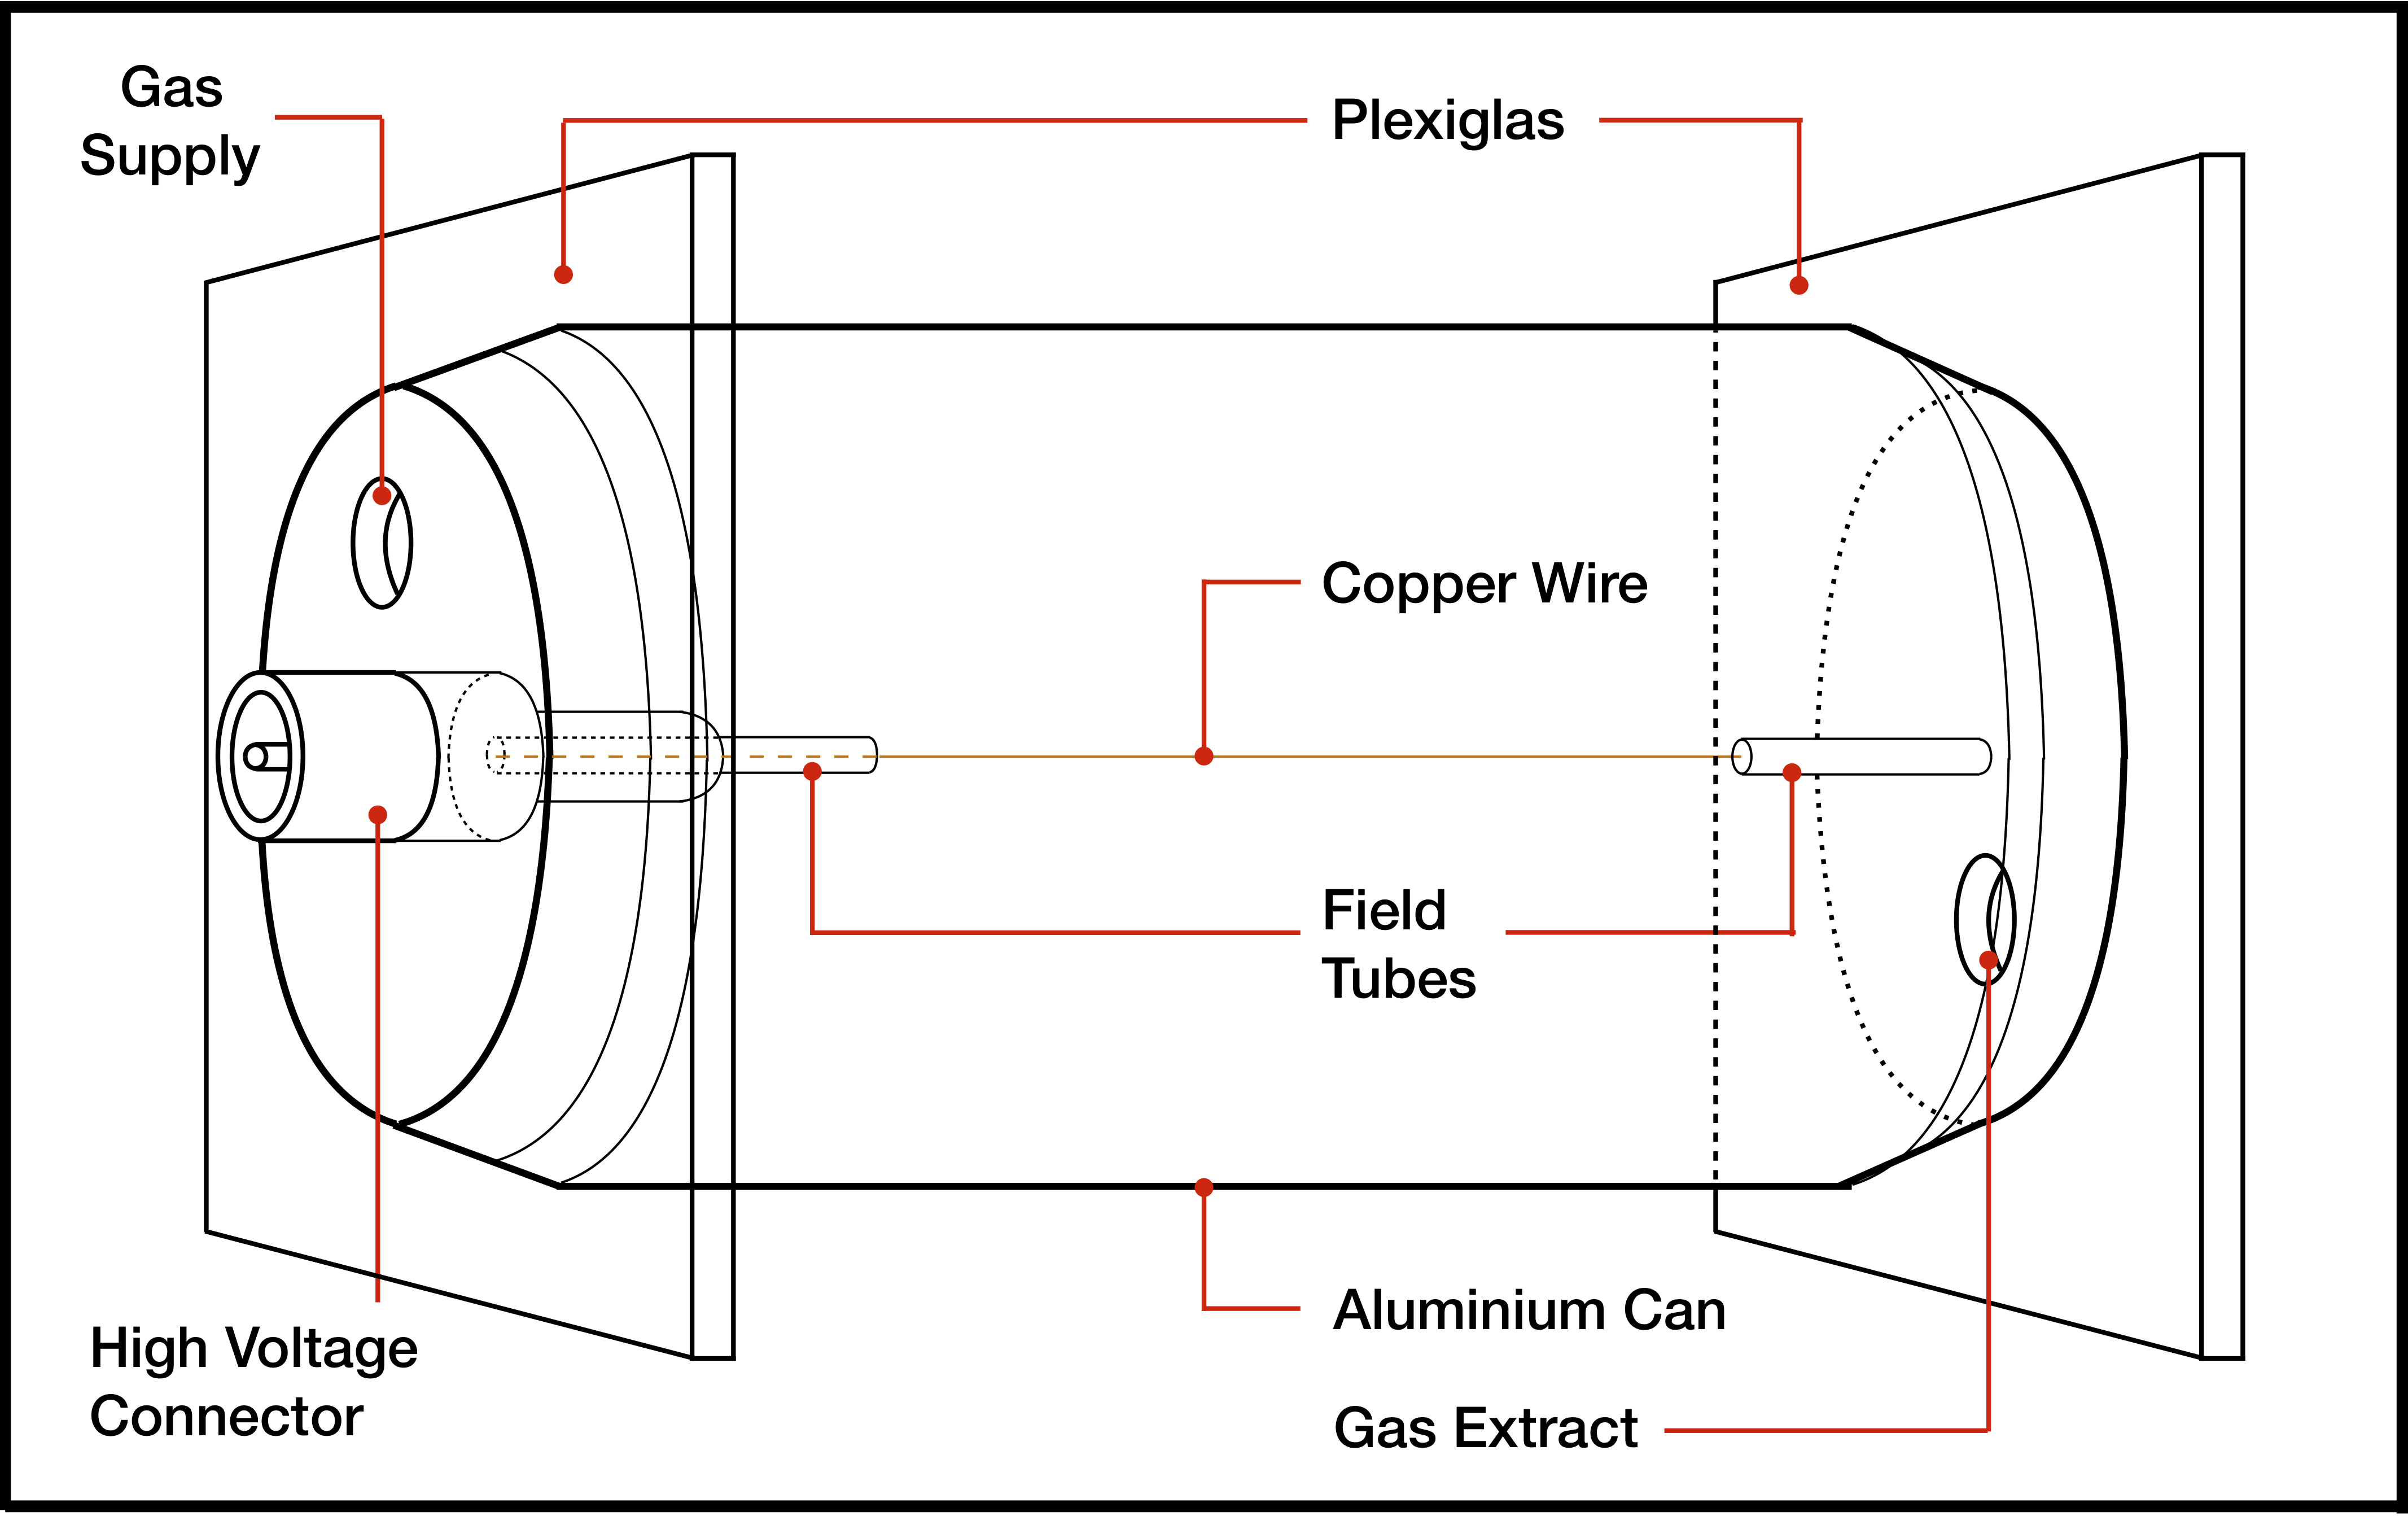
\includegraphics[width=\textwidth]{detectorSchematic.png}
  \caption{Schematic of the detector.}
  \label{fig:schematic}
\end{figure}

\section{Detector Assembly}

For the cathode, an aluminium beverage can was used. The ends were removed using a hole saw drill bit, and filed down with a rat-tail file to ensure there were no sharp points from which sparking could occur. The non-conducting oxide layer on the interior of the can was removed with a stiff sponge attached to a battery powered drill. On the can's exterior, a strip of paint was sanded away with abrasion paper so that an electrical contact to ground could be established. Connectivity was tested with a digital multi-meter to check that the insulating layer had been completely removed. If it was not, the shape of the electric field inside of the detector would not have followed the cylindrical geometry used in the Diethorn formula (Equation \ref{eqn:Diethorn}).

The can's length and diameter were found to be inconsistent when measured at corresponding points around the can. Three measurements were made to give an average and standard error, which exceeded the instrumental uncertainty in both cases. The length and diameter were found to be (111.00$\pm$0.09)mm and (52.8$\pm$0.1)mm respectively. The can wall was directly measured as (0.22$\pm$0.01)mm, however due to the curvature of the can this was not representative of the can wall thickness. By also measuring the diameter of the micrometer spindle and using some simple geometry a rough value for the thickness of the can was found as (0.02$\pm$0.05)mm, however the uncertainty is greater than the value itself and so cannot be trusted.

The ends of the can were covered by Plexiglas endplates, with grooves cut for the can to slot into. Holes were drilled in the endplates: a 9.4mm drill bit was used for the HV connector, 1.0mm for the field tubes and 5.6mm for gas pipes.

A single copper thread was taken from an ordinary braided electrical cable to use as the anode, this had a diameter of approximately (50$\pm$10)\textmu m. Both pieces of field tube were cut from the same length of brass tube with a manufacturer's diameter of 1mm. They were also filed at both ends to prevent sparking. After they had been filed, their lengths were measured as (26.87$\pm$0.02)mm and (13.75$\pm$0.02)mm. A commercial high voltage connector was used to connect the detector to the preamplifier.

Once all the components were prepared and ready for assembly, they were cleaned in isopropanol in an ultrasonic bath for two minutes. This is to remove any dust, grease or flakes of metal which may have accumulated on the components during their preparation. From this point onwards, gloves were worn to keep the components clean.

\begin{figure}[h]
  \centering
  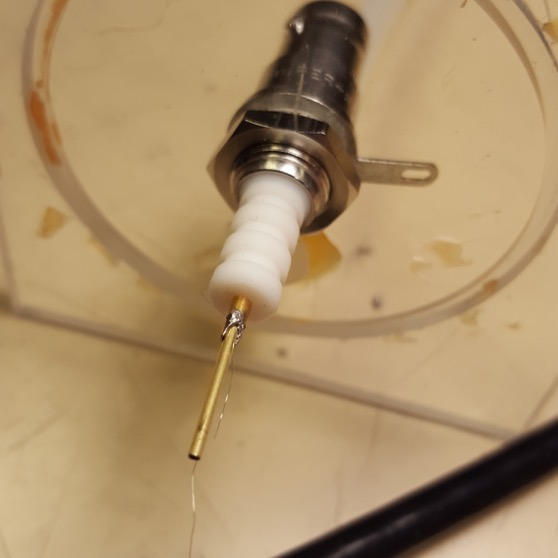
\includegraphics[width=7cm]{HVconnector.jpg}
  \caption{Photograph showing the connection between the anode, field tube, high voltage connector and endplate.}
  \label{fig:HVC}
\end{figure}

The anode was threaded through the shorter field tube until a short length was poking out of the other side. The field tube was then inserted into the high voltage connector with the short length of anode hanging loose outside of the connector. The components were soldered together where the field tube and anode emerged from the high voltage connector securing both in place. The high voltage connector was in turn connected to the endplate using a bolt supplied with the connector (Figure \ref{fig:HVC}).

To glue the components together Araldite glue was used as it also forms an airtight seal around the joints, preventing gas leaks. The longer field tube was glued in the endplate with the 1mm hole, and the anode was threaded through the shielding so that it could be soldered on the other side. Both endplates were taped onto the detector to hold them in place while the anode was pulled taut and soldered -- in case it snapped and the detector needed to be reopened. Once the anode was soldered it was checked to ensure it was taut which is important for ensuring a uniform electric field inside the detector. The endplates were then glued to the can and the gas supply tubes were glued into the endplates. Glue was also applied around the high voltage connector and the free end of the anode to seal the detector.

To reduce noise; insulating Kapton tape was stuck over the free end of the detector. Copper tape was also stuck from the high voltage connector to the conducting strip on the outside of the aluminium can. Finally aluminium shielding was folded around the endplates and grounded by a cable from the high voltage connector (Figure \ref{fig:setup}).

\section{Measurements}

\begin{figure}[h]
  \centering
  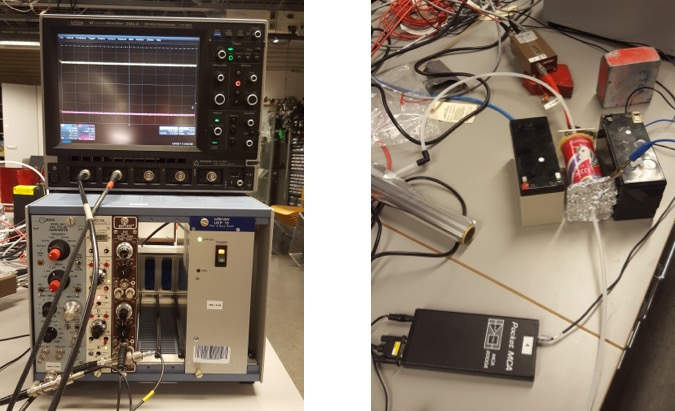
\includegraphics[width=\linewidth]{apparatus.jpg}
  \caption{Photographs of the apparatus used to perform the experiment. Seen in the picture is the Wiener UEP 15 (Power Supply), ComTec MHQ206L (High Voltage Supply), ORTEC 855 Dual Amplifier (Spectroscopic Amplifier), BNC Model BH-1 (Pulse Generator), LeCroy Wavesurfer 24Xs-A (Oscilloscope), ORTEC 142A (Preamplifier) and Amptek MCA8000A (Multichannel Analyser).}
  \label{fig:setup}
\end{figure}

The detector needs to be flushed with P-10 gas before any measurements can be taken, so the seal of the detector was checked first using a gas flow meter. The gas flow supplied to the detector was measured as (10.3$\pm$0.2)ml/min and the gas flow out of the detector was found to be (9.9$\pm$0.2)ml/min which means the detector was sufficiently gas tight. The gas flow was then turned up to reduce the amount of time taken to flush the detector and left for several hours. Once the detector had been satisfactorily flushed, the gas flow was reduced back down to a flow rate of (18.4$\pm$0.2)ml/min.

The detector was connected to the preamplifier via the high voltage connector, which was in turn connected to the high voltage supply and pulse generator. The multichannel analyser was set to measure over the voltage range 10V sorting into 512 bins. Higher resolution is unnecessary since the detector resolution is the limiting factor. The pulse generator, high voltage supply and spectroscopic amplifier (spec amp) were powered by the Wiener power supply to regulate the current and voltage supply to the instruments.

An aluminium collimator was used for taking any measurements using the \textsuperscript{55}Fe source. For the \textsuperscript{241}Am source a lead collimator was used to further reduce the number of gamma rays entering the detetcor per unit time. This is because \textsuperscript{241}Am is a very high activity source and the response time of the detector is too slow to record each gamma ray as an individual event. When using the \textsuperscript{241}Am source a lead shield was also positioned around the detector to minimise exposure to those in the lab.

\subsection{Electron Calibration}

\begin{figure}[h]
  \centering
  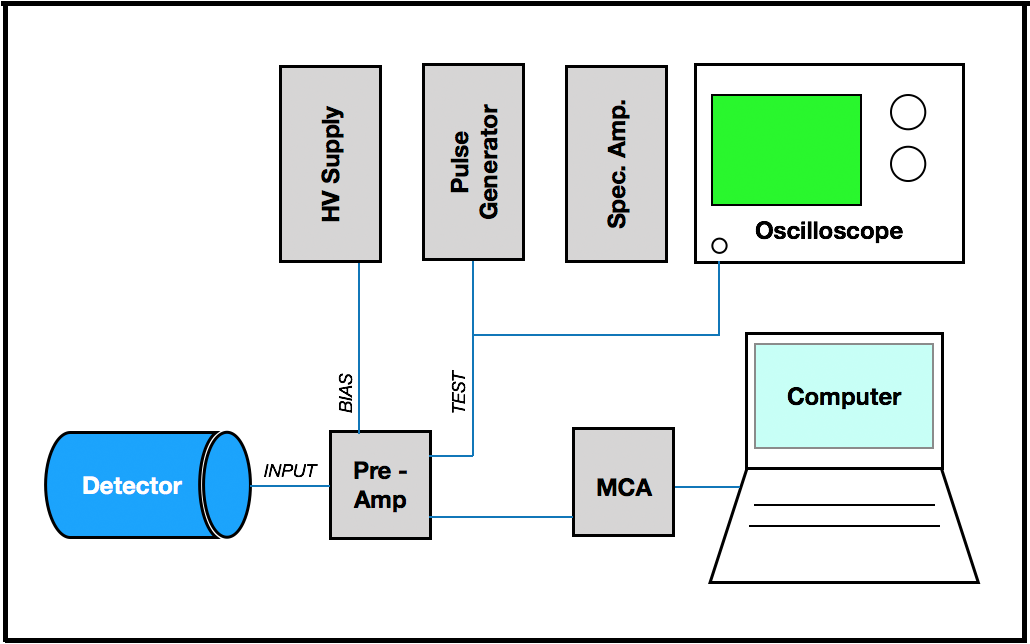
\includegraphics[width=\linewidth]{calibrationSchematic.png}
  \caption{Diagram showing the experimental setup for performing the electron calibration.}
  \label{fig:calibrationSetup}
\end{figure}

To characterise the detector, one must know what MCA channel number corresponds to what detected charge. The pulse generator output was split using a \textquotesingle T\textquotesingle \space connector and connected to the oscilloscope and preamplifier as shown in Figure \ref{fig:calibrationSetup}. The output of the preamplifier was fed straight to the MCA and the high voltage supply was left off. The pulse generator sent pulses to the preamplifier with a rise time of 50ns and a fall time of 50\textmu s to mimic the pulse shape of ionisation events in the detector. The average voltage of the pulses and their standard deviation were measured on the oscilloscope using its built in measurement function. The MCA measured the signal for 10 seconds, sorting the pulses into 512 bins to be displayed on the spectrum software. These measurements were repeated at 10mV intervals from 10mV until 150mV where the pulse exceeded the MCA's 10V limit. This resulted in a series of sharp peaks ranging across the MCA channels (Figure \ref{fig:electronCalibrationData}). The centre, its uncertainty and the full width at half maximum (FWHM) of each peak was then fitted in the software using the built in fitting tool (Table \ref{tbl:electronCalibrationData}).

The preamplifier had a capacitance of 1pF which made it possible to calculate the collected charge from the measured voltage, which in turn enabled the number of collected electrons to be calculated:
\begin{equation}
    C = \frac{Q}{V}
    \label{eqn:C=Q/V}
\end{equation}
\begin{equation}
    n_e = \frac{Q}{e}
    \label{eqn:n_e}
\end{equation}

The errors in the input pulse voltage arose from both statistical error and instrumental error. The statistical error is a result of the spread of values as measured by the oscilloscope, and the instrumental error is specified by the manufacturer as $\pm$1\% of the full scale. Since the full scale was not recorded for each measurement, it will be estimated as $\pm$3\% of the measured pulse voltage because the signal never spanned less than 1/3 of the total scale. These errors were added by quadrature.

Error in the channel also arose due to non-linearities and temperature instability in the preamplifer and MCA, resulting in an error of $\pm$0.185\%. This is insignificant compared to the error from the fit, but was included in calculations for completeness. It was added to the error given by the specutrum software's fitting tool by quadrature.

This data was then plotted and fitted using Python's ODR package, which takes x and y errors into account, to two linear models: one with a constant term and one without. One would expect there to be no constant term since channel number should read zero when the pulse voltage is zero, and the uncertainty for the constant term when fitted is very large compared to its actual value, which supports this (Figure \ref{fig:calibration}). For this reason the model with no constant term was used to produce the calibration equation.

\subsection{Voltage Scan} \label{sec:mthd:voltageRun}

\begin{figure}[h]
  \centering
  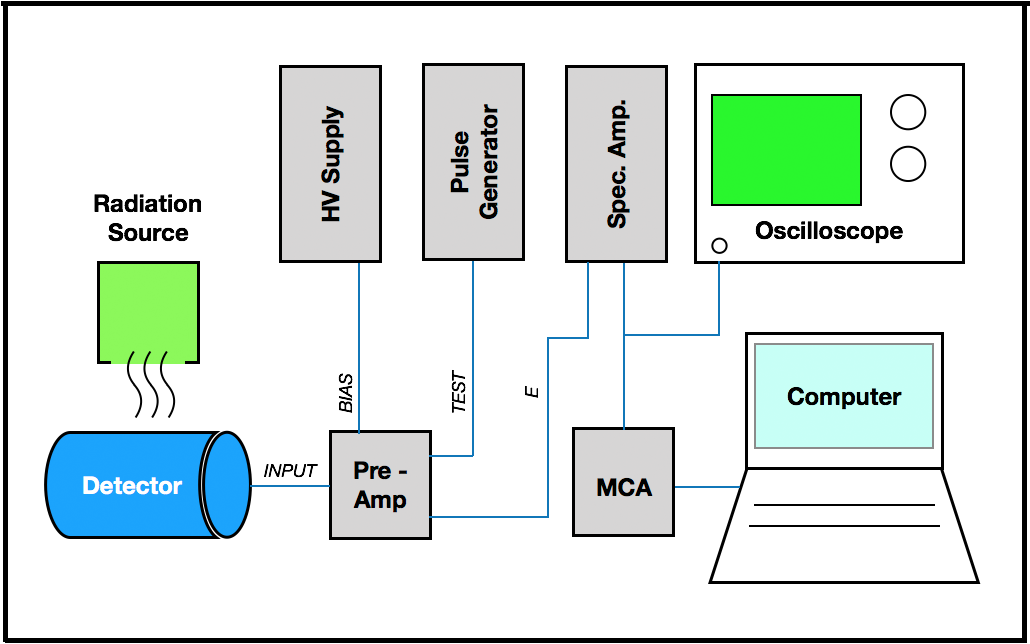
\includegraphics[width=\linewidth]{scanSchematic.png}
  \caption{Diagram showing the experimental setup for performing the voltage scan.}
  \label{fig:scanSetup}
\end{figure}

To test the proportionality of the detector, the collected charge was measured as a function of applied voltage. To perform these measurements the pulse generator was turned off and the high voltage supply was turned on. The signal from the preamplifier was now sent to a spec amp which was set to its maximum gain, and was then split between the oscilloscope and the MCA using a \textquotesingle T\textquotesingle connector.
The high voltage supply was then gradually increased until a signal was observed on the oscilloscope. For \textsuperscript{55}Fe this was observed at 1520V.

The spectrum was then measured for 60 seconds at 50V increments on the high voltage power supply. The spectrum software was used to fit to \textsuperscript{55}Fe's main photopeak, giving the peak centre, its uncertainty and the FWHM. When the spectrum filled the MCA's channels; without changing the voltage, the coarse gain was reduced by one increment so that systematic errors arising from nonlinearities in the spec amp coarse gain could be estimated. This was repeated until spectrum filled the MCA channels at the lowest spec amp gain.

The \textsuperscript{55}Fe sample and aluminium collimater were then swapped for the \textsuperscript{241}Am and lead collimator, and the voltage was reduced until the spectrum fitted in the MCA's channel range. Working in the opposite direction to before, the spectrum was then measured for 180 seconds before reducing the high voltage supply in 50V increments, taking the same measurements as before. When the spectrum filled only the lower channels of the MCA, the coarse gain was increased and the process repeated until the coarse gain was at its maximum.

Using the channel number and the conversion equation, the number of detected electrons from the \textsuperscript{55}Fe and \textsuperscript{241}Am photopeaks can be plotted against the high voltage supply.

Error in the high voltage scan came from fluctuations in the readout during the measurement of $\pm$1V. There was also instrumental error specified by the manufacturer of $\pm$(0.05\%V + 0.02\%V\textsubscript{max} + 1 digit per year), where V is the measured voltage in kV, V\textsubscript{max} is the maximum voltage in kV (6kV for this instrument) and 1V was added since the high voltage supply was one year old. These two uncertainties were added by quadrature.

Error in the number of detected electrons came from the statistical error from the spectrum software fit and instrumental error from the preamplifier and MCA as before, but this time the spec amp gain is changed and therefore contributes to the error as well. The spec amp has errors stated by the manufacturer attributed to non-linearities (which are not important as fine gain was not changed) and temperature instability. As well as these, it can be seen that there are discontinuities in the number of detected electrons when the coarse gain is changed. This error was taken into account by summing the absolute value of the discontinuities in channel number over the whole range of measurements. Choosing to use a constant error was motivated by the fact that the size of the error did not increase in size at higher gains and there is no reason to believe the spec amp is more accurate at a lower gain. These two errors were added by quadrature.

\subsection{Multiplication Factor}

To calculate the multiplication factor, the ratio of electrons produced in the detector to the number of electrons produced in the original ionisation event must be determined. The number of electrons produced in the detector was calculated when performing the voltage run so this number simply needs to be divided by the number of original ions, given by Equation \ref{eqn: n_0}.

A book value was used for W \cite{Wolff_W_dV_K} which has no uncertainty quoted so the only uncertainty in the multiplication factor calculation is carried through from the uncertainty in the number of detected electrons:
\begin{equation}
    \Delta M = \frac{\Delta n_{e}}{n_{i}}
\end{equation}

The theoretical Diethorn equation (Equation \ref{eqn:Diethorn}) was plotted on the same graph, using book values for $\Delta$V and K \cite{Wolff_W_dV_K}. The uncertainty limits are given by:
\begin{equation}
    \lambda = \ln{\bigg( \frac{b}{a} \bigg)}
\end{equation}
\begin{equation}
    \Delta \lambda = \sqrt{\bigg(\frac{\Delta a}{a}\bigg)^{2} + \bigg(\frac{\Delta b}{b}\bigg)^{2}}
\end{equation}
\begin{equation}
    \zeta = \ln{\bigg(\frac{V}{paK\lambda}\bigg)}
\end{equation}
\begin{equation}
    \Delta \zeta = \sqrt{\bigg(\frac{\Delta V}{V}\bigg)^{2} + \bigg(\frac{\Delta p}{p}\bigg)^{2} + \bigg(\frac{\Delta a}{a}\bigg)^{2} + \bigg(\frac{\Delta K}{K}\bigg)^{2} + \bigg(\frac{\Delta \lambda}{\lambda}\bigg)^{2}}
\end{equation}
\begin{equation}
    \Delta M = M \cdot \sqrt{\bigg(\frac{\Delta V}{V}\bigg)^{2} + \bigg(\frac{\Delta \lambda}{\lambda}\bigg)^{2} + \bigg(\frac{\Delta (\Delta V)}{(\Delta V)}\bigg)^{2} + \bigg(\frac{\Delta \zeta}{\zeta}\bigg)^{2}}
\end{equation}

\subsection{Energy Resolution}

To calculate the energy resolution of the detector, the ratio of the full width at half maximum (FWHM) to centroid channel is taken. Using the data collected in the voltage run, a graph was plotted of FWHM against centroid channel, both corrected for gain, for \textsuperscript{55}Fe and \textsuperscript{241}Am. This way it was easy to identify whether spec amp gain has an impact on the energy resolution. A straight line with no constant term was fitted to the plots, taking into account centroid channel uncertainty, and the gradient was the energy resolution (Figures \ref{fig:energyResolutionFe}, \ref{fig:energyResolutionAm}).

A separate graph was also plotted to determine whether there is any correlation between energy resolution and applied voltage.

\subsection{Spectra} \label{sec:mthd:spectra}

The spectra of both \textsuperscript{55}Fe and \textsuperscript{241}Am were measured with their respective collimators, an applied voltage of (1777$\pm$5)V and a spec amp gain of 10. The \textsuperscript{55}Fe source was measured for 313 seconds and the \textsuperscript{241}Am source for 374 seconds. The spectra could be normalised by plotting in terms of intensity (counts divided by measurement time).

The \textsuperscript{55}Fe spectrum resembles two Gaussian curves and python's non-linear least squares algorithm was used to fit a model consisting of two Gaussian curves and a constant background. This gave a good fit however as previously discussed (Chapter \ref{sec:intr:radiationSources}), the main photopeak actually consists of two superimposed peaks a new model was fitted consisting of three Gaussian curves and a constant background, proving to be an even better fit.

It was harder to fit peaks to the \textsuperscript{241}Am spectrum which had a far more complex spectrum. The spectrum was taken to WebPlotDigitizer where an estimate of the background was traced from the original spectrum. This was modelled by two exponential functions multiplied by a fermi function:
\begin{equation}
    Background = (a_{1}e^{b_{1}x}+a_{2}e^{b_{2}x})(1+e^{\frac{x-c}{d}})^{-1}
\end{equation}
This was fitted using python's non-linear least squares algorithm and this background curve was subtracted from the original spectrum leaving just the peaks. The necessary parameters for Gaussian curves were estimated for each of the 5 peaks. Finally, a model was built from the background model plus five Gaussian curves. The parameters previously estimated were used as first guess values and the complete model was successfully fitted with improved accuracy for the parameters.

The fitted peaks were labelled from 1-3 for the \textsuperscript{55}Fe spectrum and from 4-8 for the \textsuperscript{241}Am spectrum, in ascending order of 
channel number (Figures \ref{fig:Fe55spec}, \ref{fig:Am241spec}).

\subsection{Energy Calibration}

As a result of fitting gaussian curves to the spectra, the centres all the spectral peaks are now known. Some of these peaks are very well defined and can be used to determine the relationship between channel number and radiation energy.

Peak 1 is the argon escape peak which has an energy of 3.19keV. Peaks 2 and 3 can be attributed to the relaxation of \textsuperscript{55}Fe's daughter nucleus \textsuperscript{55}Mn with energies of 5.89keV and 6.42keV respectively. Peak 8 produced by a transition in \textsuperscript{241}Am's daughter nucleus \textsuperscript{237}Np which prodcues a gamma ray with an energy of 59.54keV.

By modelling the relationship between peak centre channels against their energies as a straight line, a conversion equation can be determined (Figure \ref{fig:energyCalibration}).

\section{Preamplifier}

\begin{figure}[h]
  \centering
  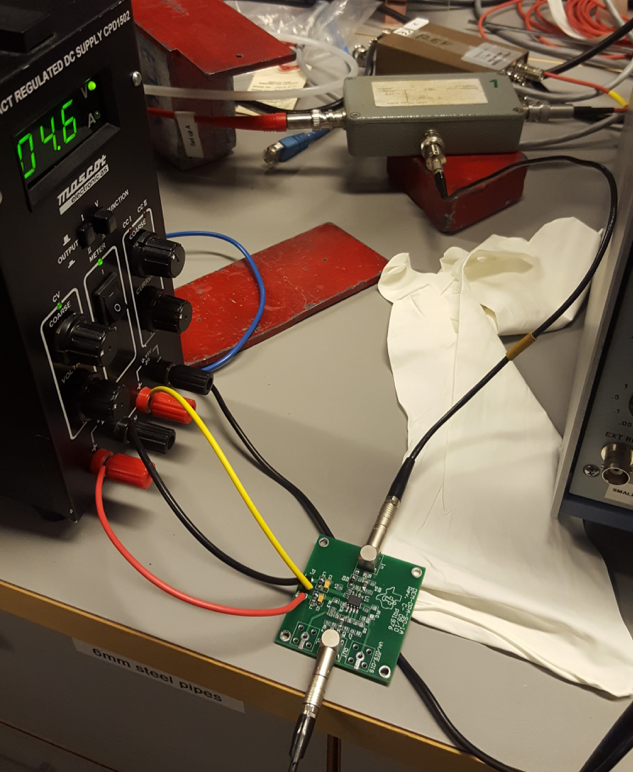
\includegraphics[width=9cm]{preampSpectrumSetup.png}
  \caption{Experimental setup using the kit preamplifier to measure the spectrum of \textsuperscript{55}Fe.}
  \label{fig:preampSpecSetup}
\end{figure}

The preamplifer was assembled from a kit produced by Texas Instruments. The resistors chosen had resistances of 470$\Omega$ and 22$\times10^{6}\Omega$, which gives an expected gain of 46.8.

The gain was checked using the pulse generator and oscilloscope and measuring the ratio of the input pulse voltage from the pulse generator to the output voltage from the preamplifier on the oscilloscope.

The same setup was used as for measuring the spectrum as in Section \ref{sec:mthd:spectra}, only the ORTEC preamplifier is replaced with a decoupler. This is uses capacitance decoupling to output only the signal to the kit preamplifier, as seen in Figure \ref{fig:preampSpecSetup}.

The power supply to the preamplifier was turned up to 4.6V, and the \textsuperscript{55}Fe positioned above the detector on its aluminium collimator. The high voltage supply to the detector was ramped up to 2317V and the coarse gain on the spec amp set to 10. The spectrum was measured for 180 seconds. The dominating source of error in this setup is now the preamplifier and can be estimated using the resistor tolerances.

The spectrum was plotted and fitted using a single gaussian fit about the main photopeak, so that the energy resolution could be compared to the \textsuperscript{55}Fe spectrum taken using the ORTEC preamplifier.
%%%%%%%%%%%%%%%%%%%%%%%%%%%%


%%%%%%%%%%%%%%%%%%%%%%%%%%%%
% RESULTS

\chapter{Results}

\section{Detector}

\subsection{Electron Calibration}

\begin{figure}[H]
  \centering
  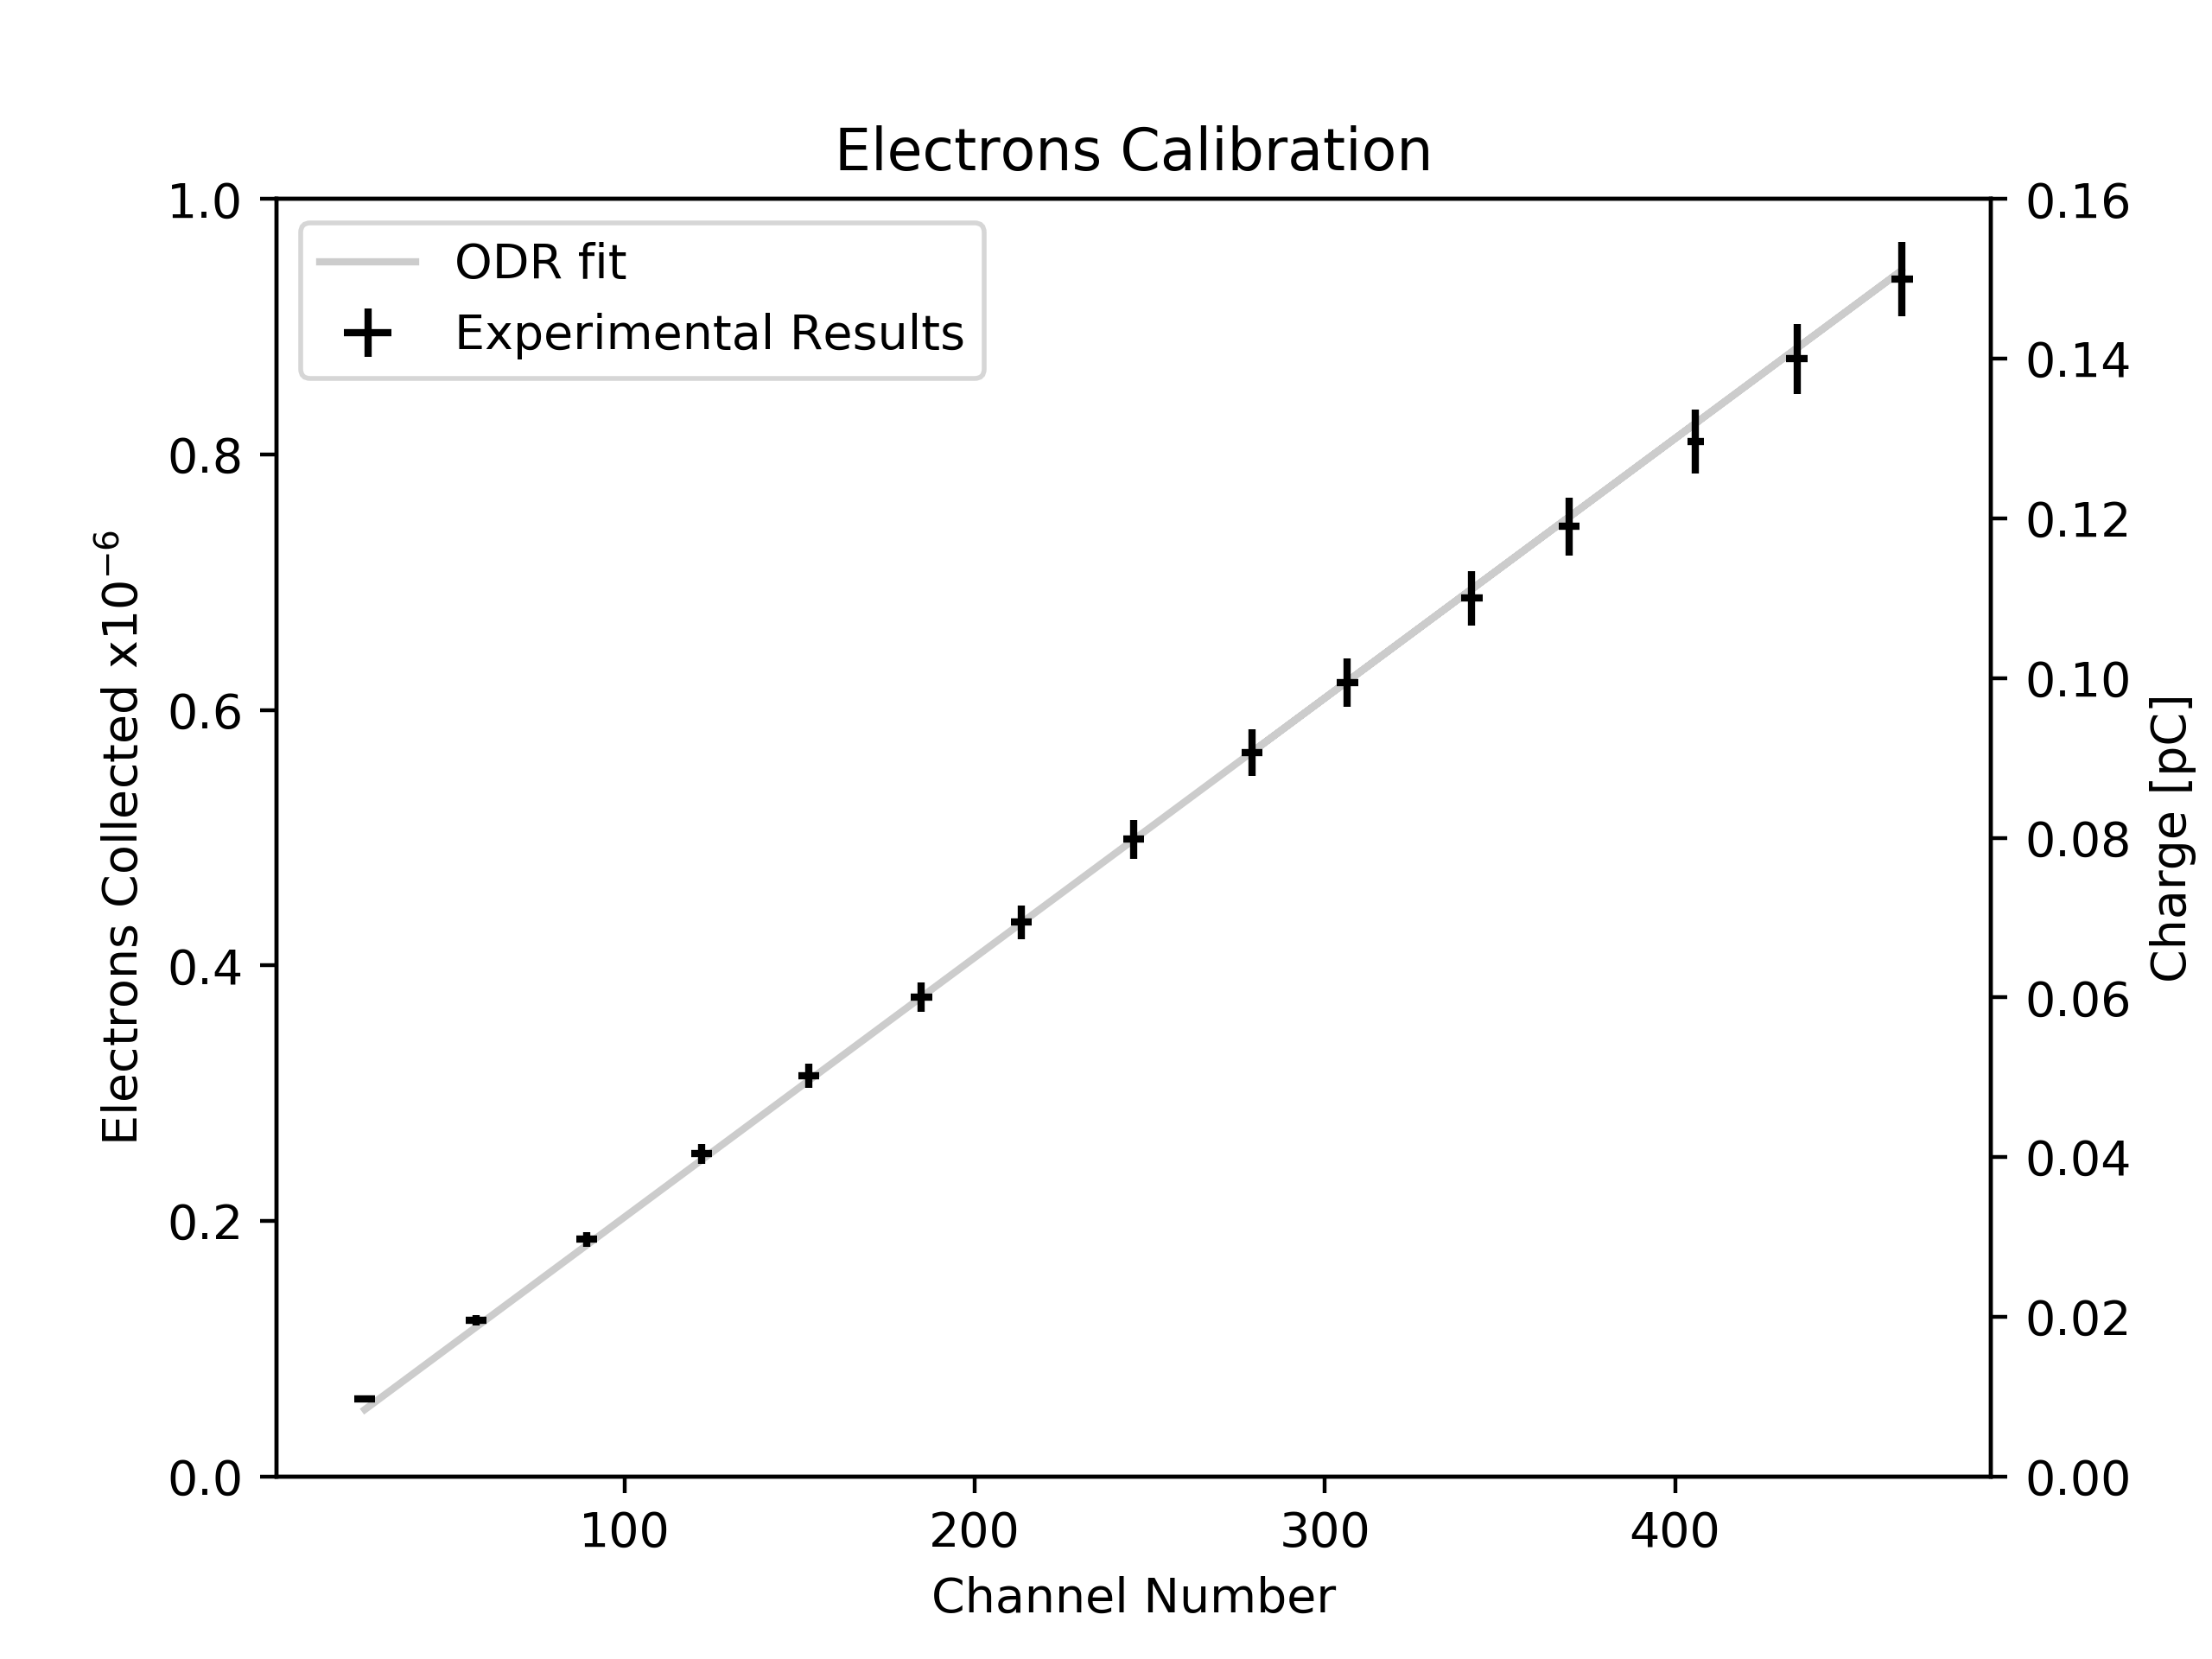
\includegraphics[width=\linewidth]{electronCalibration.png}
  \caption{Graph showing the relationship between MCA channel and the number of collected electrons. The line equation of the best fit line was $n_{e} = (2030\pm20)Ch$. Fitting a model with a constant term gave a line equation of $n_{e} = (1990\pm30)Ch + (8000\pm5000)$ which has a higher uncertainty.}
  \label{fig:calibration}
\end{figure}

\subsection{Voltage Run}

\begin{figure}[H]
  \centering
  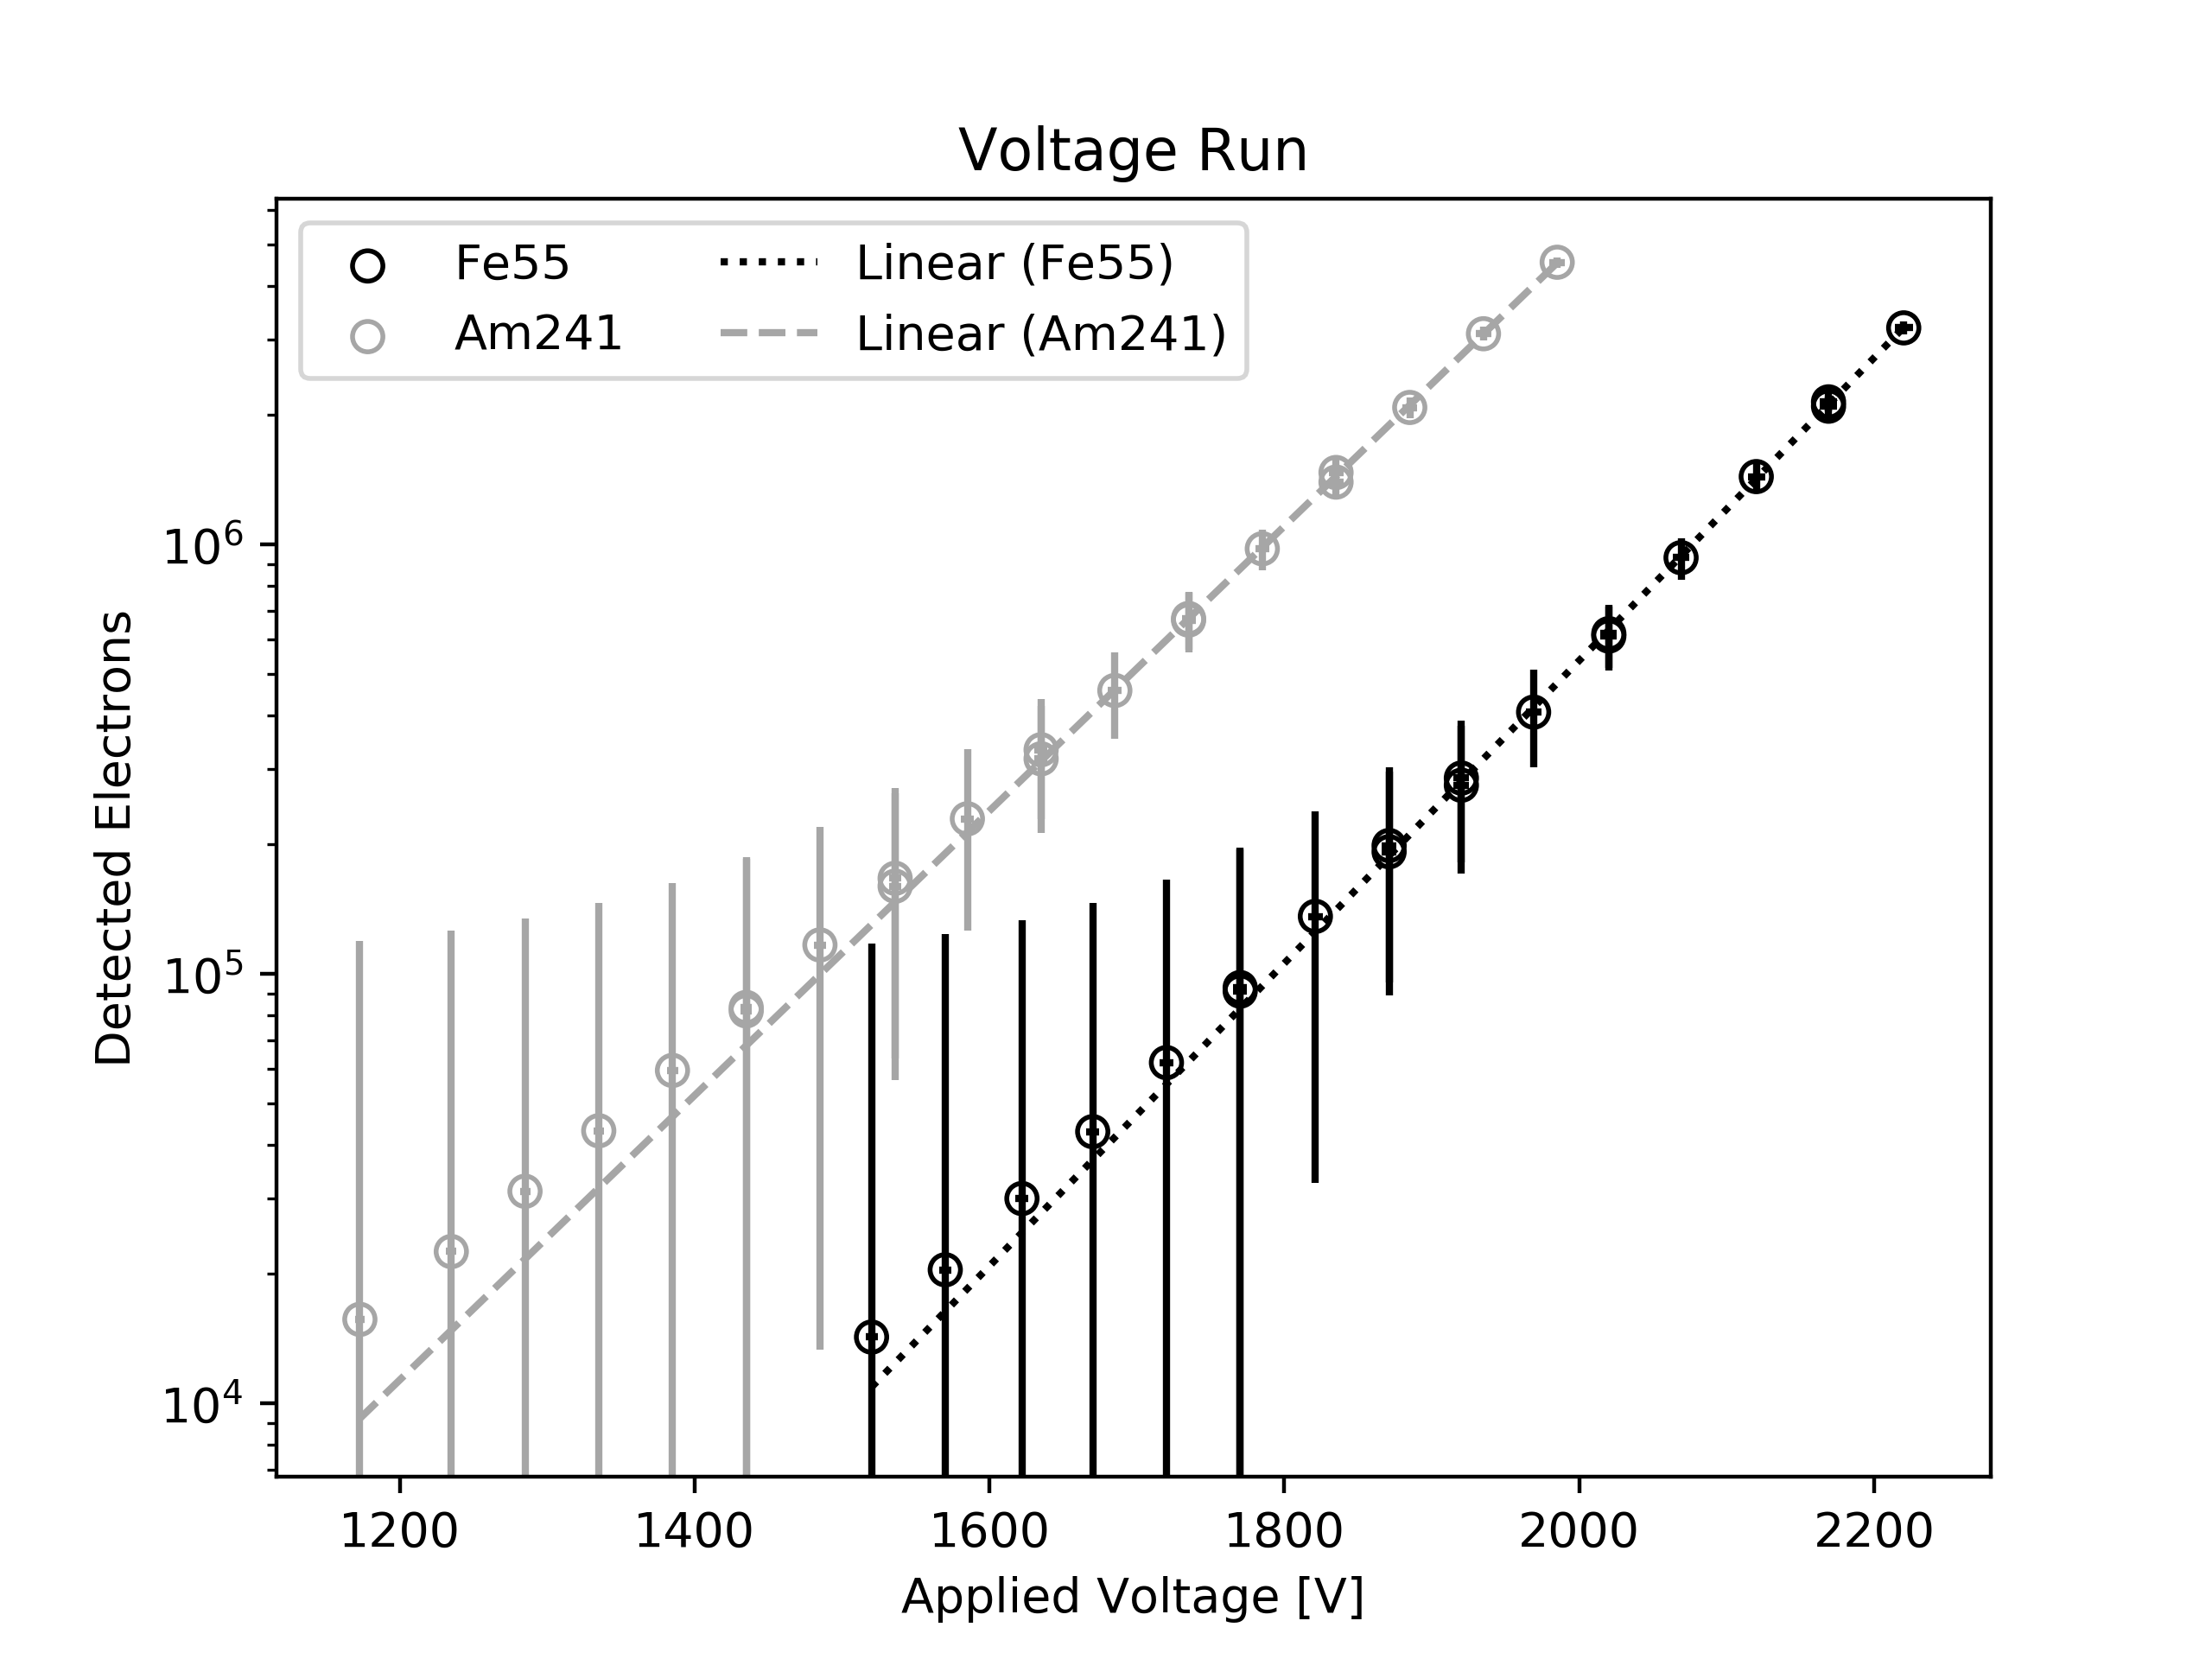
\includegraphics[width=11cm]{voltageRun.png}
  \caption{Results of the voltage run. The distribution for \textsuperscript{55}Fe and \textsuperscript{241}Am can be fitted by exponential functions: $n_{e}(Fe) = (0.05\pm0.04)\cdot\exp{(0.0081\pm0.0004)}$; $n_{e}(Am) = (1.2\pm0.6)\cdot\exp{(0.0076\pm0.0002)}$}
  \label{fig:voltageRun}
\end{figure}

\subsection{Multiplication Factor}

\begin{figure}[H]
  \centering
  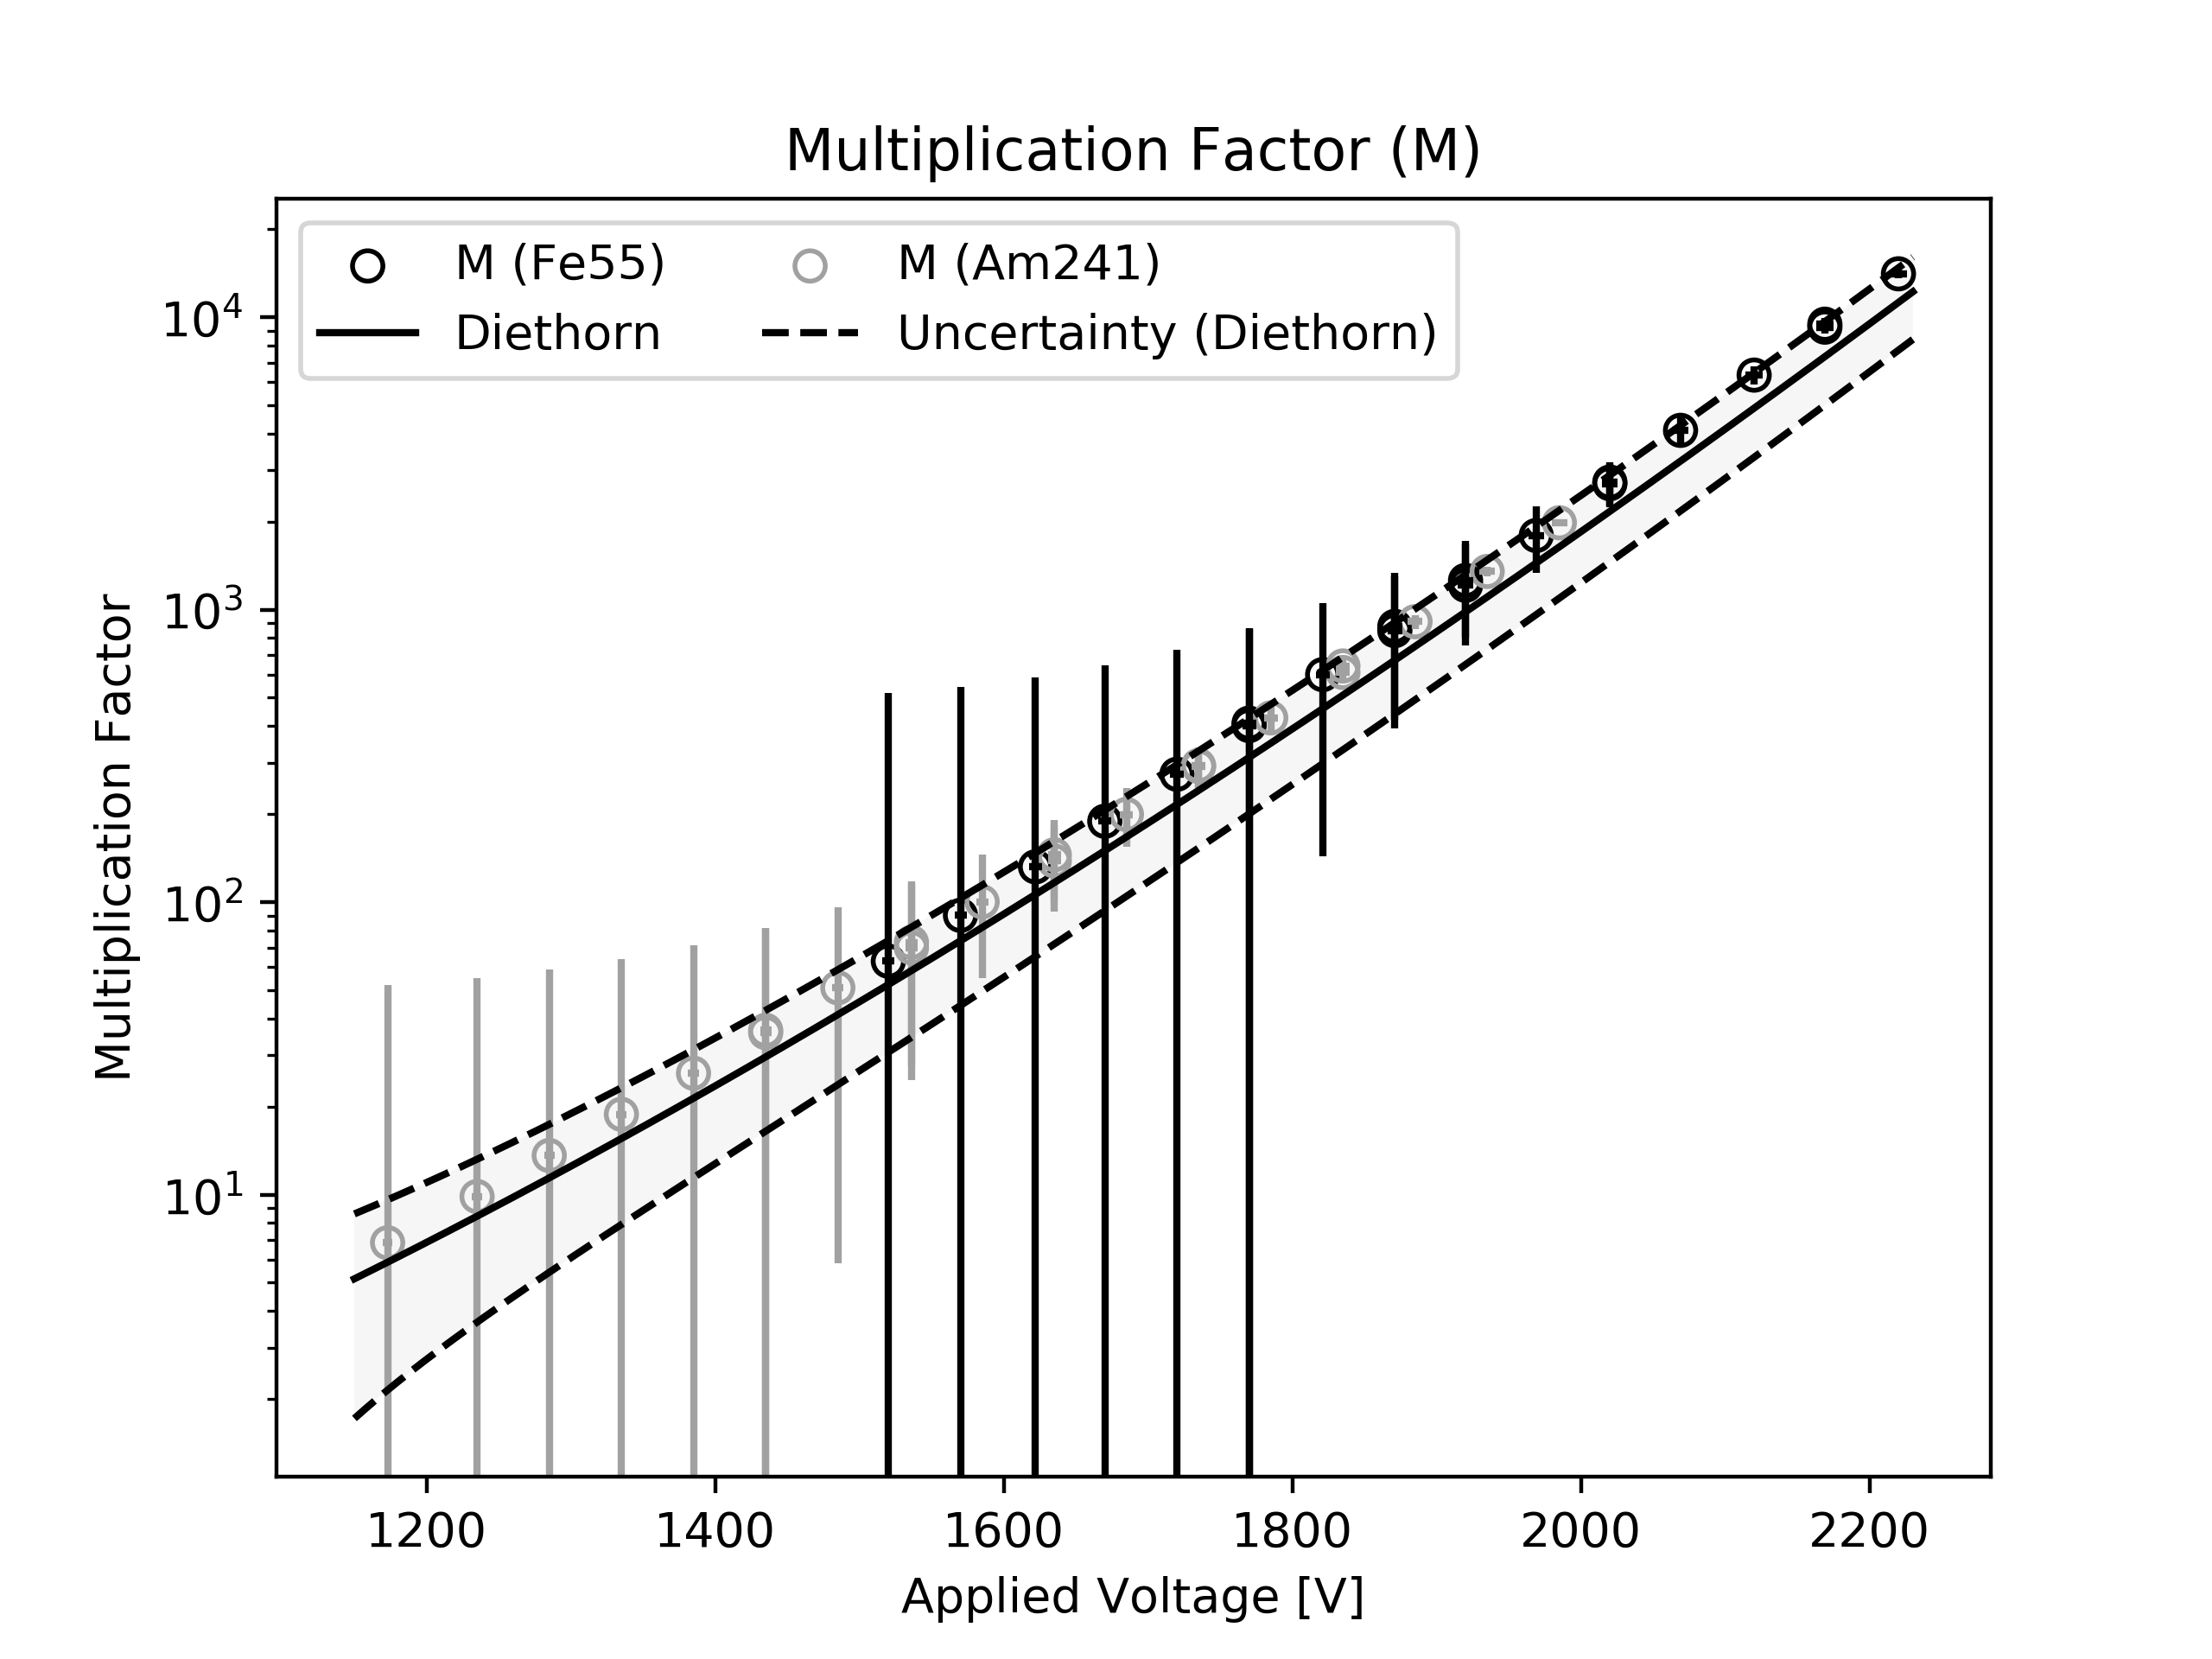
\includegraphics[width=11cm]{mFactor.png}
  \caption{Comparison of measured multiplication factor with the theoretical Diethorn formula.}
  \label{fig:mFactor}
\end{figure}

\subsection{Energy Resolution}

\begin{figure}[H]
  \centering
  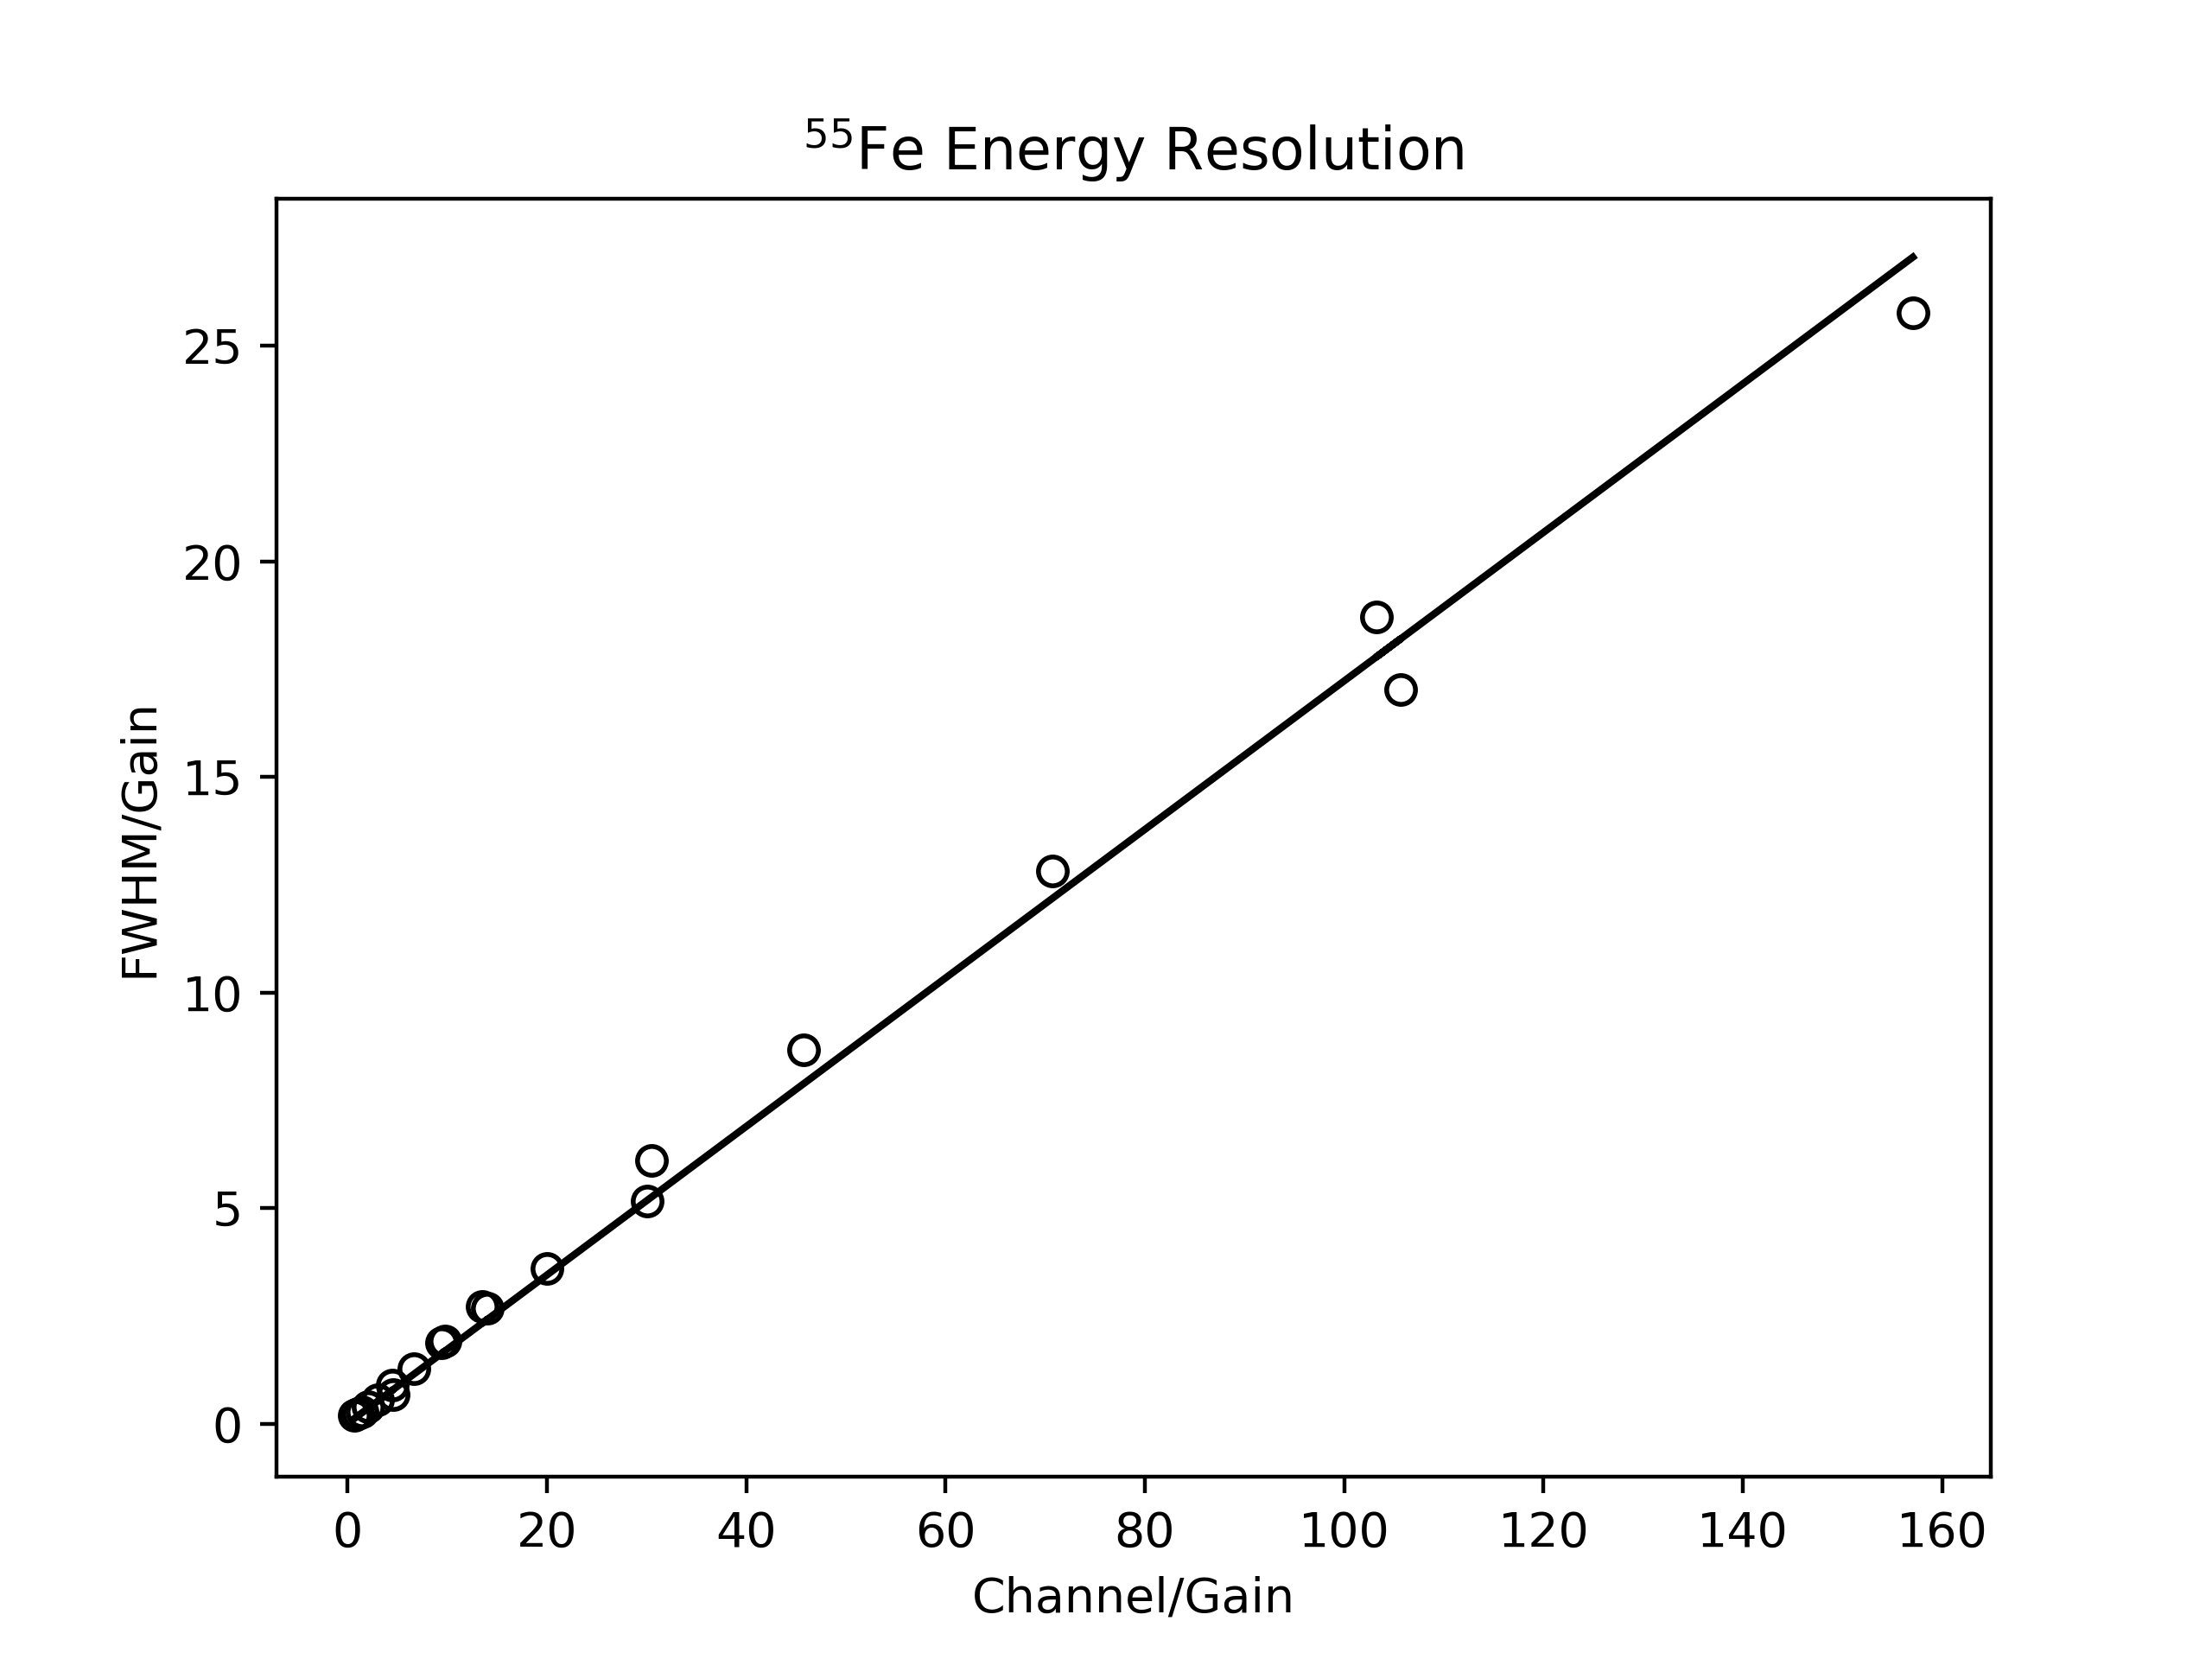
\includegraphics[width=12cm]{energyResolutionFe.png}
  \caption{Graph of gain corrected FWHM against centroid channel for \textsuperscript{55}Fe. The gradient of the trend line is E\textsubscript{res} = (17.2$\pm$0.5)\%.}
  \label{fig:energyResolutionFe}
\end{figure}

\begin{figure}[H]
  \centering
  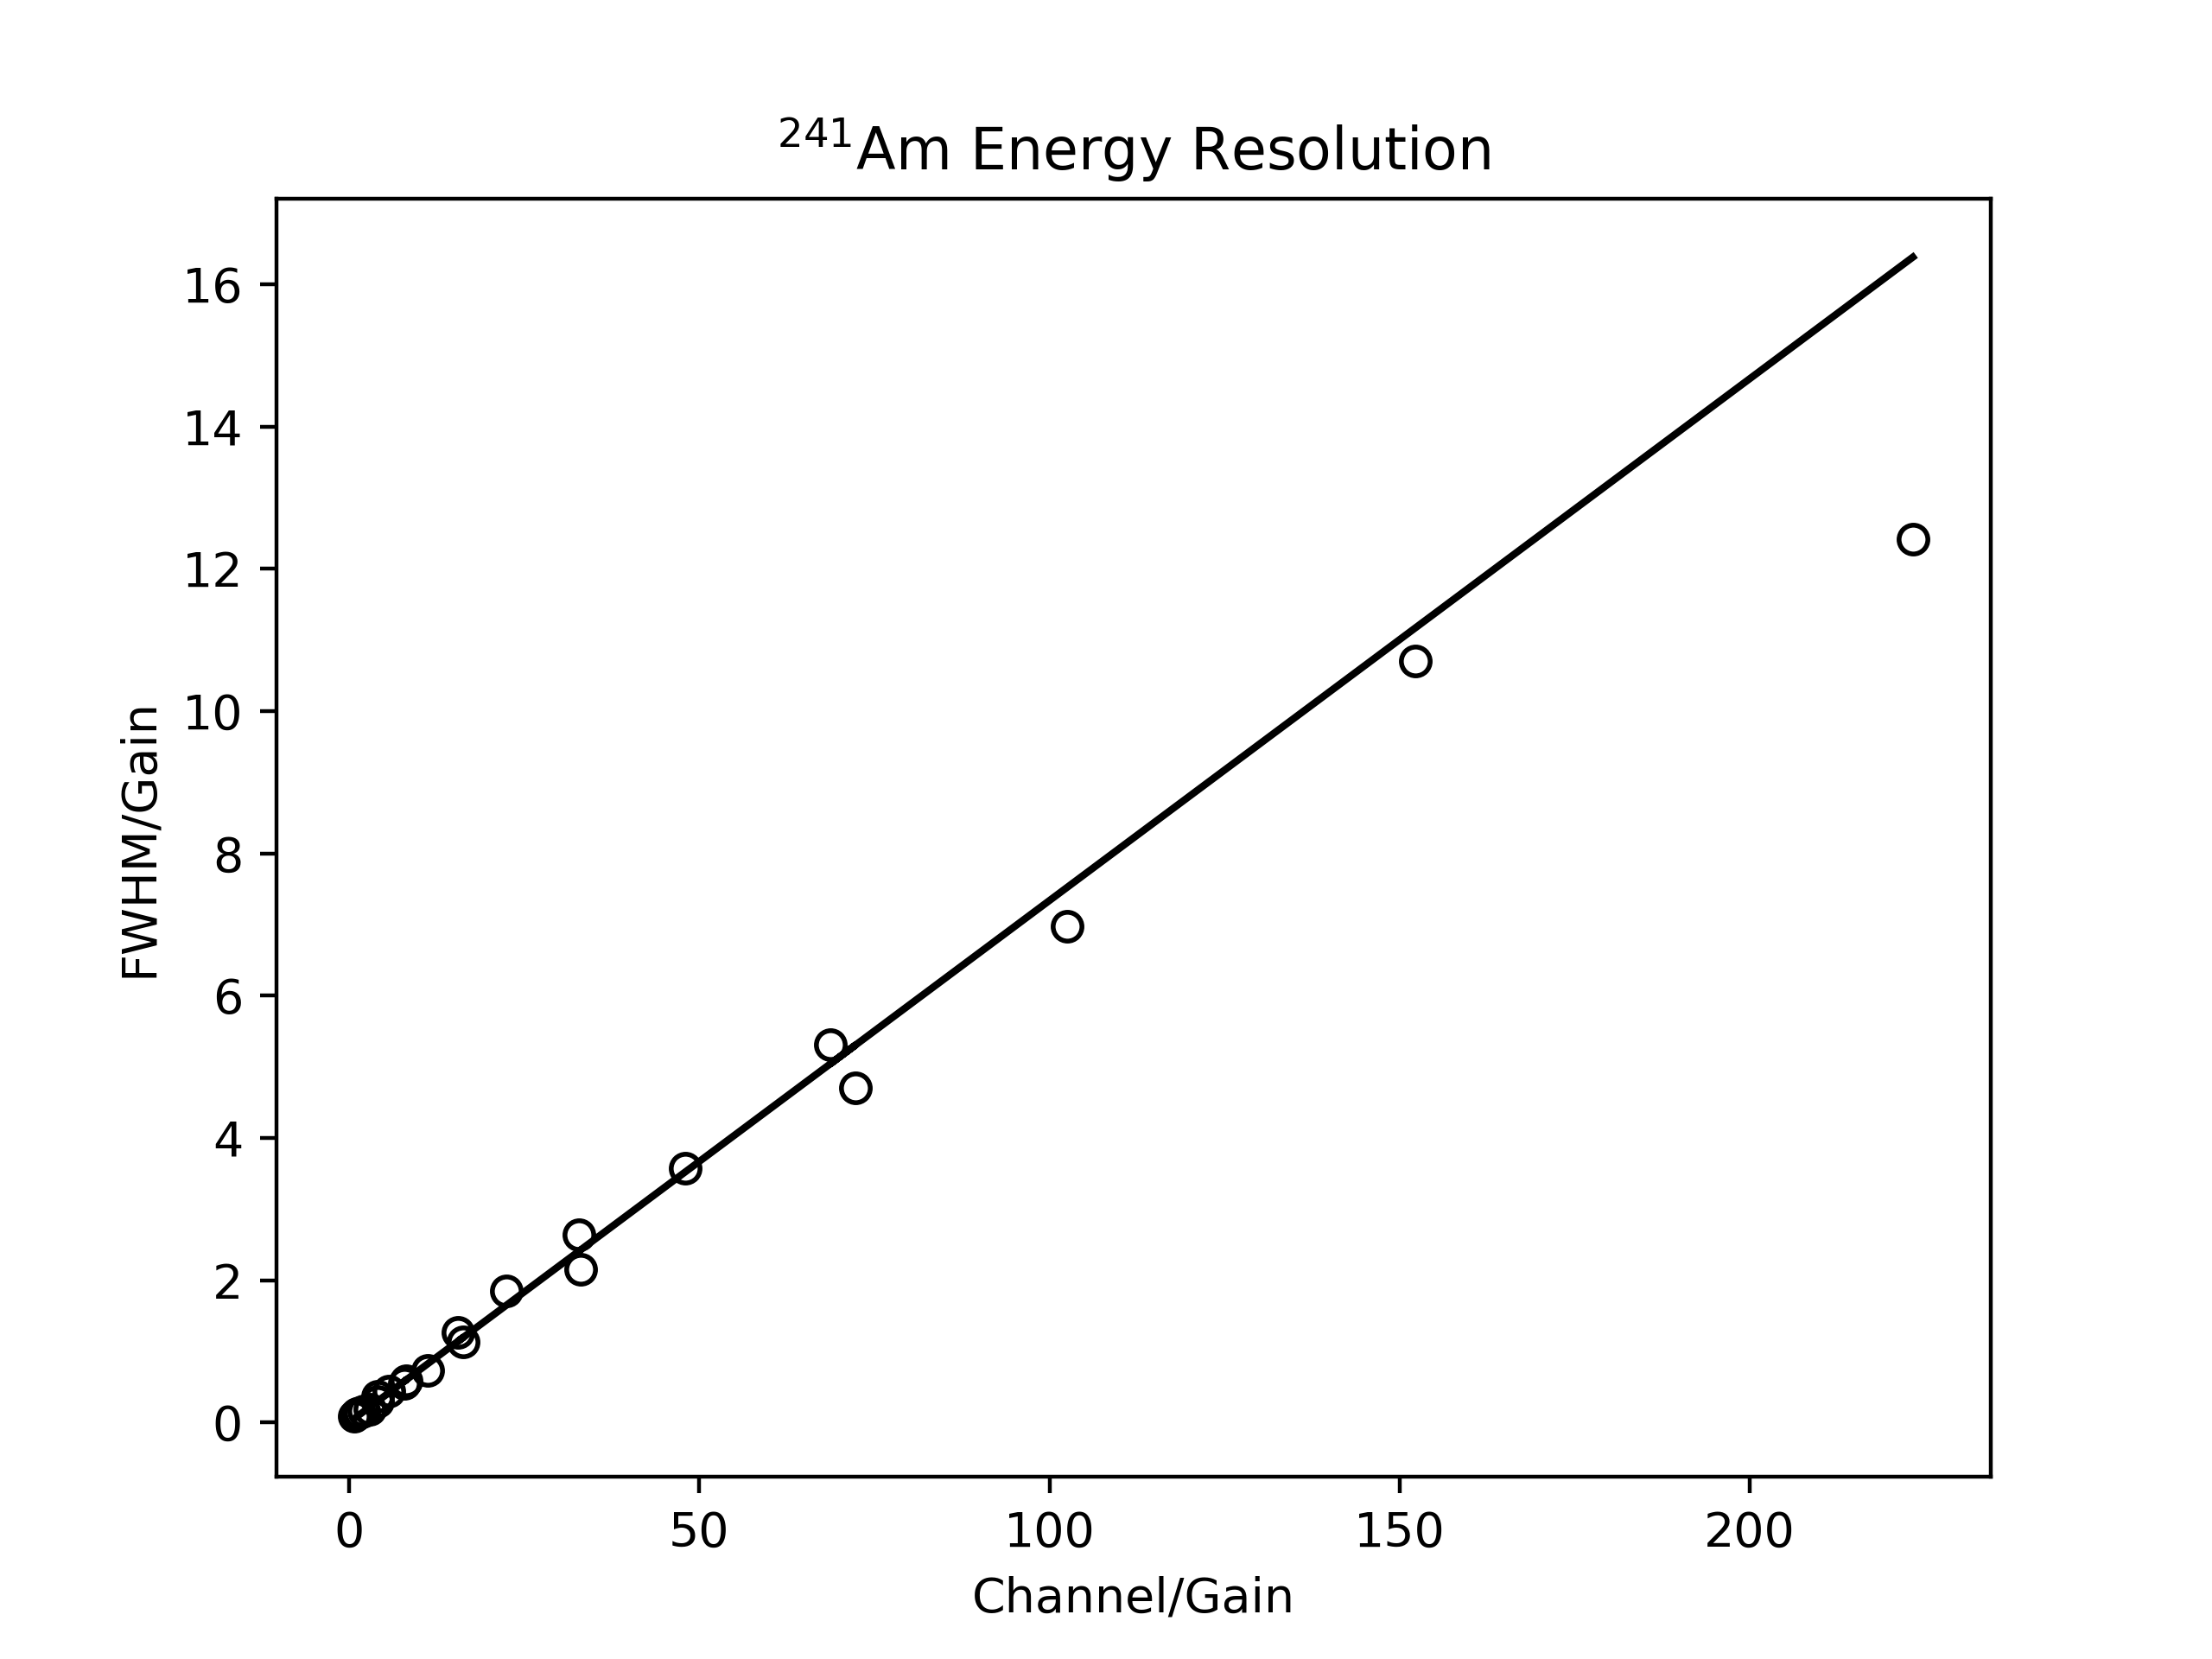
\includegraphics[width=12cm]{energyResolutionAm.png}
  \caption{Graph of gain corrected FWHM against centroid channel for \textsuperscript{241}Am. The gradient of the trend line is E\textsubscript{res} = (7.3$\pm$0.2)\%.}
  \label{fig:energyResolutionAm}
\end{figure}

\begin{figure}[H]
  \centering
  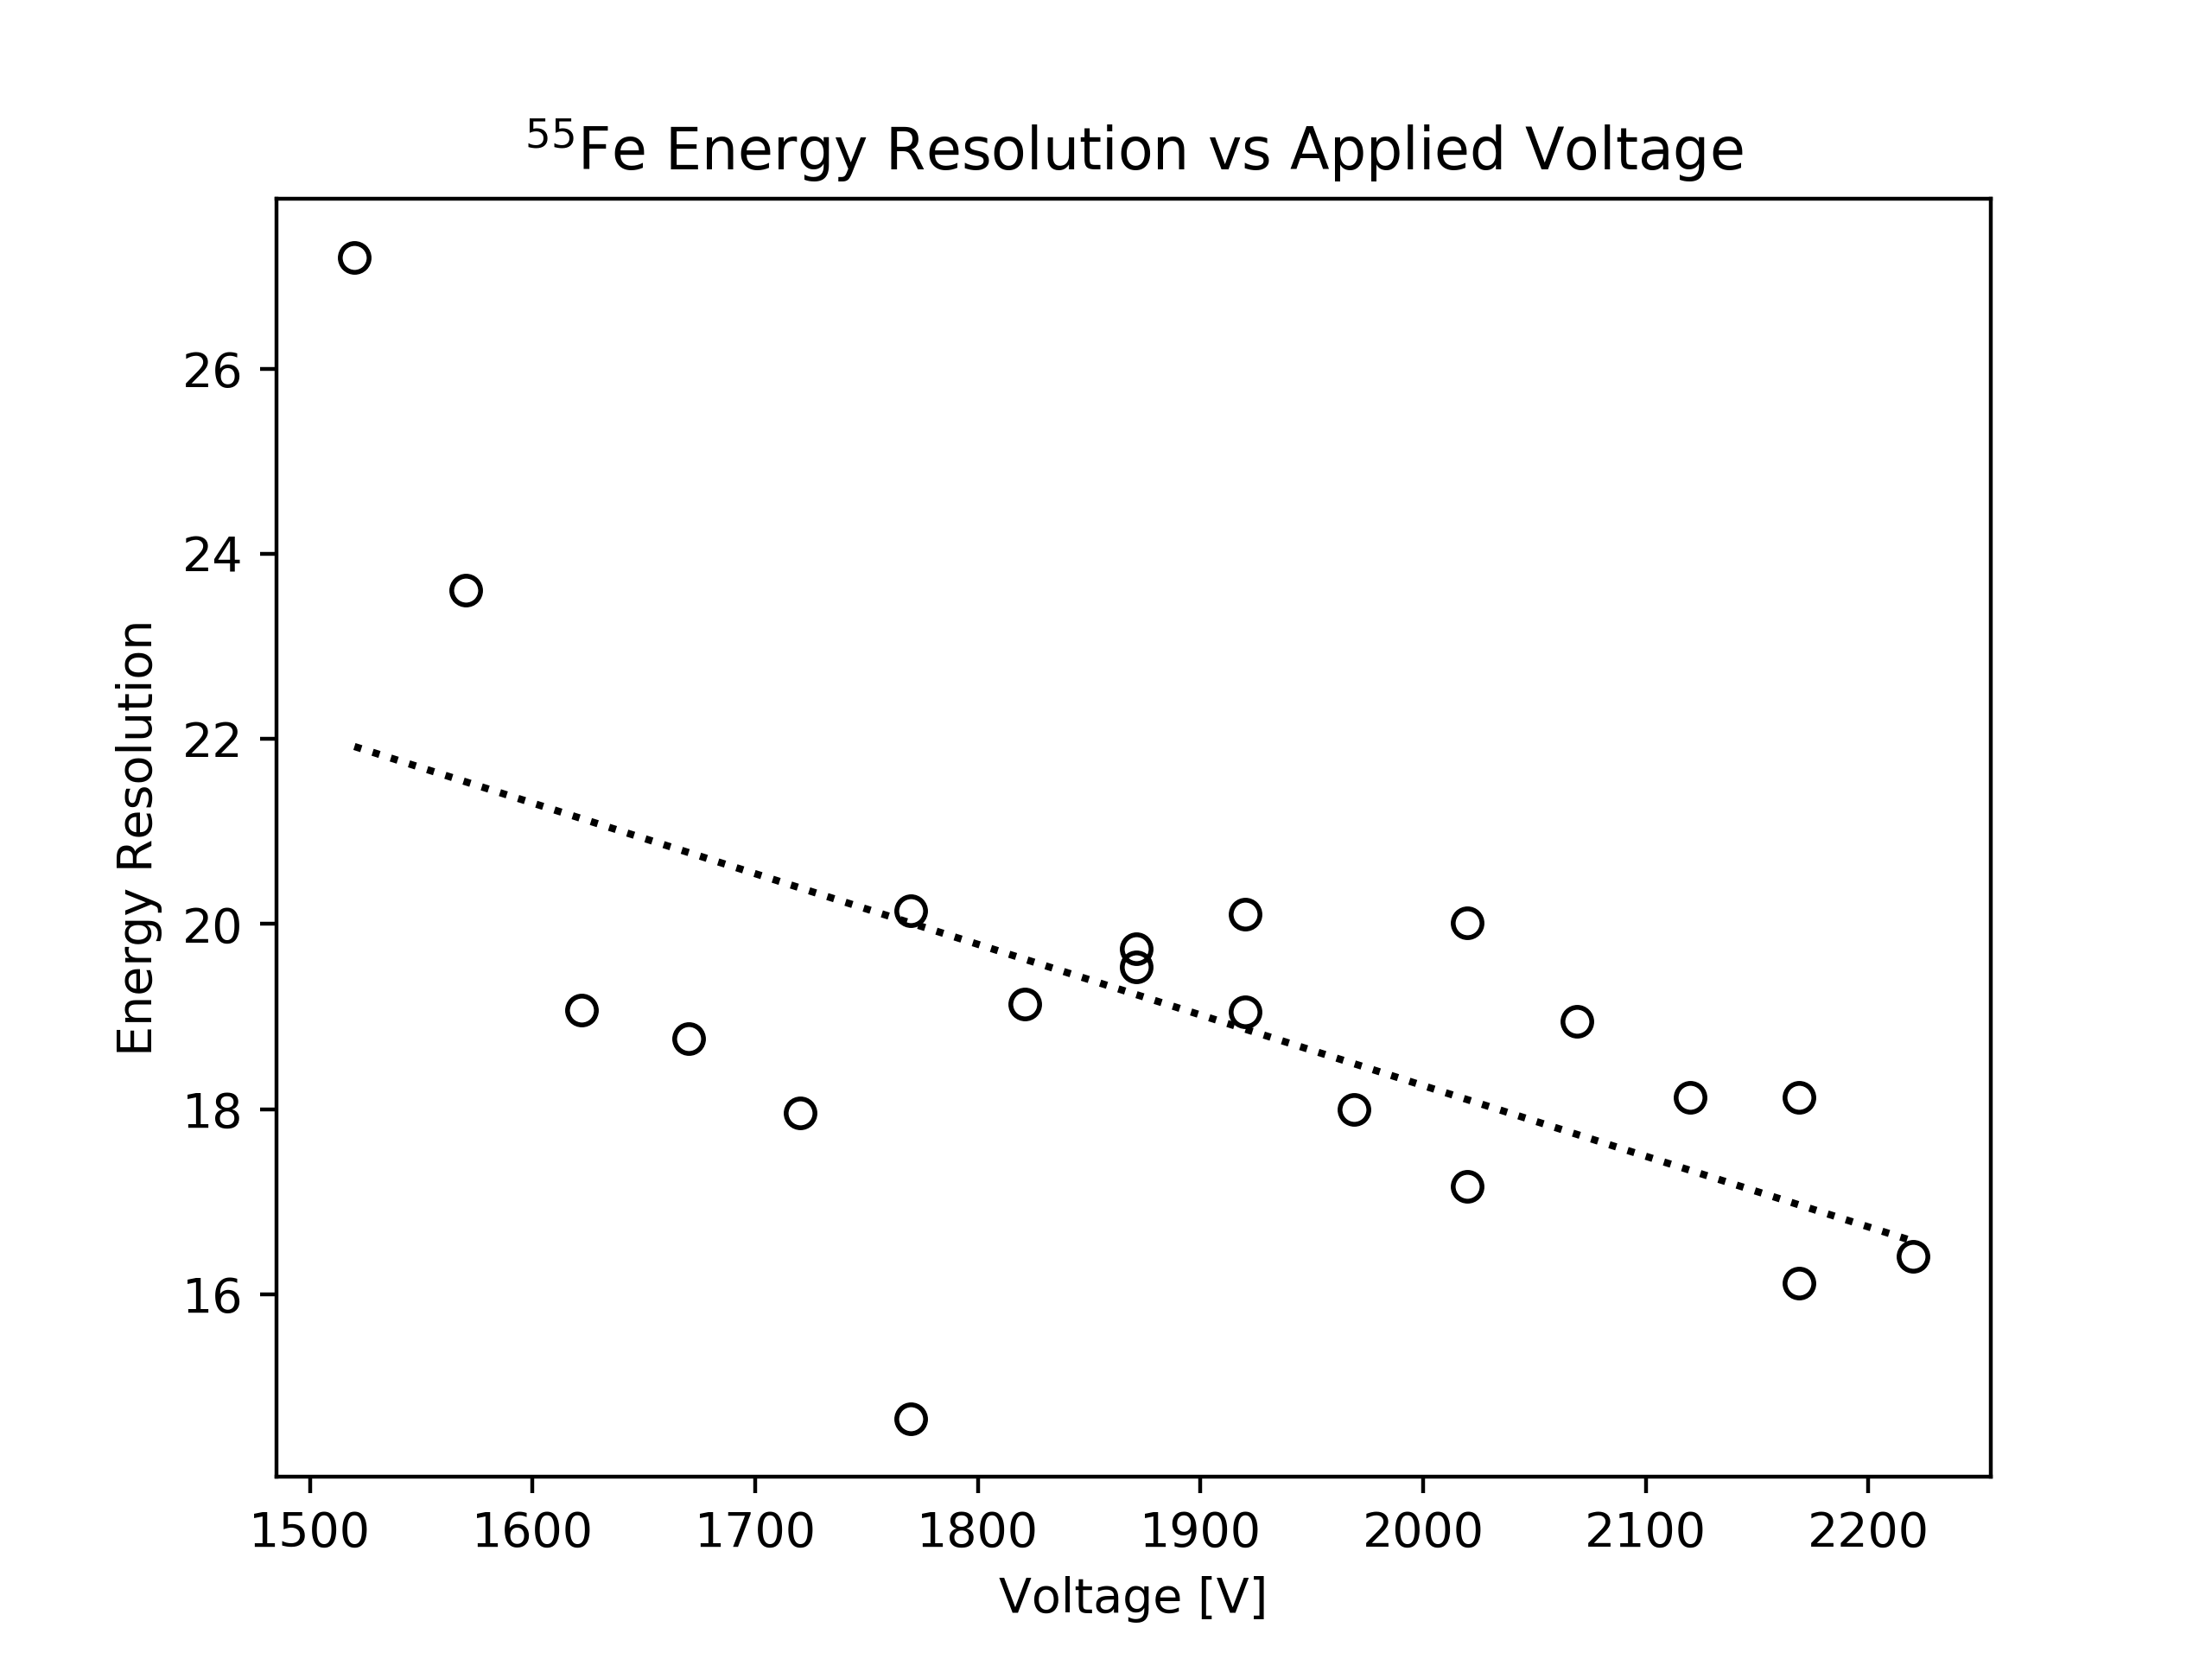
\includegraphics[width=12cm]{EResVsVFe.png}
  \caption{Graph of the energy resolution while measuring \textsuperscript{55}Fe, plotted against applied voltage.}
  \label{fig:EResVsVFe}
\end{figure}

\begin{figure}[H]
  \centering
  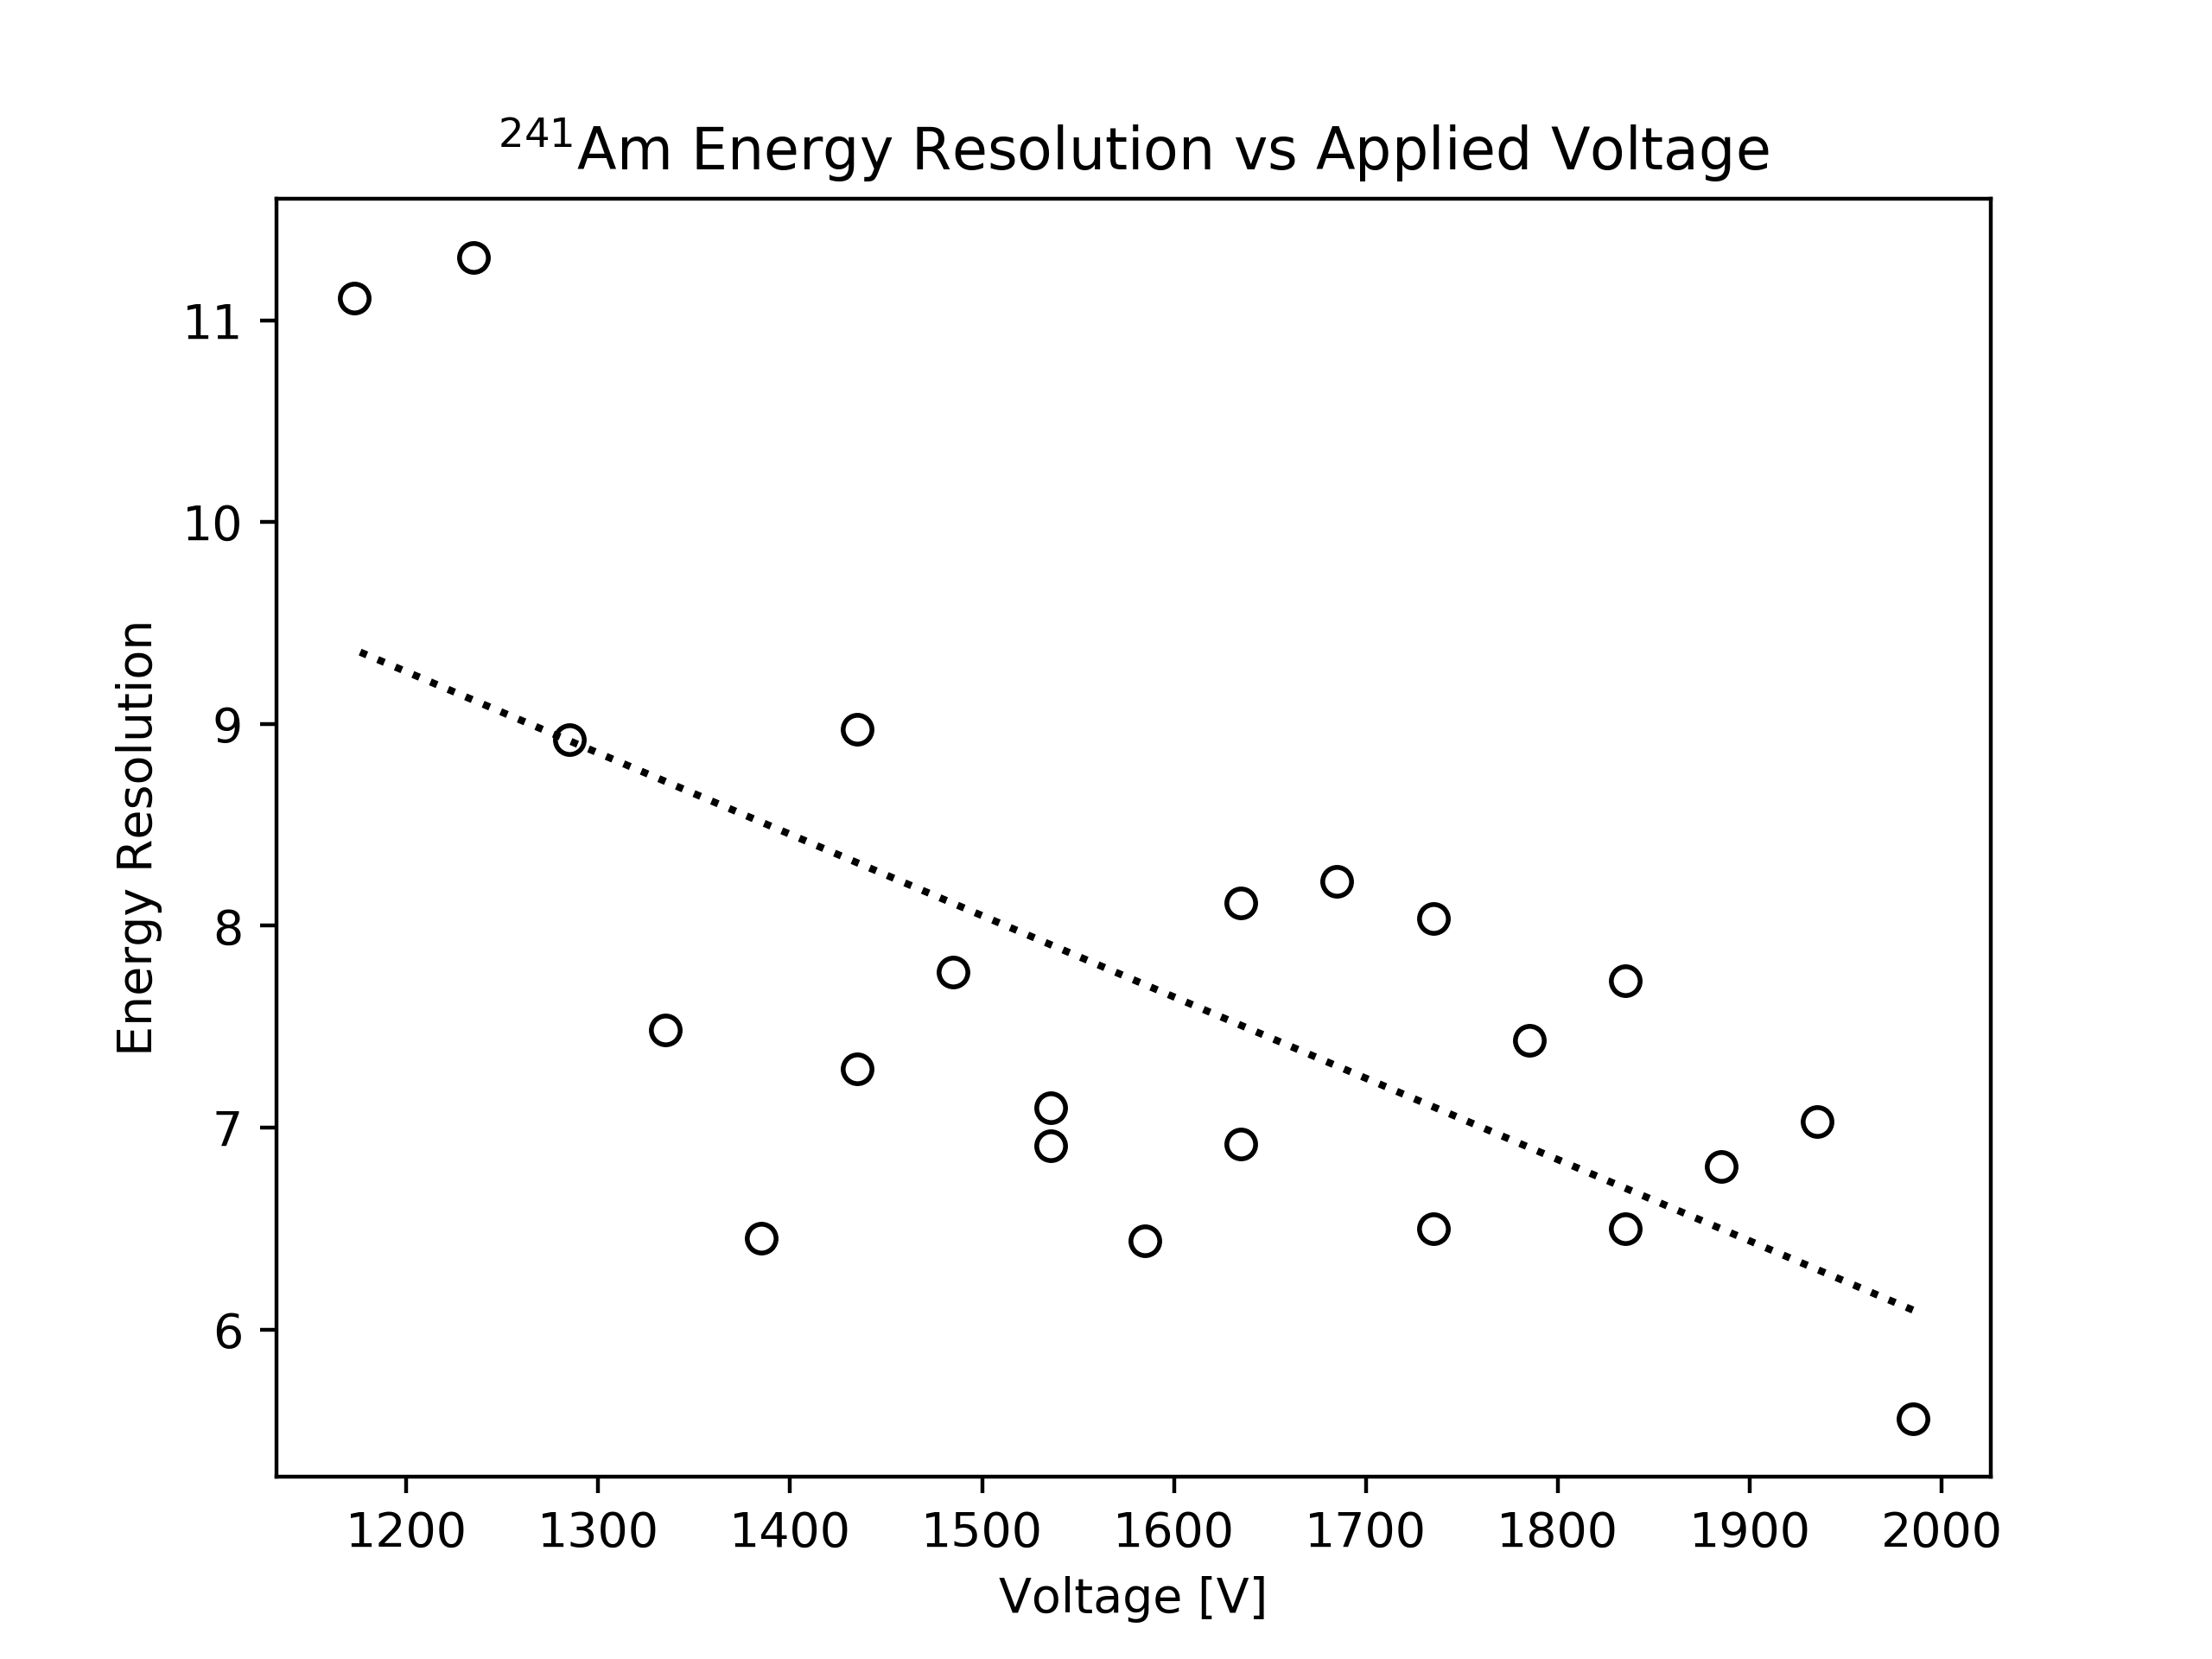
\includegraphics[width=12cm]{EResVsVAm.png}
  \caption{Graph of the energy resolution while measuring \textsuperscript{241}Am, plotted against applied voltage.}
  \label{fig:EResVsVAm}
\end{figure}

\subsection{Spectra}

\begin{figure}[H]
  \centering
  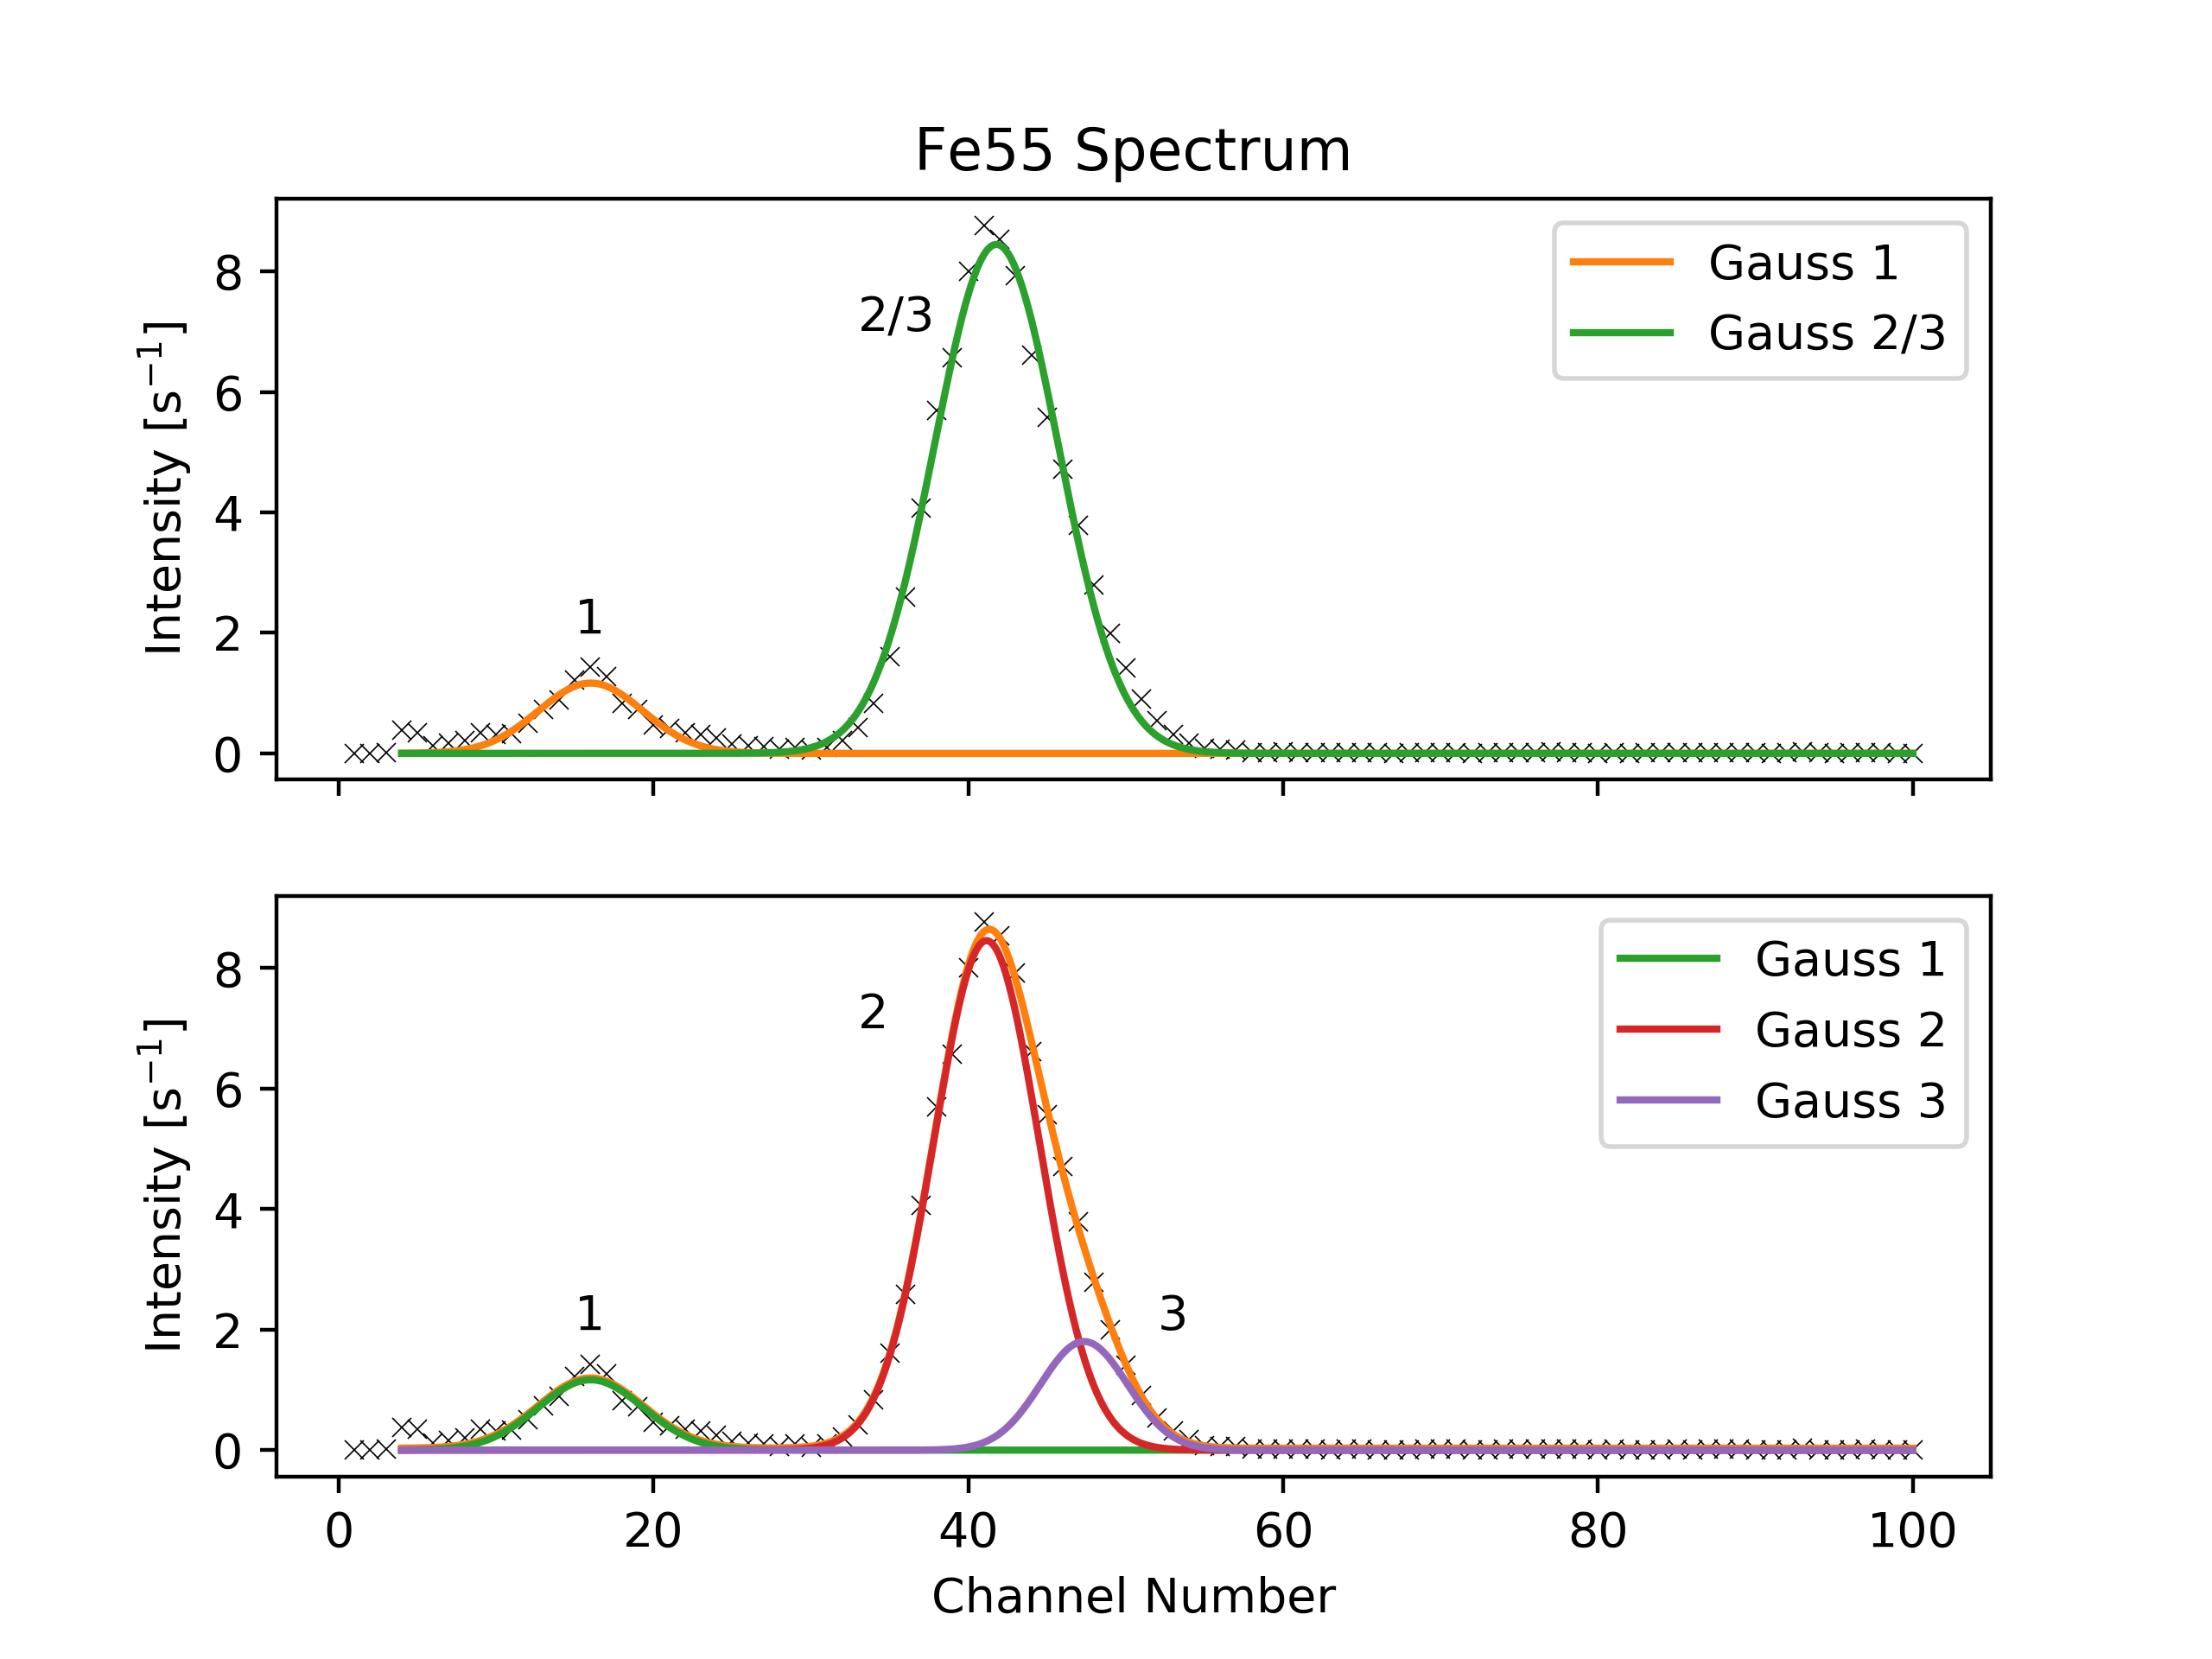
\includegraphics[width=9.93cm]{Fe55_spectrum.png}
  \caption{The spectrum of \textsuperscript{55}Fe from channels 0 to 100 because above 100 there were no spectral features. The top graph models the main photopeak as a single Gaussian curve, the bottom models it as two. The background in both cases was found to be almost negligible: (0.4$\pm$0.2) top; (0.3$\pm$0.1) bottom. The peak centres and FHWM are compiled in Table \ref{tbl:energyCalibration}.}
  \label{fig:Fe55spec}
\end{figure}

\begin{figure}[H]
  \centering
  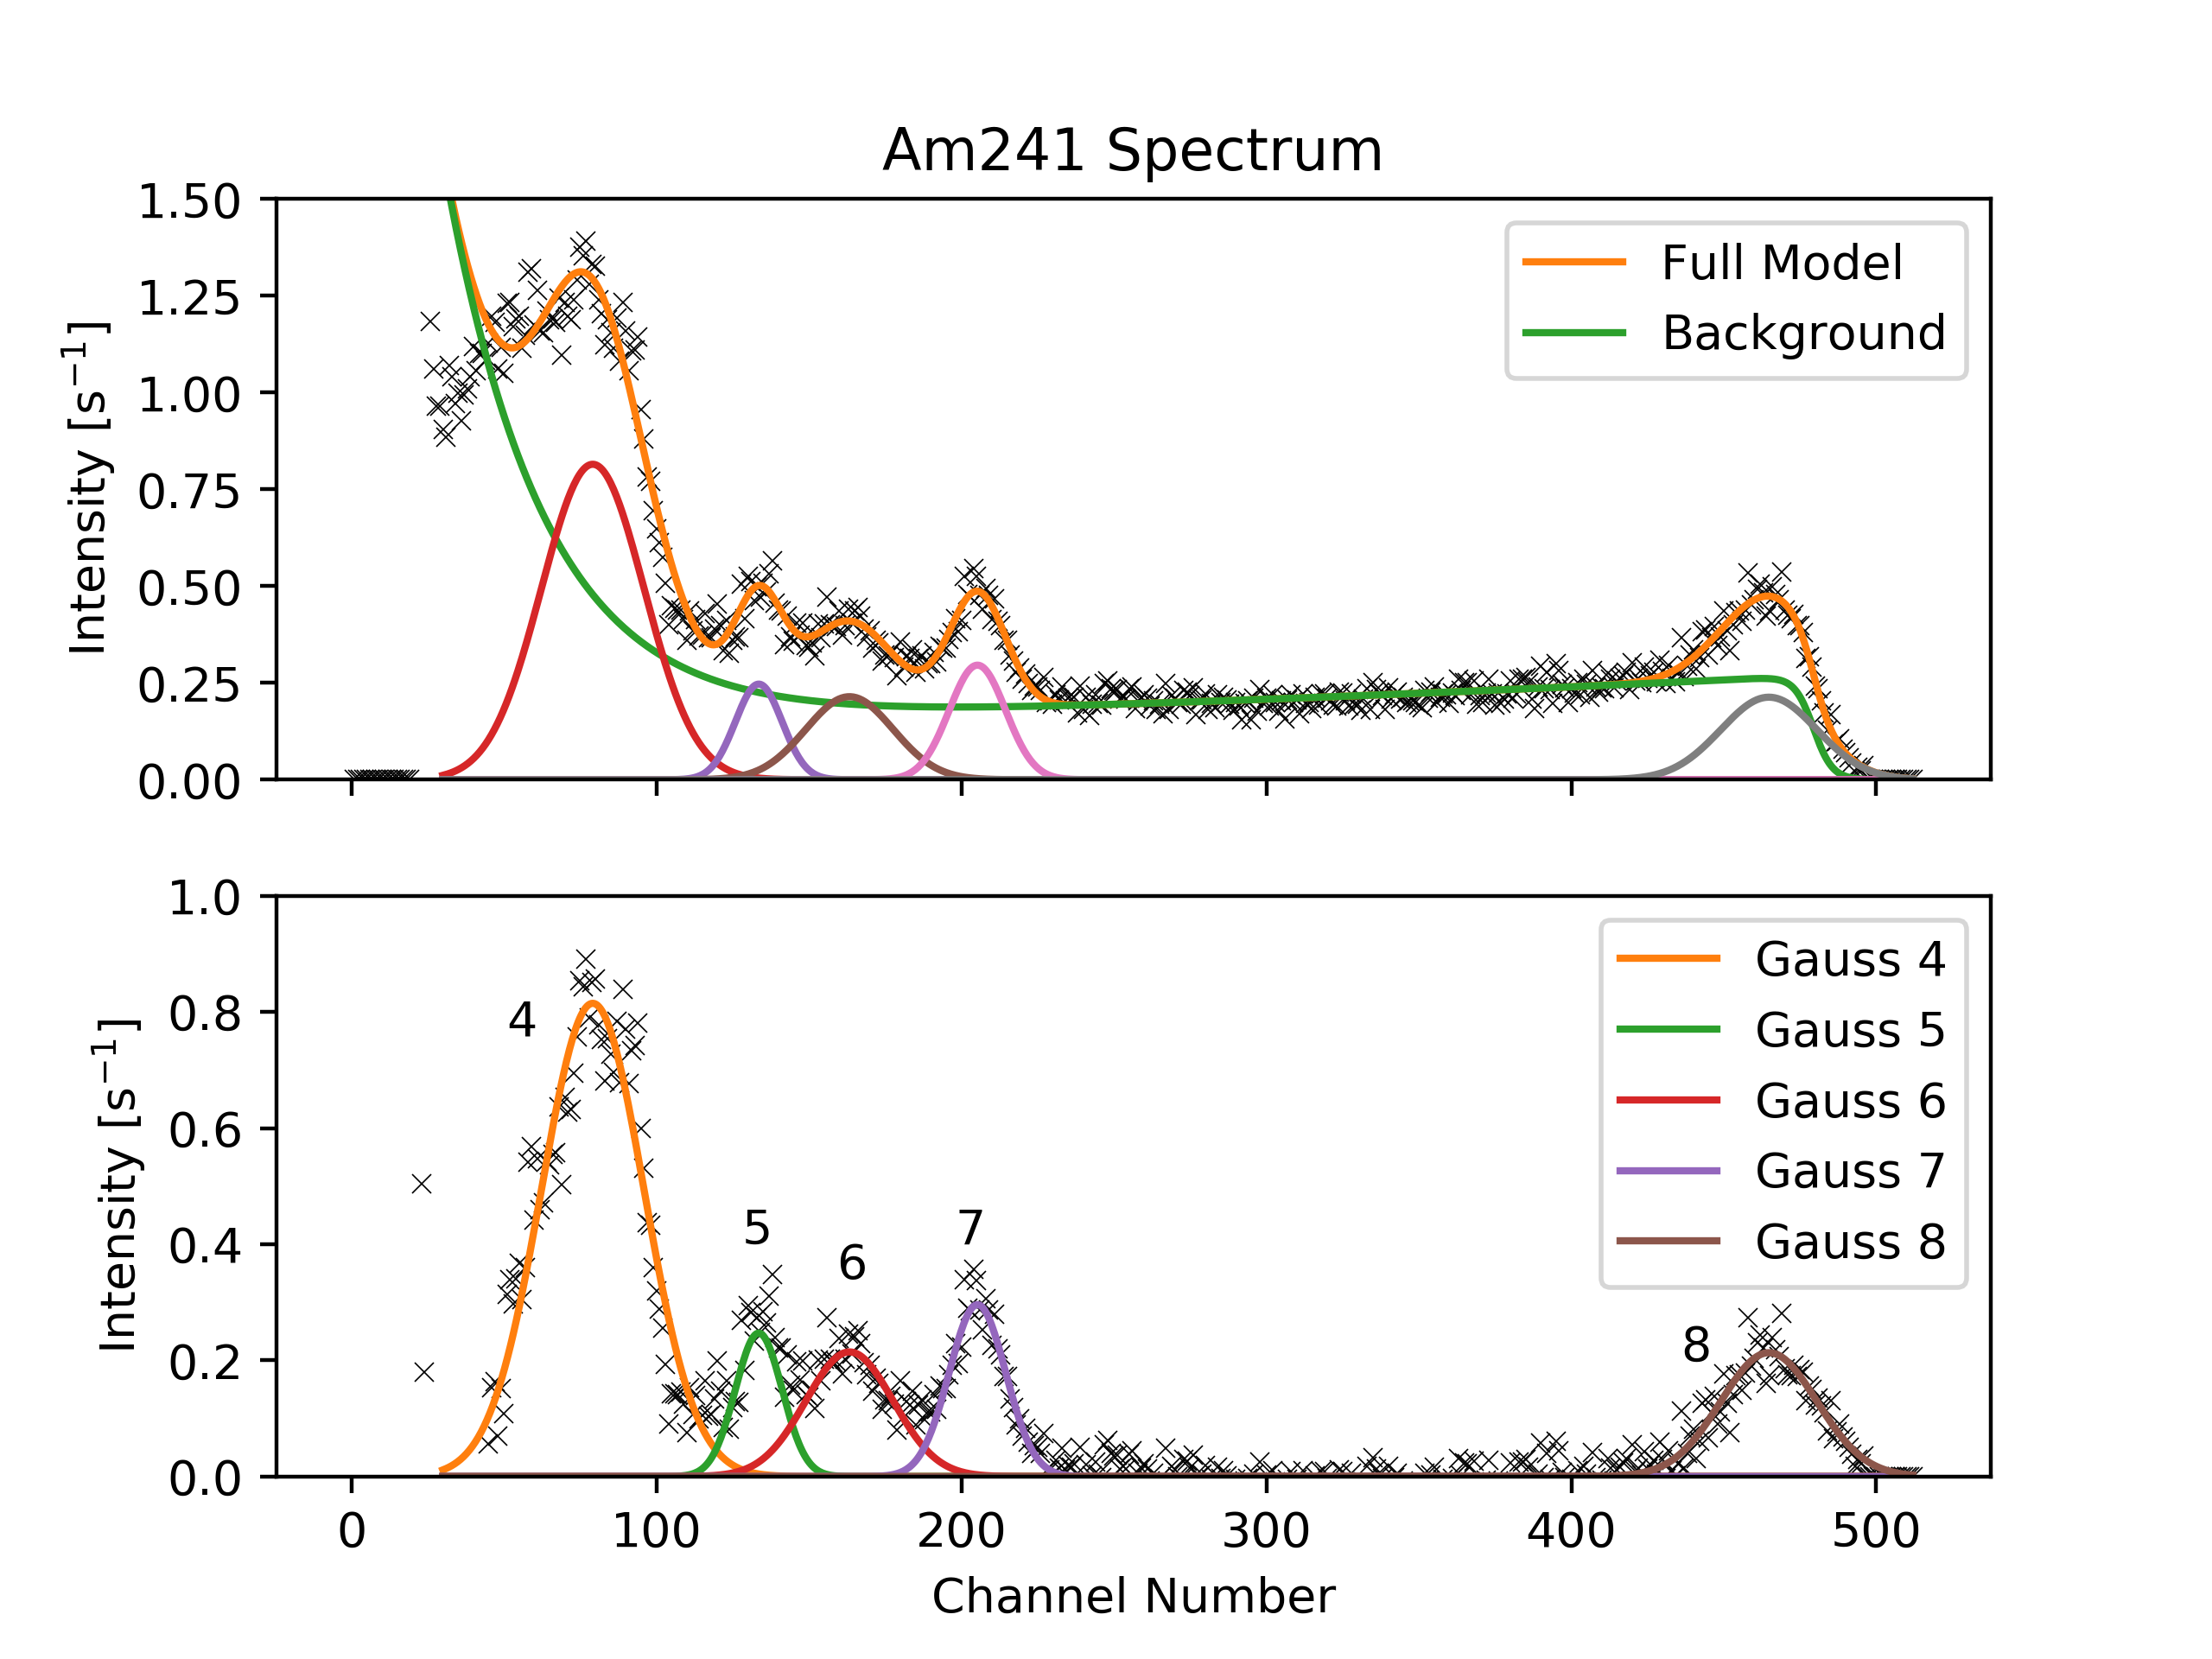
\includegraphics[width=9.93cm]{Am241_spectrum.png}
  \caption{The top graph shows the full spectrum of \textsuperscript{241}Am and the fitted model. The bottom graph shows the spectrum minus the background, leaving just the peaks. The parameters for the background were found to be: a$_{1}$ = (3.7$\pm$0.9), b$_{1}$ = (-0.030$\pm$0.007), a$_{2}$ = (0.13$\pm$0.01), b$_{2}$ = (0.0014$\pm$0.0003), c = (479$\pm$1), d = (3.1$\pm$0.8). The peak centres and FHWM are compiled in Table \ref{tbl:energyCalibration}.}
  \label{fig:Am241spec}
\end{figure}

\subsection{Energy Calibration}

\begin{table}[H]
    \begin{tabular}{llll}
    \hline \hline
    Peak & Channel  & Energy [keV] & FWHM [keV]  \\ \hline
    1    & 16.0$\pm$1    & 3.20 (Calib.)          & 0.97$\pm$0.02   \\
    2    & 41.2$\pm$0.1  & 5.89 (Calib.)        & 0.975$\pm$0.009 \\
    3    & 47.3$\pm$0.5  & 6.49 (Calib.)        & 0.80$\pm$0.03   \\
    4    & 79.1$\pm$0.4  & 10.78$\pm$0.05   & 4.9$\pm$0.2     \\
    5    & 133.6$\pm$0.9 & 17.5$\pm$0.1     & 2.2$\pm$0.1     \\
    6    & 163$\pm$1     & 21.15$\pm$0.04   & 4.2$\pm$0.2     \\
    7    & 205.3$\pm$0.6 & 26.37$\pm$0.09      & 2.69$\pm$0.08   \\
    8    & 465$\pm$1    & 59.54 (Calib.)       & 4.6$\pm$0.2     \\ \hline \hline
    \end{tabular}
    \label{tbl:energyCalibration}
    \caption{Peak centres as found by fitting models to the spectra with their respective energies. Those used for calibration are denoted with (Calib.) and have no uncertainty as they are book values.}
\end{table}

\begin{figure}[H]
  \centering
  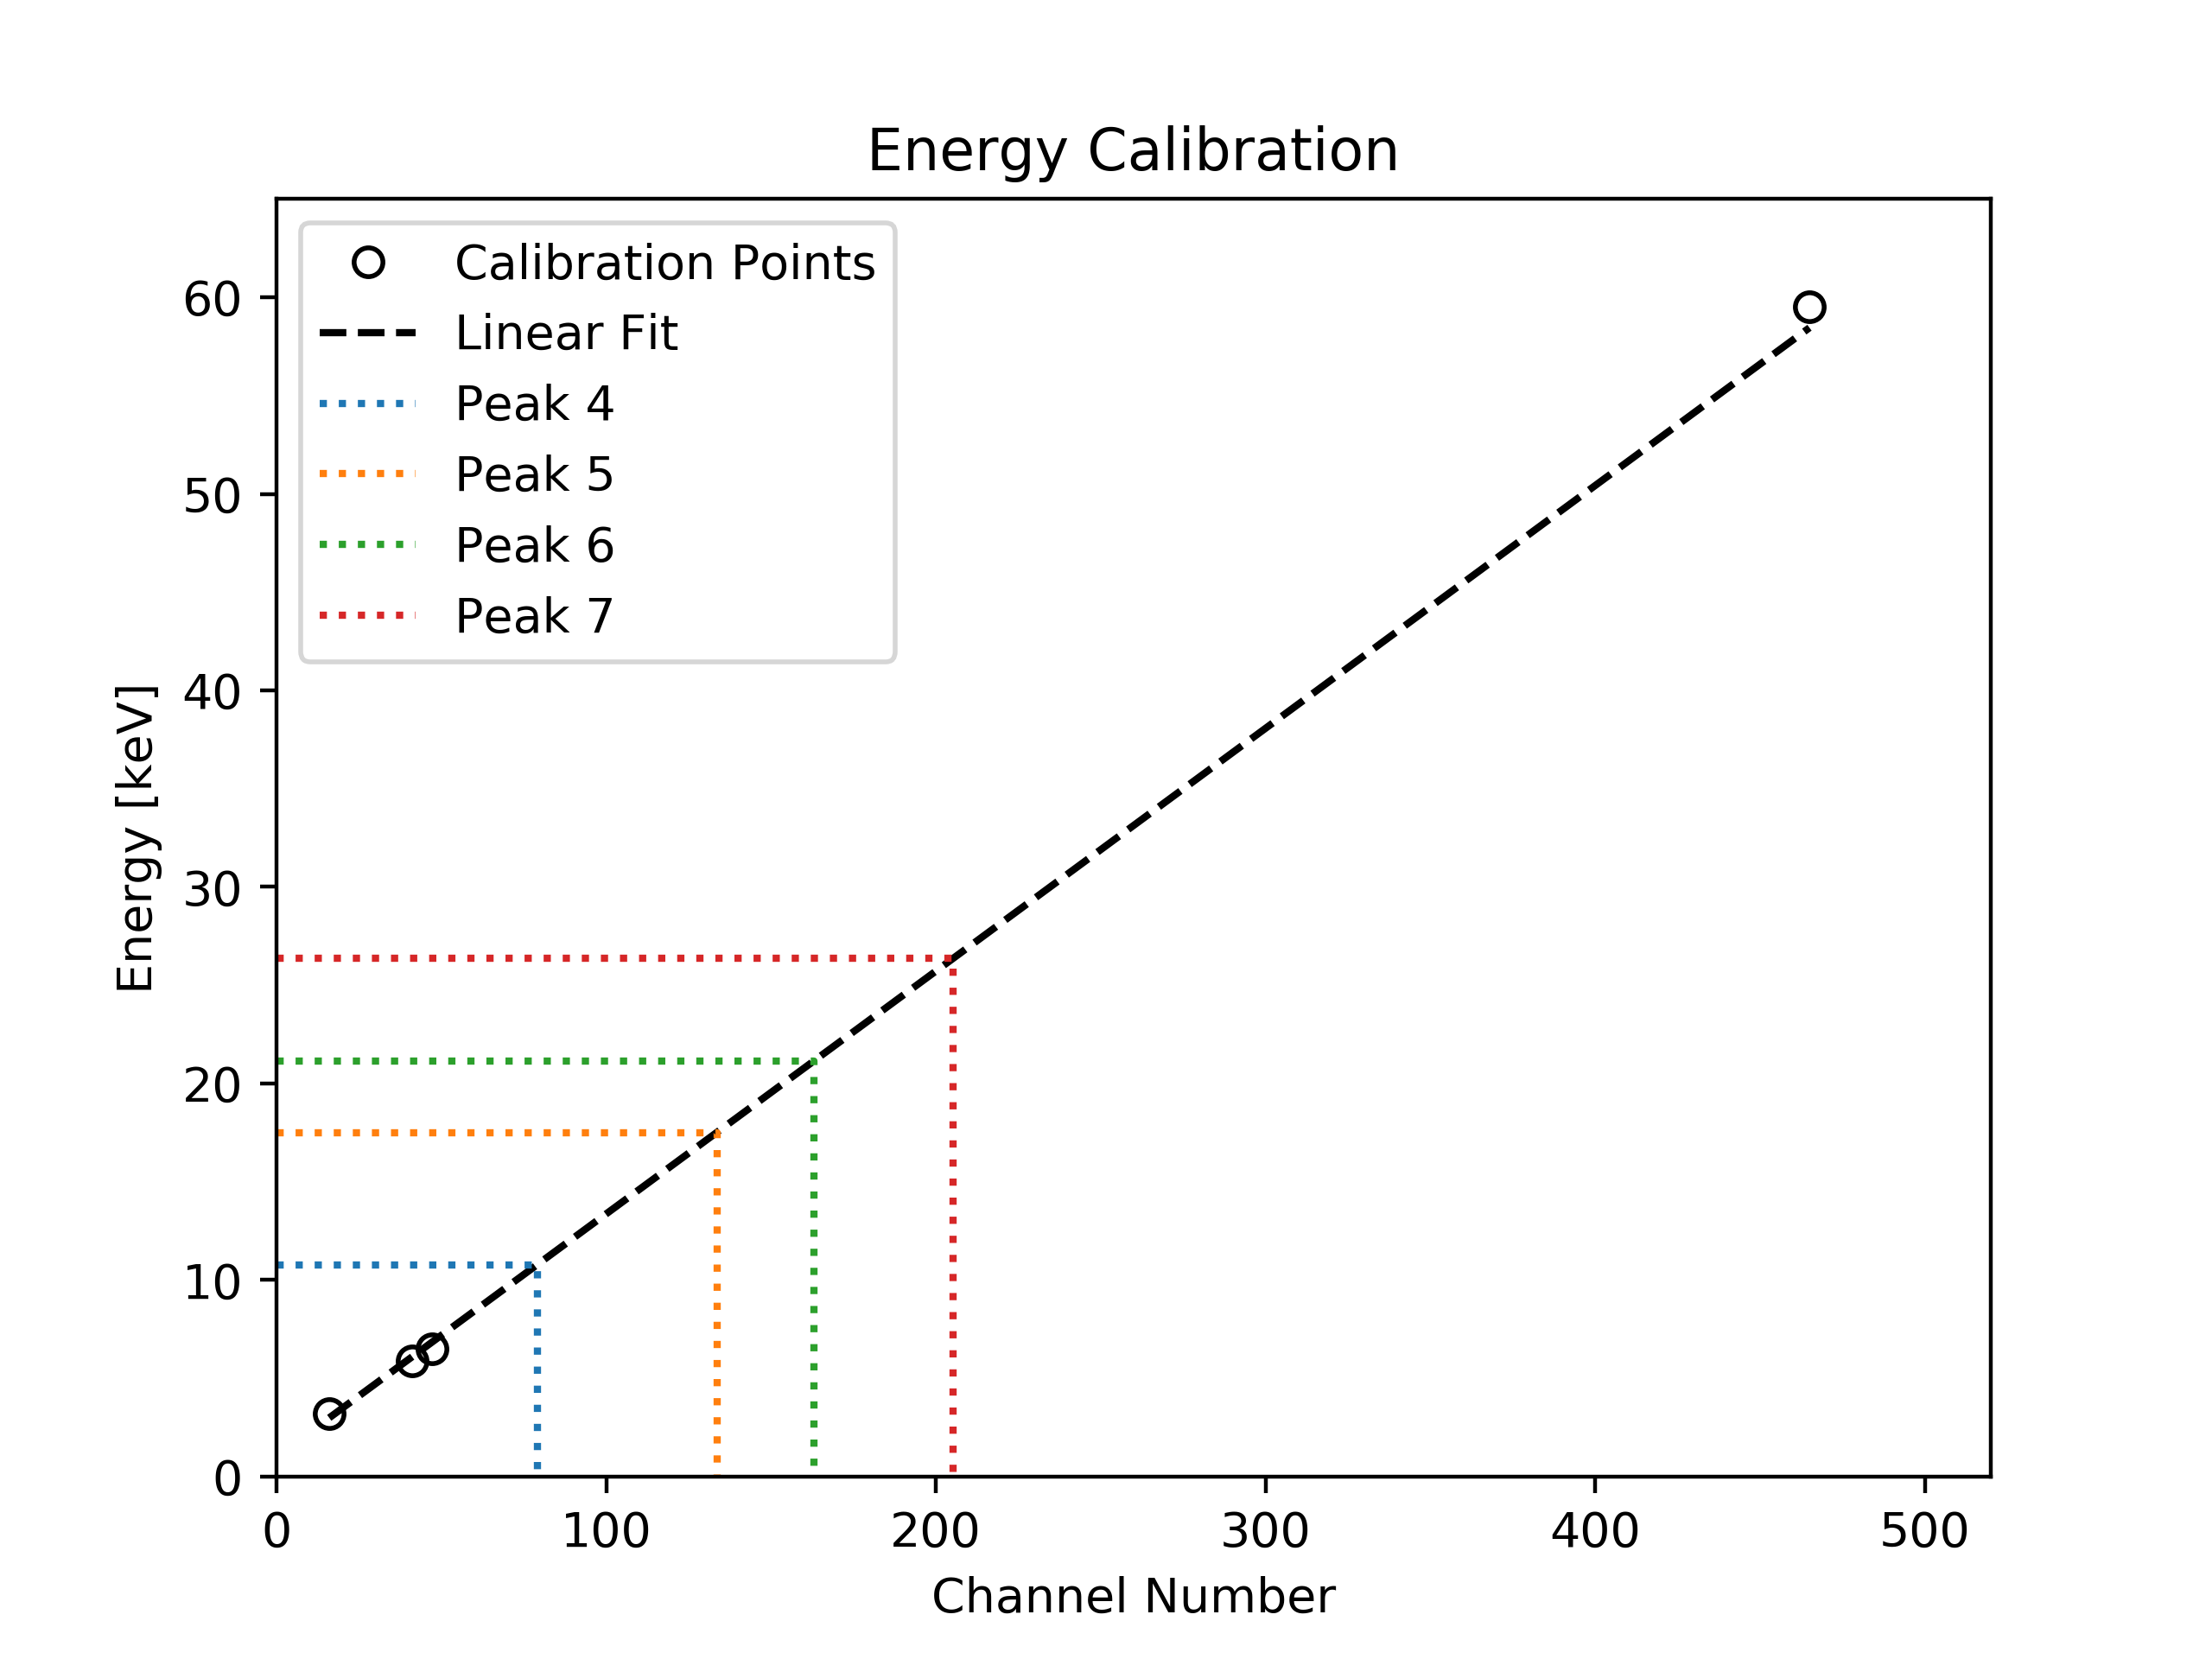
\includegraphics[width=\linewidth]{energyCalibration.png}
  \caption{Plot of channel centre against energy. The fitted linear model gave the conversion equation between particle energy and channel number to be: $E = (0.1235\pm0.0003)Ch + (1.01\pm0.01)$}
  \label{fig:energyCalibration}
\end{figure}

\section{Preamplifier}

\begin{figure}[H]
  \centering
  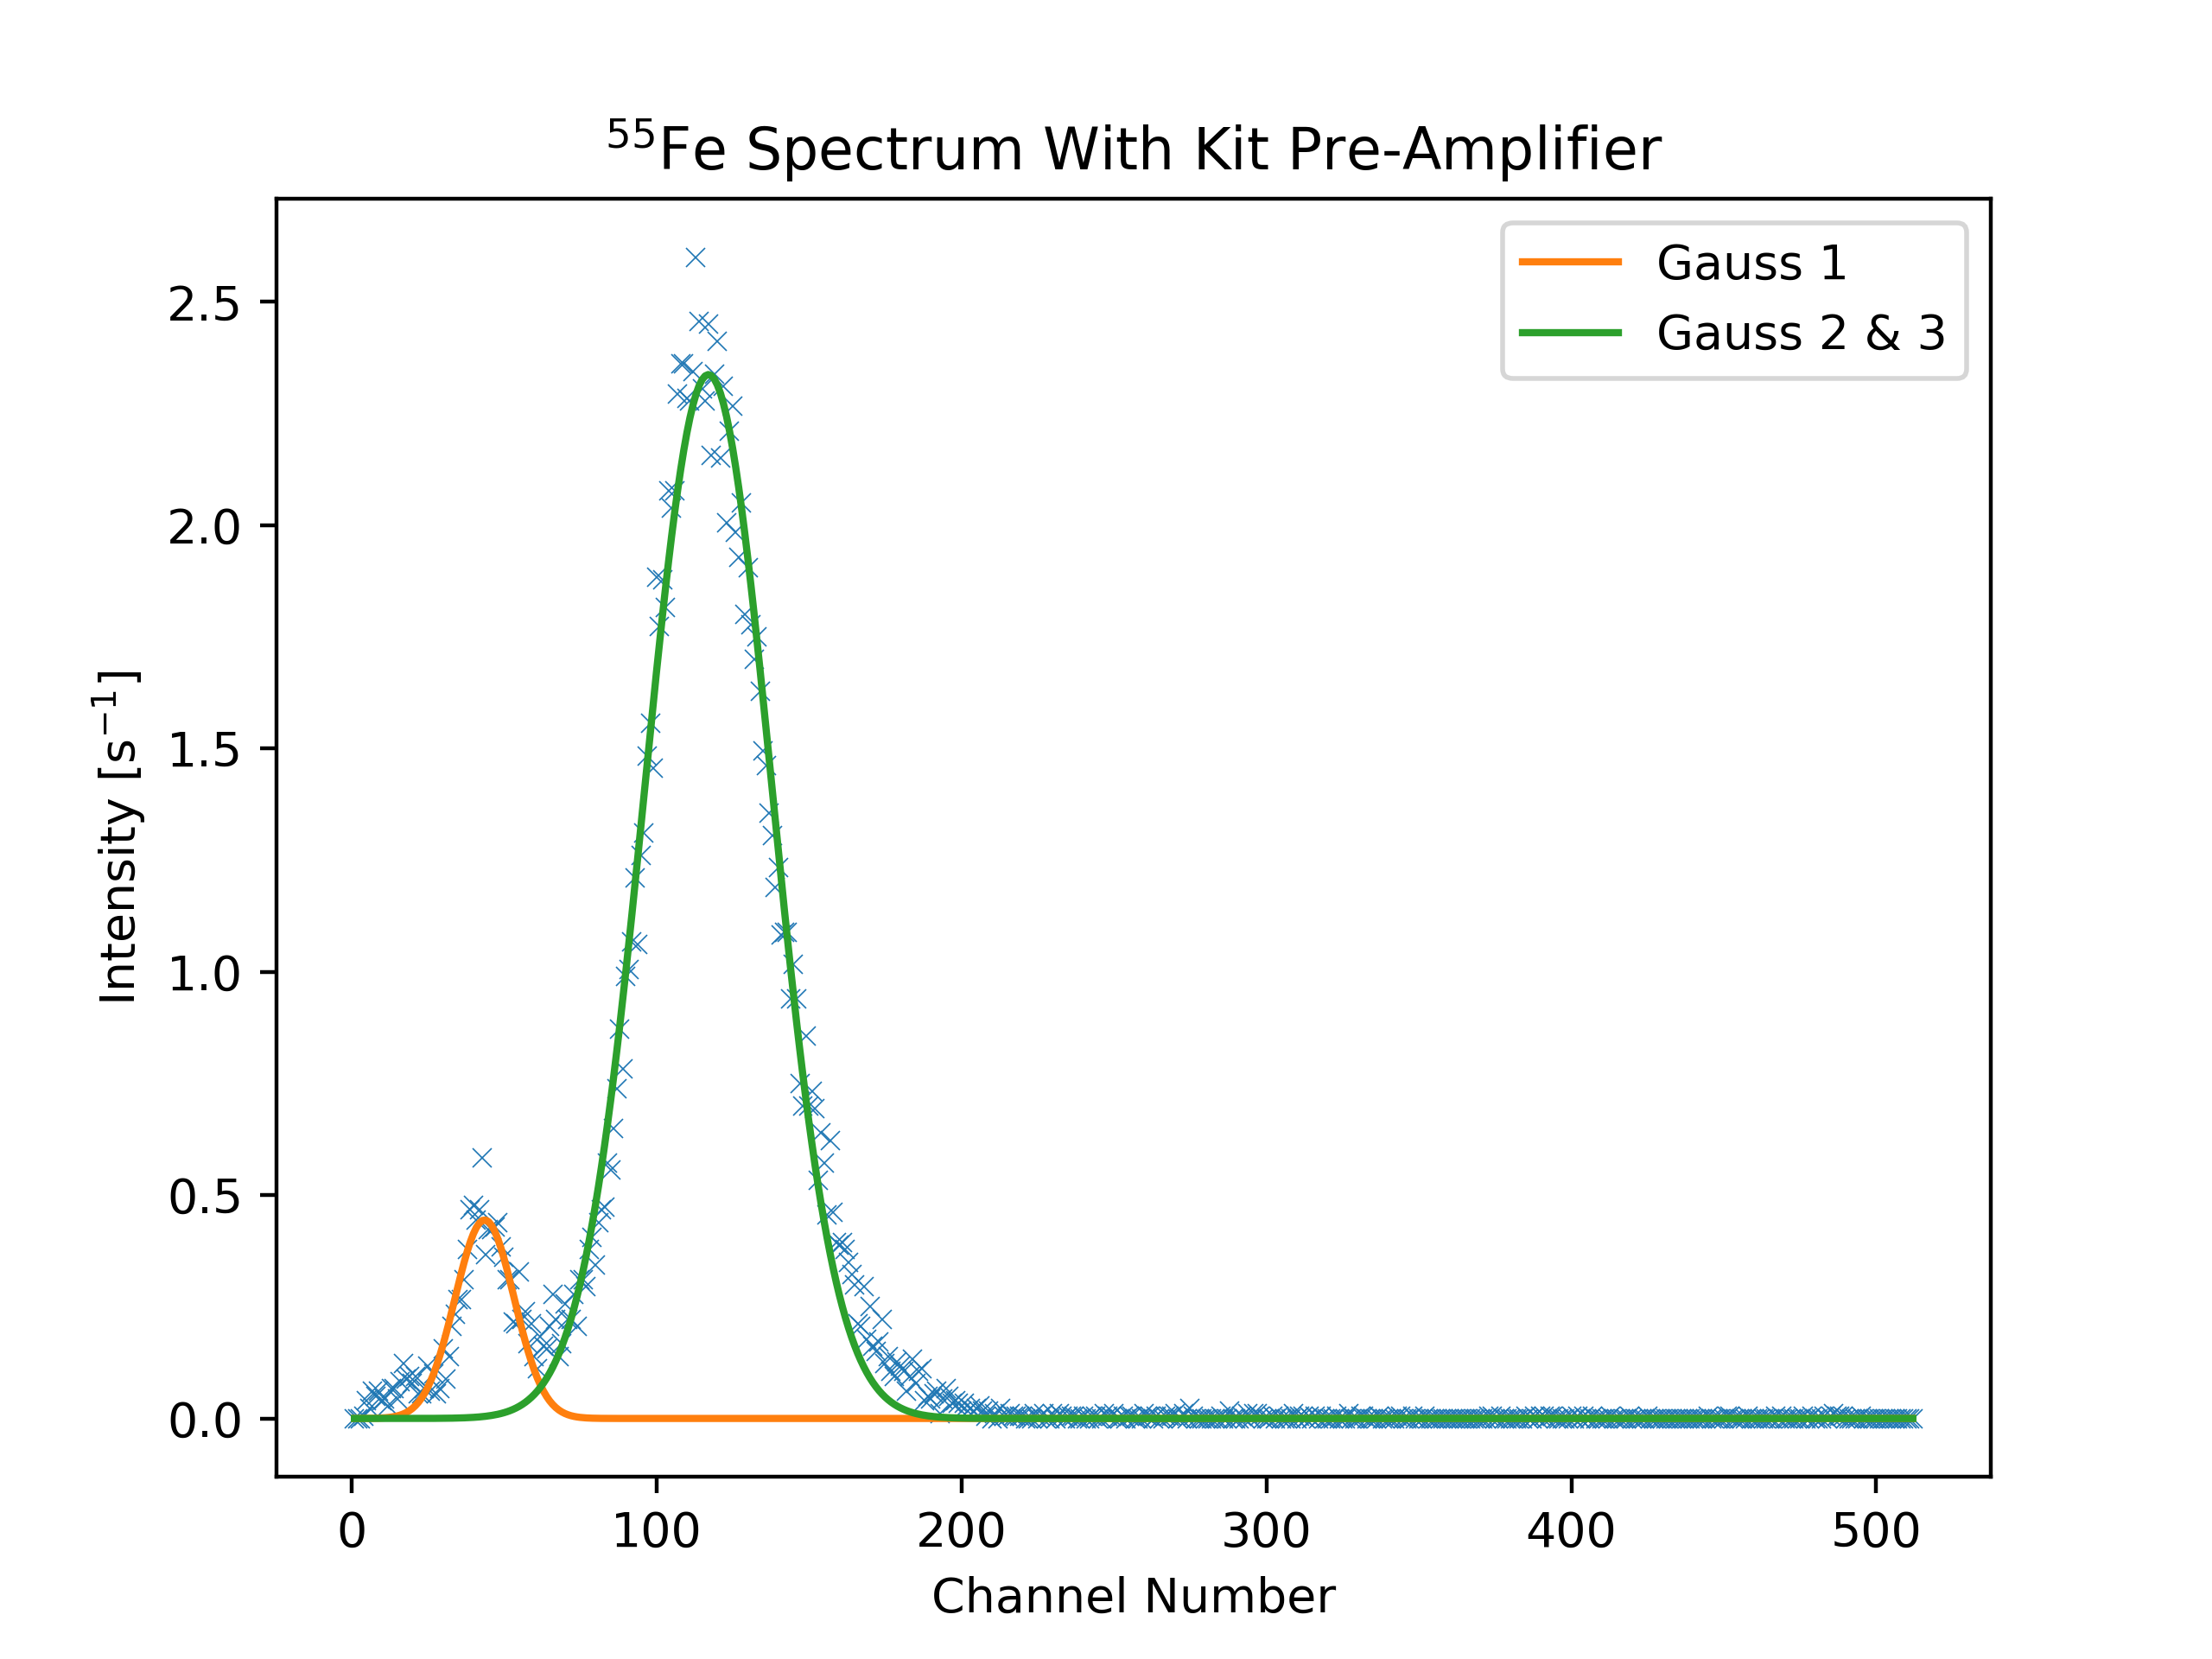
\includegraphics[width=\linewidth]{preamplifierSpectrum.png}
  \caption{Spectrum of \textsuperscript{55}Fe, measured using the kit preamplifier. The Gaussian curve fitted to the main photopeak was found to have a channel centre of (177.1$\pm$0.2) and a FWHM of (48.9$\pm$0.4). This means the peak has an energy resolution of (23.7$\pm$0.2)\%.}
  \label{fig:preampSpec}
\end{figure}
%%%%%%%%%%%%%%%%%%%%%%%%%%%%


%%%%%%%%%%%%%%%%%%%%%%%%%%%%
% DISCUSSION

\chapter{Discussion}

\section{Detector}

\subsection{Electron Calibration}
The linearity of the multichannel analyser's voltage response is attested by the agreement of the calibration data with a straight line fit (Figure \ref{fig:calibration}). The fitted line equation gives a conversion equation of:
\begin{equation}
    n_{e} = (2030\pm20)Ch
\end{equation}
Where n\textsubscript{e} is the number of collected electrons and Ch is the channel number. Two models were tested and the model with no constant was chosen due to its theoretical grounding whilst the fitted constant parameter was dominated by uncertainty in the other.

The dominating uncertainty in the plot is the uncertainty resulting from pulse amplitude. This is incorporated in the uncertainty of the calibration equation and will be carried forward when the equation is used in future calculations.

\subsection{Voltage Run}

Both voltage scans with \textsuperscript{55}Fe and \textsuperscript{241}Am, proved to be well described by an exponential model. At lower voltages the data points for both \textsuperscript{55}Fe and \textsuperscript{241}Am appear to stray from the trend line. This could be because at low voltages the detector moves out of the proportional region.

The datapoints with lower number of detected electrons have strikingly large errorbars. This is due to the fact that the graph's scale is logarithmic and these points have an error contribution which stays constant due to the spec amp, which is justified in Chapter \ref{sec:mthd:voltageRun}. Hence these errors are far more significant for smaller measured numbers of detected electrons.

\subsection{Multiplication Factor}

Plotting the multiplication factor for the \textsuperscript{55}Fe and \textsuperscript{241}Am sources on the same axis as that predicted by the Diethorn formula shows a very good agreement between the measured and theoretical results. All measured values fall within the range of uncertainty associated with the Diethorn formula, suggesting that the standard conditions for gas multiplication are met with this detector, such as a cylindrical magnetic field and a pure fill gas.

Again, the errorbars for lower multiplication factors are very large due to error propagation from the voltage run.

\subsection{Energy Resolution}

The energy resolution of the main photopeak for \textsuperscript{55}Fe and \textsuperscript{241}Am is (17.2$\pm$0.5)\% and (7.3$\pm$0.2)\% respectively. The energy resolution is much worse for \textsuperscript{55}Fe because the main photopeak is a superposition of two peaks which causes its FWHM to be much wider than if it where a single emission line like for \textsuperscript{241}Am.

Energy resolution follows a model of the form:
\begin{equation}
    \frac{E_{res}}{2.355} = \frac{\big( \sigma E \big)}{E} = \frac{a}{\sqrt{E}}+\frac{b}{E}+c
\end{equation}
Where $a$ is the detector dependent term and defines the intrinsic detector resolution, $b$ is the noise term and relates to the electronic noise, and $c$ is a constant term arising from the non-homogeneities such as geometry, calibration and energy leakage.
It can be seen from Figures \ref{fig:EResVsVFe} and \ref{fig:EResVsVAm} that energy resolution has a weak negative correlation with the applied voltage. Electronic noise and non-homogenities are unlikely to decrease with applied voltage, which implies intrinsic detector resolution improves with applied voltage.

\subsection{Spectra}

The spectrum for \textsuperscript{55}Fe was fitted extremely well by a three Gaussian model plus the background. However, the K$_{\alpha(1,2)}$ peak is approximately 5.7 times larger than the K$_{\beta(1,2)}$ peak, which is not supported by the relative intensities given by the decay tables which suggests a ratio of approximately 10 \cite{decay_modes}.

The spectrum for \textsuperscript{241}Am was far more complex with a relatively high background trailing the 59.54keV peak. This is due to both Compton scattering losses and electrons hitting the chamber walls before imparting all their energy, resulting in a reading with a lower energy than the original photon. This phenomenon would be reduced by building the detector with a greater volume however this may lead to quenching as discussed in Chapter \ref{sec:intr:fillGases}.

\subsection{Energy Calibration}

Fitting a linear model to the data in Figure \ref{fig:energyCalibration} gives a calibration equation of:
\begin{equation}
    E = (0.1235\pm0.0003)Ch + (1.01\pm0.01) \  [keV]
\end{equation}

Using this equation, the energies of peaks 4, 5, 6 and 7 were found (\ref{tbl:energyCalibration}), allowing their emission process to be identified.

Peak 5 was found to have an energy of (17.5$\pm$0.1)keV, this means it falls within the range of energies expected from the L$_{\beta}$ emission mechanism of (16.13-17.79)keV. Peak 6 was found to have an energy of (21.15$\pm$0.04)keV, this means it falls within the range of energies expected from the L$_{\gamma}$ emission mechanism of (20.12-22.20)keV. The FWHM of peaks 5 and 6 are (2.2$\pm$0.1)keV and (4.2$\pm$0.2) respectively which further supports attributing them to L$_{\beta}$ and L$_{\gamma}$. This is because the range of energies of the L$_{\beta}$ mechanism is approximately double that of L$_{\gamma}$ as is the case with the FWHM of peaks 5 and 6.

Peak 7 was found to have an energy of (26.37$\pm$0.09)keV. This means it can be attributed to the $\gamma_{2,1}$ emission mechanism which has a well defined energy of 26.34keV, which falls within the measured value's range of uncertainty.

Peak 4 was found to have an energy of (10.78$\pm$0.05)keV with a FWHM of (4.9$\pm$0.2). Upon close inspection of the spectrum it appears as though it may be a split peak. Fitting two Gaussian curves may have shifted this energy up to align with the $\gamma_{10,9}$ peak, or fall within the L$_{\alpha}$ range of energies, however there would still be one unknown peak left.

\section{Preamplifier}

The expected gain was 46.8 and it was measured on the oscilloscope as (45$\pm$2), thus falling within the acceptable range of uncertainty. This suggests that the device was working as it should, which was then proved when the spectrum of \textsuperscript{55}Fe was measured. The spectral features were clear, despite the worsened energy resolution of (23.7$\pm$0.2)\% compared to (17.2$\pm$0.5)\% of the ORTEC.
%%%%%%%%%%%%%%%%%%%%%%%%%%%%


%%%%%%%%%%%%%%%%%%%%%%%%%%%%
% CONCLUSION

\chapter{Conclusion}

This low cost proportional counter has been shown to be capable of detecting $\gamma$-ray radiation with energies from a few keV up to tens of keV. It is expected that sources with lower energy radiation will see a sharp drop in detector efficiency as they cannot penetrate the detector wall, though this could be resolved by installing a Mylar window. Higher energy photons will experience a gradual decrease in efficiency as Argon absorption falls away logarithmically \cite{nist}.

Its proportionality and an impressive agreement with the theoretical Diethorn formula is evidence that despite the simplicity and low cost of production, the detector is still good enough to follow the same principles of operation as far more expensive detectors. The detector is capable of measuring the relative intensities and energies of sources and can therefore be used to measure the energy spectrum of sources once it has been calibrated.

The implementation of a kit built preamplifier resulted in an increase of energy resolution of only 37.8\%. However, despite the relative cost and ease of assembly, this setup still measured a recognisable \textsuperscript{55}Fe spectrum which could have been modelled and further analysed if needed.
%%%%%%%%%%%%%%%%%%%%%%%%%%%%


%%%%%%%%%%%%%%%%%%%%%%%%%%%%
% BIBLIOGRAPHY
\clearpage
\phantomsection
\addcontentsline{toc}{chapter}{References}
\printbibliography
%%%%%%%%%%%%%%%%%%%%%%%%%%%%


%%%%%%%%%%%%%%%%%%%%%%%%%%%%
% START APPENDICES
\clearpage
\phantomsection
\appendix
\addcontentsline{toc}{chapter}{Appendix}
%%%%%%%%%%%%%%%%%%%%%%%%%%%%

\chapter{Electron Calibration}

\begin{figure}[h]
  \centering
  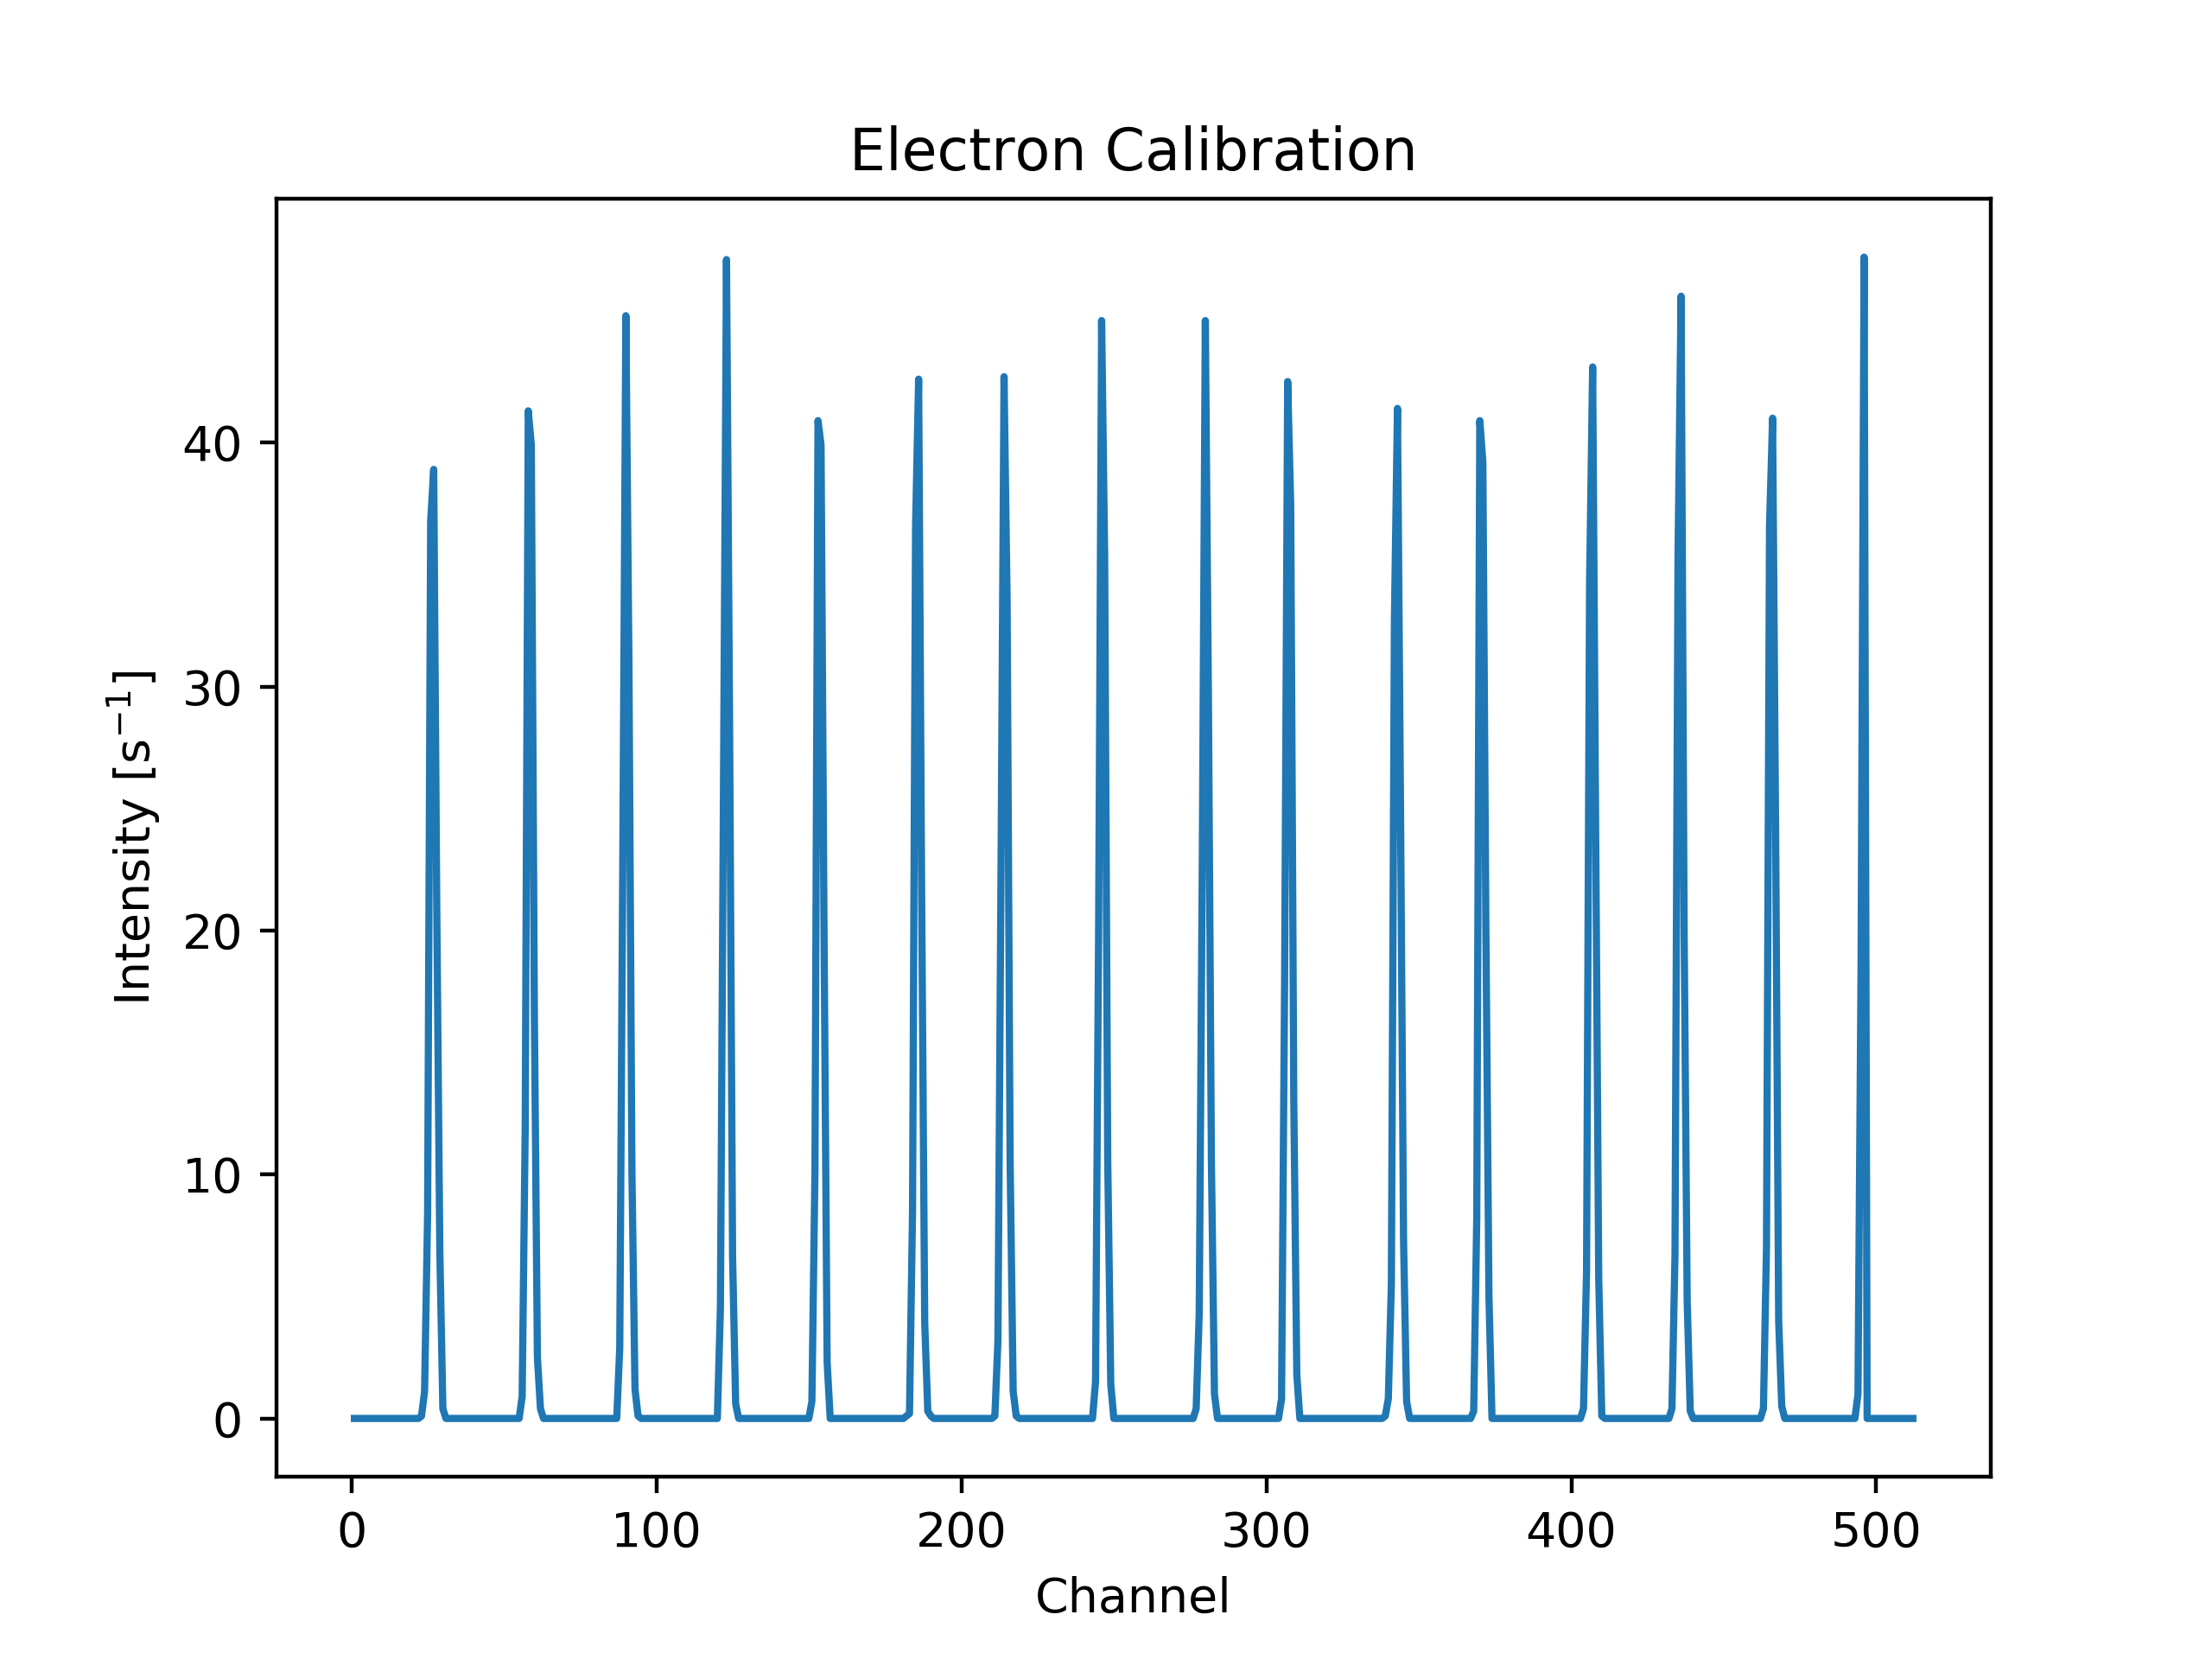
\includegraphics[width=\linewidth]{electronCalibrationData.png}
  \caption{The peaks measured in order to determine the relationship between detected charge and the channel it is registered in. These peaks were measured and compiled in \ref{tbl:electronCalibrationData}.}
  \label{fig:electronCalibrationData}
\end{figure}

\begin{table} \centering
  \begin{tabular}{lll}
    \hline
    \hline
    Pulse Amplitude [mV]     & Channel Centre       & FWHM \\ \hline
    9.7$\pm$0.2   & 26$\pm$3  & 2.52 \\
    19.6$\pm$0.2  & 58$\pm$3  & 2.32 \\
    29.7$\pm$0.2  & 89$\pm$3  & 2.33 \\
    40.4$\pm$0.3  & 122$\pm$3 & 2.25 \\
    50.2$\pm$0.3  & 152$\pm$3 & 2.25 \\
    60.0$\pm$0.3  & 185$\pm$8 & 2.29 \\
    69.4$\pm$0.4  & 213$\pm$3 & 2.37 \\
    79.8$\pm$0.5  & 245$\pm$3 & 2.25 \\
    91$\pm$1      & 279$\pm$3 & 2.43 \\
    99.4$\pm$0.5  & 306$\pm$3 & 2.28 \\
    110.0$\pm$0.9 & 342$\pm$3 & 2.46 \\
    119.0$\pm$0.5 & 370$\pm$3 & 2.32 \\
    130$\pm$1     & 406$\pm$2 & 2.30 \\
    140$\pm$1     & 435$\pm$3 & 2.26 \\
    150$\pm$1     & 465$\pm$3 & 2.32 \\ \hline \hline
  \end{tabular}
  \caption{Table containing the data used for the electron calibration graph, measured using the spectrum software.}
  \label{tbl:electronCalibrationData}
\end{table}

\chapter{Voltage Runs}

\begin{figure}[h]
  \centering
  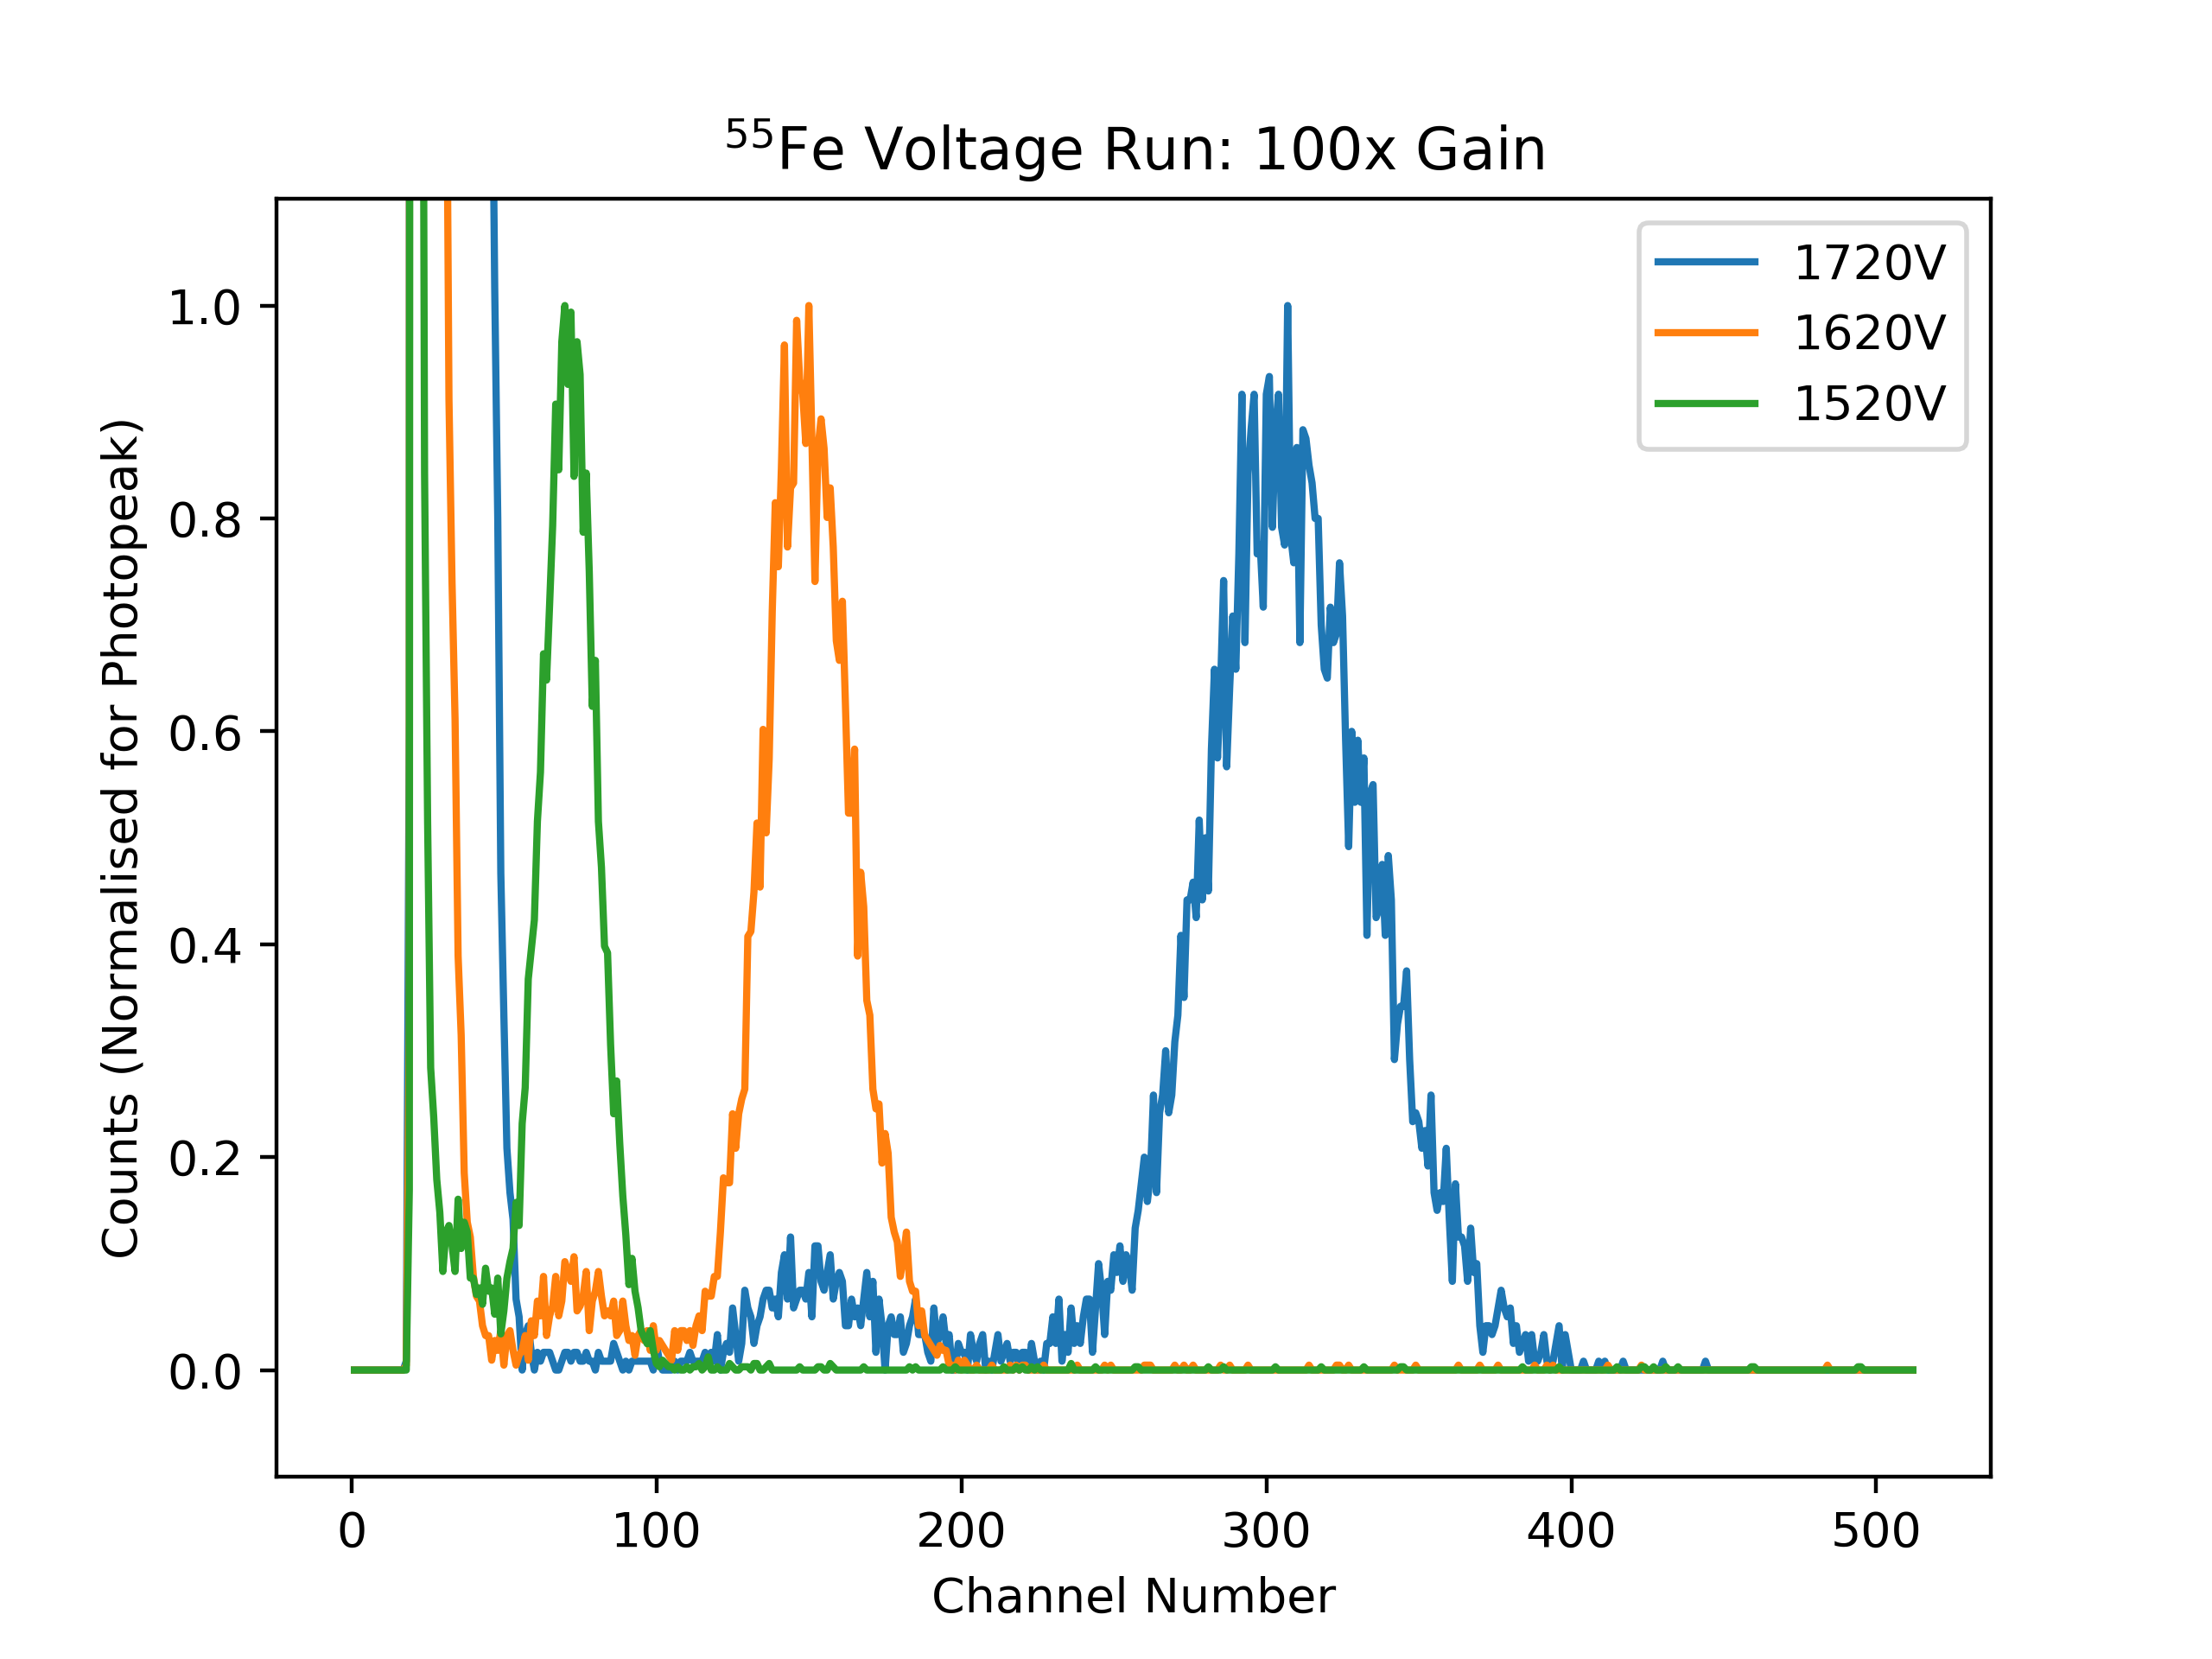
\includegraphics[width=\linewidth]{voltageRunData.png}
  \caption{Plot of example spectra, at a range of bias voltages with amplifier gain of 100. These spectra have been normalised.}
  \label{fig:voltageRunData}
\end{figure}

\begin{table}[]
\centering
\begin{tabular}{llll}
\hline \hline
Anode Bias {[}V{]} & Gain & Channel Centroid & FWHM \\ \hline
1520$\pm$4               & 100  & 70      $\pm$ 2           & 19   \\
1570$\pm$4               & 100  & 101              $\pm$ 1           & 24   \\
1622$\pm$4               & 100  & 147              $\pm$ 2           & 28   \\
1670$\pm$5               & 100  & 211              $\pm$ 1           & 40   \\
1720$\pm$5               & 100  & 306              $\pm$ 2           & 55   \\
1770$\pm$5               & 100  & 456.9            $\pm$ 0.8         & 67.0 \\
1770$\pm$5               & 40   & 179              $\pm$ 1           & 36   \\
1821$\pm$5               & 40   & 268              $\pm$ 1           & 51   \\
1871$\pm$5               & 40   & 391              $\pm$ 1           & 76   \\
1871$\pm$5               & 20   & 189              $\pm$ 1           & 37   \\
1920$\pm$5               & 20   & 281              $\pm$ 1           & 54   \\
1920$\pm$5               & 10   & 135              $\pm$ 1           & 27   \\
1969$\pm$5               & 10   & 200              $\pm$ 2           & 36   \\
2020$\pm$6               & 10   & 301              $\pm$ 2           & 52   \\
2020$\pm$6               & 4    & 122              $\pm$ 1           & 24   \\
2069$\pm$6               & 4    & 183              $\pm$ 2           & 35   \\
2120$\pm$6               & 4    & 283              $\pm$ 2           & 51   \\
2169$\pm$6               & 4    & 423              $\pm$ 2           & 68   \\
2169$\pm$6               & 2    & 206              $\pm$ 2           & 37   \\
2220$\pm$6               & 2    & 314              $\pm$ 2           & 52  \\ \hline \hline
\end{tabular}
\caption{Data measured when performing the voltage run with the \textsuperscript{55}Fe source.}
\label{tbl:feRun}
\end{table}

\begin{table}[]
\centering
\begin{tabular}{llll}
\hline \hline
Anode Bias {[}V{]} & Gain & Channel Centroid & FWHM \\ \hline
1173$\pm$3               & 100  & 77               $\pm$ 4           & 9    \\
1235$\pm$3               & 100  & 111              $\pm$ 3           & 13   \\
1285$\pm$4               & 100  & 153              $\pm$ 3           & 14   \\
1335$\pm$4               & 100  & 212              $\pm$ 3           & 16   \\
1385$\pm$4               & 100  & 293              $\pm$ 4           & 19   \\
1435$\pm$4               & 100  & 411              $\pm$ 3           & 30   \\
1435$\pm$4               & 40   & 161              $\pm$ 3           & 14   \\
1485$\pm$4               & 40   & 230              $\pm$ 3           & 18   \\
1536$\pm$4               & 40   & 328              $\pm$ 3           & 23   \\
1536$\pm$4               & 20   & 157              $\pm$ 3           & 11   \\
1585$\pm$4               & 20   & 226              $\pm$ 4           & 15   \\
1635$\pm$4               & 20   & 327              $\pm$ 3           & 23   \\
1635$\pm$4               & 10   & 156              $\pm$ 3           & 13   \\
1685$\pm$5               & 10   & 225              $\pm$ 3           & 18   \\
1735$\pm$5               & 10   & 331              $\pm$ 4           & 21   \\
1735$\pm$5               & 4    & 131              $\pm$ 3           & 11   \\
1785$\pm$5               & 4    & 192              $\pm$ 3           & 14   \\
1835$\pm$5               & 4    & 289              $\pm$ 4           & 19   \\
1835$\pm$5               & 2    & 137              $\pm$ 3           & 11   \\
1885$\pm$5               & 2    & 205              $\pm$ 4           & 14   \\
1935$\pm$5               & 2    & 304              $\pm$ 4           & 21   \\
1985$\pm$5               & 2    & 447              $\pm$ 5           & 25   \\ \hline \hline
\end{tabular}
\caption{Data measured when performing the voltage run with the \textsuperscript{241}Am source.}
\label{tbl:amRun}
\end{table}

%%%%%%%%%%%%%%%%%%%%%%%%%%%%


%%%%%%%%%%%%%%%%%%%%%%%%%%%%
% END DOCUMENT
\end{document}
%%%%%%%%%%%%%%%%%%%%%%%%%%%%